%~~~~~~~~~~~~~~~~ PREAMBULO ~~~~~~~~~~~~~~~~%
\documentclass[12pt,a4paper]{article}
\usepackage[english]{babel}
%\usepackage[T1]{fontenc}
\usepackage[utf8]{inputenc}
\usepackage{amsmath}
\usepackage{amssymb,amsthm}
\usepackage[usenames,dvipsnames]{color}
\usepackage{graphicx}
\usepackage{accents}
%\usepackage{wrapfig}
\usepackage{array}
\usepackage{color}
\usepackage{tcolorbox}
\usepackage{caption}
%\usepackage{subcaption}
\usepackage{fancybox}
\usepackage{fancyhdr}
\usepackage{extramarks}
%\usepackage{helvet}
\usepackage{colortbl}
\usepackage{subfig}
\usepackage{url}
\usepackage{hyperref}
\hypersetup{colorlinks=false,linkcolor=black}
\usepackage{mathrsfs}
\usepackage{latexsym}
%\usepackage{pstricks}
\usepackage{float}
\usepackage{graphics,psfrag}
%\usepackage{dsfont}
\usepackage{slashed}
%\usepackage[section]{placeins}
\usepackage{anysize}
\marginsize{2.5cm}{2.0cm}{2.0cm}{2.5cm}
\usepackage{verbatim}
\usepackage{sectsty}
\usepackage{appendix}
\usepackage{pgfplots}
\pgfplotsset{compat=newest}
\allsectionsfont{\sffamily}

\usepackage{tikz} 
\usetikzlibrary{chains,shapes,fit,calc}
\usetikzlibrary{positioning,arrows}

\usetikzlibrary{patterns,decorations.pathreplacing}
\usetikzlibrary{decorations.pathmorphing}
\usetikzlibrary{decorations.markings}
\usetikzlibrary{arrows,shapes}
\usetikzlibrary{shapes.misc}
\tikzset{
	gluon/.style={decorate, draw=black,
		decoration={coil,amplitude=4pt, segment length=4pt,aspect=0.7}} 
}
\tikzset{
	photon/.style={decorate, decoration={snake}},
}
%~~~~~~~~~~~~~~~~~~~~~~~~~~~~~~~~~~~~~~~~~~~%

%~~~~~~~~~~~~~~~ COMANDOS PROPIOS ~~~~~~~~~~~~~~%
\newcommand{\ket}[1]{|#1\rangle}
\newcommand{\bra}[1]{\langle#1|}
\newcommand{\braket}[2]{\langle#1|#2\rangle}
\newcommand{\crea}[2]{#1^{\dagger}_{#2}}
\newcommand{\des}[2]{#1_{#2}}
\newcommand{\grad}[1]{\vec{\nabla}#1}
\newcommand{\diver}[1]{\vec{\nabla}\vec{#1}}
\newcommand{\rotac}[1]{\vec{\nabla}\times#1}

\def\lag{\mathcal{L}}
\def\sw{\sin\theta_W}
\def\cw{\cos\theta_W}

\def\sW{s_W}
\def\cW{c_W}
\def\sWh{s_{\hat{W}}}
\def\cWh{c_{\hat{W}}}

\def\mz{{M_Z}}
\def\mw{{M_W}}

\def\hZ{{\hat{Z}}}
\def\hW{{\hat{W}}}
\def\hX{{\hat{X}}}

\def\Zp{Z^{'}}

\def\gZpuV{g_{\Zp}^{u,V}}
\def\gZpdV{g_{\Zp}^{d,V}}
\def\gZpuA{g_{\Zp}^{u,A}}
\def\gZpdA{g_{\Zp}^{d,A}}

\def\mathZ{\mathcal{Z}}
\def\mathA{\mathcal{A}}
\def\M{\mathcal{M}}
\def\b#1{\bar{#1}}

\def\Tr{{\rm Tr}}

%%%text under or over the sign
\newcommand{\equaltext}[1]{\ensuremath{\stackrel{#1}{=}}}
\newcommand{\approxtext}[1]{\ensuremath{\stackrel{#1}{\approx}}}
\newcommand{\arrowtext}[1]{\ensuremath{\stackrel{#1}{\longrightarrow}}}

%%%double hat using accents package
\newlength{\dhatheight}
\newcommand{\doublehat}[1]{%
	\settoheight{\dhatheight}{\ensuremath{\hat{#1}}}%
	\addtolength{\dhatheight}{-0.35ex}%
	\hat{\vphantom{\rule{1pt}{\dhatheight}}%
		\smash{\hat{#1}}}}

\def\p{\slashed{p}}
\definecolor{myblue}{cmyk}{0.65, 0.37, 0.0, 0.19}
\def\Mnote#1{{\color{myblue}[VM: #1]}} %Martin
\def\Cnote#1{{\color{blue}[DV: #1]}} %Cerdeno
\def\Vnote#1{{\color{green}[VR: #1]}} %Romeri
\def\met{\slash\hspace*{-1.5ex}E_{T}}
\def\stau{\tilde{\tau}}
\def\neut{\tilde{\chi}}

\definecolor{desycyan}{rgb}{0.00,0.65,0.92}% Diagram color yellow % 50%
\definecolor{desyorange}{rgb}{0.95,0.55,0.00}% Diagram color yellow % 50%
\definecolor{desygray}{rgb}{0.47,0.47,0.47}% Diagram color yellow % 50%

%~~~~~~~~~~~~~~~~~~~~~~~~~~~~~~~~~~~~~~~~~~~~~~~%

%~~~~~~~~~~~~~~~~~~ ENCABEZADO Y PIE DE PAGINA ~~~~~~~~~~~~~~~~~%
\lhead{\color{desycyan}{\bf \textsf{Notes on statistics.}}}
\chead{}
\rhead{\color{desycyan}{\bf \textsf{V\'ictor Mart\'in-Lozano}} }
%\rhead{\firstleftmark}
\lfoot{}
\cfoot{\sf $\;$  \\ \color{desyorange}{---}\, \color{desycyan}{\thepage}\, \color{desyorange}{---}}
\rfoot{}
\renewcommand{\headrulewidth}{1 pt}
\renewcommand{\footrulewidth}{1 pt}
\parskip=1pt

\renewcommand{\thefootnote}{\fnsymbol{footnote}}
\pagestyle{fancy}
%\renewcommand{\sectionmark}[1]{\markboth{\sf \thesection. \ #1}{}}
%\renewcommand{\sectionmark}[1]{\markboth{\sf \thesection. \ #1}{}}
\renewcommand{\thefootnote}{\arabic{footnote}}
%~~~~~~~~~~~~~~~~~~~~~~~~~~~~~~~~~~~~~~~~~~~~~~~~~~~~~~~~~~~~~~~%

%~~~~~~~~~~~~~~~~~~~~~~~~~~~~~~~~~~~ CUERPO ~~~~~~~~~~~~~~~~~~~~~~~~~~~~~~~~~~~%
\begin{document}
\renewcommand{\tablename}{\footnotesize \sffamily \textbf{Table}} 
\renewcommand{\figurename}{\footnotesize \sffamily \textbf{Figure}}

\def\thefootnote{\fnsymbol{footnote}}

\begin{flushright}
  %Last modified on 
  \textsf{\today}
\end{flushright}

 \vspace{1cm}
\begin{center}
  {\color{desycyan}{\bf {\huge  \textsf{Notes on statistics\\ in High Energy Physics: \\ Discovery and exclusion}}}\color{desyorange}{\bf {\huge  \textsf{.}}}}
\end{center}

% \medskip

\begin{center}
{\color{desycyan}
\rule[0mm]{100mm}{0.5mm}}
\end{center}

\begin{center}{{\large
V\'ictor Mart\'in-Lozano\footnote{\tt victor.lozano@desy.de}} %, 

%\vspace{0.5cm}

\textit{DESY,  Notkestra{\ss}e  85,  22607  Hamburg, Germany}
} %\footnote{\tt victor.martinlozano@uam.es}
\end{center}

 %\bigskip

% \centerline{\bf ABSTRACT}
% \medskip\noident
% ... abstract here ...

% \newpage
% -------------------------------------------------------------------------------
%\tableofcontents
%\bigskip
\begin{center}
{\color{desycyan}
\rule[0mm]{100mm}{0.5mm}}
\end{center}
\vspace{1.5cm}
\renewcommand{\thefootnote}{\arabic{footnote}}
\setcounter{footnote}{0}

In the quest of searching for new Physics one may expect that, in an event counting experiment, a certain number of events due to a physical process that is induced by new phenomena. This total number of events, $n$, can be modeled as a Poisson distribution with mean $s+b$, where $s$ stands for the expected number of signal events, coming from new Physics, and $b$ is the expected number of background events. In order to test statistically if a sign of new Physics is present in the number of events collected by the experiment one can use different methods. One of the most used statistically tests in order to claim discovery or impose upper limits are the so-called $q_0$ and $q_\mu$ respectively, that could be defined as,
\begin{align}
 q_0 = \left \{ 
 \begin{matrix} 
 -2\ln \lambda (0) & \mbox{if }\quad\hat{\mu}\geq 0,\\ 0 & \mbox{if }\quad\hat{\mu}< 0,\end{matrix}\right.\label{eq_q0test}
\end{align}

\begin{align}
q_\mu = \left \{ 
\begin{matrix} 
-2\ln \lambda (\mu) & \mbox{if }\quad\hat{\mu}\geq \mu,\\ 0 & \mbox{if }\quad\hat{\mu}< \mu,\end{matrix}\right.\label{eq_qmutest}  
\end{align}
where $\lambda(0)= L(0)/L(\hat\mu)$ and $\lambda(\mu)=L(\mu)/L(\hat\mu)$. Here $L$ is the likelihood function and the $\hat{\mu}$ is the value of the parameter $\mu$ that maximises the likelihood function. From these tests it is possible to define the corresponding $p$-values as follows,
\begin{align}
p_0=\int_{q_0^{{\rm obs}}}^{\infty}f(q_0|0)dq_0,
\end{align}
where the function $f(q_0|0)$ is the probability density function (pdf) of $q_0$ under the hypothesis of only background and
\begin{align}
p_\mu=\int_{q_\mu^{{\rm obs}}}^{\infty}f(q_\mu|\mu)dq_\mu,
\end{align}
with $f(q_\mu|\mu)$ the pdf of $q_\mu$ assuming the $\mu$ hypothesis. 

From the $p$-values one can obtain a significance using the relation
\begin{align}
Z=\Phi^{-1}(1-p),
\end{align}
where $\Phi^{-1}$ is the inverse of the standar cumulative Gaussian distribution. Using this relation a significance of $Z=5$ (5$\sigma$) that corresponds to $p=2.87\times 10^{-7}$ is the level at which a discovery is considered, whereas a significance of $Z=1.64$ that corresponds to $p=0.05$ is the level at which a signal hypothesis can be excluded with a 95\% confidence level (C.L.) 

In an experiment one may define the expected significance that would allow to reject different values of the signal hypothesis, $\mu$. In the case of discovery it is relevant to know the median that under the hypothesis of a nominal signal ($\mu=1$) one can reject the only-background hypothesis ($\mu=0$). In the case of exclusion one may look for the median that, under the only-background hypothesis is able to reject a non-zero value of $\mu$. The expressions of the medians for the discovery and exclusion cases are
\begin{align}
{\rm med}[Z_0|\mu']=\sqrt{q_{0,A}},\label{eq:med0}\\
{\rm med}[Z_\mu|0]=\sqrt{q_{\mu,A}}.\label{eq:medmu}
\end{align}
Here the subindex $A$ indicates that the $q$-tests must be evaluated in the data sets known as Asimov data sets. The Asimov data set is defined as the set that when used to evaluate the estimators of all the parameters, one obtains the true values of the parameters. Considering a bin counting experiment and assuming Poisson distributions and we fix the value of $\mu$ to be $\mu'$, then the expected number of events in each bin is $\nu_i=\mu' s_i + b_i$. So the data set that is the set of the number of events in each bin, $n_i$, that gives us the parameter $\mu'$ when maximising the likelihood is defined as
\begin{align}
n_{i,A}=E[n_i]=\nu_i=\mu's_i + b_i,
\label{eq:testasimov}
\end{align}
that basically defines the Asimov data set. This is the set that we will use to evaluate the statistical tests ${\rm med}[Z_0|\mu']$ and ${\rm med}[Z_\mu|0]$ from Eqs.~\eqref{eq:med0}-\eqref{eq:medmu}.
\section{Evidence and/or discovery without uncertanties.}

Let us now obtain the significance which allows to quantify the sensitivity of evidence or discovery. If we know the number of background events, $b$, and we parameterise the number of signal events as $\mu s$, the likelihood can be written as
\begin{align}
L(\mu) = \frac{(\mu s + b)^n}{n!}e^{-(\mu s + b)}.
\end{align}
From Eq.~\eqref{eq_q0test} we must compute the quantity $q_0=-2\ln(L(0)/L(\hat{\mu}))$, so
\begin{align}
L(0)=\frac{b^n}{n!}e^{-b},
\end{align}
for $L(0)$ and for the case of $L(\mu)$
\begin{align}
L(\hat{\mu})=\frac{(\hat{\mu}s +b)^n}{n!}e^{-(\hat{\mu}s +b)}.
\end{align}
The condition that maximises the likelihood in this case is $\hat{\mu}=(n-b)/s$, so we have $\hat{\mu}s+b=n$ and then
\begin{align}
L(\hat{\mu})=\frac{n^n}{n!}e^{-n}.
\label{eq:muhat}
\end{align}
If we compute the ratio of likelihoods that is defined as $\lambda(0)$ we obtain
\begin{align}
\lambda(0)=\frac{L(0)}{L(\hat{\mu})}=\frac{b^n}{n^n}e^{-b+n}.
\end{align}
Then
\begin{align}
q_0=&-2\ln\lambda(0)=-2\ln\left(\frac{L(0)}{L(\hat{\mu})}\right)=-2\ln\left(\frac{b^n}{n^n}e^{-b+n}\right)= \notag\\
=&-2\left(n\ln n-n\ln n + (n-b)\right)=2\left(n \ln \frac{n}{b}+b-n\right).
\end{align}
If we evaluate the Asimov set for the nominal value $\mu'=1$ that according to Eq.~\eqref{eq:testasimov} basically means $n=s+b$, we obtain
\begin{align}
{\rm med}[Z_0|1]=&\sqrt{q_{0,A}}=\sqrt{2\left(n\ln\frac{n}{b}+b-n\right)}=\sqrt{2\left((s+b)\ln\frac{s+b}{b}+b-(s+b)\right)}=\notag\\=&\sqrt{2\left[(s+b)\ln\left(\frac{s+b}{b}\right)-s\right]}.
\end{align}

The median obtained for the discovery sensitivity without uncertainties is
\begin{align}
\boxed{{\rm med}[Z_0|1]=\sqrt{2\left[(s+b)\ln\left(\frac{s+b}{b}\right)-s\right]}.}
\label{eq:meddiscoverywouncer}
\end{align}

Sometimes the expected number of background events is much larger than the ones expected for the signal, $s\ll b$. In that case one can take the limit of the expression of Eq.~\eqref{eq:meddiscoverywouncer}. For that purpose one can write Eq.~\eqref{eq:meddiscoverywouncer} as 
\begin{align}
{\rm med}[Z_0|1]=\sqrt{2\left((s+b)\ln\left(1+\frac{s}{b}\right)-s\right)}.
\end{align}
One can easily expand the logarithm at second order in $s/b$ as
\begin{align}
\ln\left(1+\frac{s}{b}\right)\approx \frac{s}{b} -\frac{s^2}{2b^2}+ \mathcal{O}((s/b)^3).
\end{align}
Substituting in the expression of the significance
\begin{align}
{\rm med}[Z_0|1]\approx &\sqrt{2\left((s+b)\left(\frac{s}{b} -\frac{s^2}{2b^2}+ \mathcal{O}((s/b)^3)\right)-s\right)}=\notag\\
 =&\sqrt{2\left(\frac{s^2}{b}-\frac{s^3}{2b^2}+s-\frac{s^2}{2b}-s\right)}=\notag\\
 =&\sqrt{2\left(\frac{s^2}{2b}+\mathcal{O}((s/b)^2)\right)}=\frac{s}{\sqrt{b}}. \label{eq:sigsimp}
\end{align}
This expression is commonly used in the literature to make naive estimates of the evidence or discovery of a given process in the context of new Physics. In some cases the estimate could be a really good approach since some of the scenarios fulfill the limit $s/b\ll 1$.
\section{Exclusion limits without uncertainties.}
Let us now compute the expression for the exclusion limits. Given the likelihood,
\begin{align}
L(\mu) = \frac{(\mu s + b)^n}{n!}e^{-(\mu s + b)},
\end{align}
and taking $L(\hat{\mu})$ from Eq.~\eqref{eq:muhat} we are interested in calculating $\lambda(\mu)$,
\begin{align}
\lambda(\mu)=\frac{L(\mu)}{L(\hat{\mu})}=\frac{(\mu s+b)^n}{n^n}e^{-(\mu s+b)+n}.
\end{align}
Then
\begin{align}
q_\mu =& -2\ln\lambda(\mu)=-2\left[n\ln(\mu s +b)-(\mu s +b)+n-n\ln n\right]=\notag\\
=& 2\left[\mu s + b -n +n\ln n-n\ln(\mu s +b)\right]
\end{align}
We take the value $\mu'=0$ as we are dealing with a null hypothesis, so according to Eq.~\eqref{eq:testasimov} $n=b$ and renaming $\mu s\to s$\footnote{This redefinition holds since $\mu s$ is the number of signal events.}, then,
\begin{align}
{\rm med}[Z_\mu|0]=\sqrt{q_{\mu,A}}=\sqrt{2\left[s+b\ln b-b\ln(s+b)\right]}=\sqrt{2\left[b\ln\left(\frac{b}{s+b}\right)+s\right]}.
\end{align}
So the median obtained for the exclusion sensitivity without uncertainties is
\begin{align}
\boxed{{\rm med}[Z_\mu|0]=\sqrt{q_{\mu,A}}=\sqrt{2\left[b\ln\left(\frac{b}{s+b}\right)+s\right]}.}
\label{eq:exclusionwouncer}
\end{align}
The equation that we have derived above is the one that should be used to compute the exclusion limits for a given luminosity in an experiment. Usually, assuming that the limit $b\gg s$ holds the exclusion limits are computed using the same simplified expression for the discovery significance of Eq.~\eqref{eq:sigsimp}, $s/\sqrt{b}$. This approximation is valid because in the case where $b\gg s$, we can expand the logarithm
\begin{align}
{\rm med}[Z_\mu|0]\approx \sqrt{2\left(s-b\left(\frac{s}{b}-\frac{s^2}{2b^2}\right)\right)}=\frac{s}{\sqrt{b}}.
\end{align}
However, if we want to set exclusion limits of a process of new Physics the total number of events include both the signal and background events so the correct limit to be taken is $s+b\gg s$. In that limit the logarithm that appears in Eq.~\eqref{eq:exclusionwouncer} can be expanded as
\begin{align}
\ln\left(\frac{b}{s+b}\right)=&\ln\left(\frac{b+s-s}{s+b}\right)=\ln\left(1-\frac{s}{s+b}\right)\approx\notag\\
\approx &-\frac{s}{s+b}-\frac{1}{2}\left(\frac{s}{s+b}\right)^2+\mathcal{O}\left(\left(s/(s+b)\right)^3\right).
\end{align}
If we substitute this expansion in the expression of the median of Eq.~\eqref{eq:exclusionwouncer} we obtain,
\begin{align}
{\rm med}[Z_\mu|0]\approx& \sqrt{2\left[b\left(-\frac{s}{s+b}-\frac{1}{2}\left(\frac{s}{s+b}\right)^2+s\right)\right]}=\sqrt{2\left[s-\frac{bs}{s+b}-\frac{bs^2}{2(s+b)^2}\right]}=\notag\\
=&\sqrt{2\left[\frac{s(s+b)-bs}{s+b}-\frac{bs^2}{2(s+b)^2}\right]}=\sqrt{2\left[\frac{s^2}{s+b}-\frac{b}{2}\frac{s^2}{(s+b)^2}\right]}=\notag\\
=&\sqrt{2\frac{s^2}{(s+b)}\left[1-\frac{b}{2(s+b)}\right]}=\sqrt{2\frac{s^2}{(s+b)}\left[1-\frac{b+s-s}{2(s+b)}\right]}=\notag\\
=&\sqrt{2\frac{s^2}{(s+b)}\left[\frac{1}{2}+\frac{s}{2(s+b)}\right]}=\sqrt{\frac{s^2}{(s+b)}\left[1+\frac{s}{s+b}\right]}=\notag\\
=&\sqrt{\frac{s^2}{(s+b)}+\mathcal{O}(\left(\frac{s}{(s+b)}\right)^2)}=\frac{s}{\sqrt{s+b}}.
\end{align}

In order to stablish exclusion limits in a naive approach assuming that the total number of background events is greater than the signal the relation that should be used is 
\begin{align}
{\rm med}[Z_\mu|0]\approx \frac{s}{\sqrt{s+b}}.
\end{align}

\section{Evidence and/or discovery with uncertanties.}

\begin{align}
L(s,b)=\frac{(s+b)^n}{n!}e^{-(s+b)}\frac{(\tau b)^m}{m!}e^{-\tau b}
\end{align}

\begin{align}
&\hat{s}= n-m/\tau, \quad \hat{b}=m/\tau,\label{eq:hat}\\
&\doublehat{b}(s)=\frac{n+m-(1+\tau)s+ \sqrt{[n+m-(1+\tau)s]^2+4(1+\tau)sm}}{2(1+\tau)}\label{eq:doublehat}
\end{align}
\begin{align}
\doublehat{b}(0)=\frac{n+m}{1+\tau}
\end{align}

\begin{align}
L(0,\doublehat{b})=\frac{(\doublehat{b}(0))^n}{n!}e^{-\doublehat{b}(0)}\frac{(\tau\doublehat{b}(0))^m}{m!}e^{-\tau\doublehat{b}(0)}=\frac{\left(\frac{n+m}{1+\tau}\right)^n}{n!}e^{-\left(\frac{n+m}{1+\tau}\right)}\frac{\left(\tau\left(\frac{n+m}{1+\tau}\right)\right)^m}{m!}e^{-\tau \left(\frac{n+m}{1+\tau}\right)}
\end{align}

\begin{align}
L(\hat{s},\hat{b})= \frac{(\hat s+\hat b)^n}{n!}e^{-(\hat s+\hat b)}\frac{(\tau \hat b)^m}{m!}e^{-\tau \hat b}=\frac{n^n}{n!}e^{-n}\frac{m^m}{m!}e^{-m}
\end{align}

\begin{align}
\lambda(0)=&\frac{L(0,\doublehat{b})}{L(\hat{s},\hat{b})}=\left(\frac{n+m}{n(1+\tau)}\right)^n\left(\frac{\tau(n+m)}{m(1+\tau)}\right)^m \exp\left\{-\frac{\tau(n+m)+n+m}{1+\tau}+n+m\right\}=\notag\\
=&\left(\frac{n+m}{n(1+\tau)}\right)^n\left(\frac{\tau(n+m)}{m(1+\tau)}\right)^m
\end{align}

\begin{align}
q_0=&-2\ln \lambda(0)=-2\ln \left[\left(\frac{n+m}{n(1+\tau)}\right)^n\left(\frac{\tau(n+m)}{m(1+\tau)}\right)^m\right]=\notag\\
=&-2\left[n\ln\left(\frac{n+m}{(1+\tau)n}\right) +m\ln\left(\frac{\tau(n+m)}{m(1+\tau)}\right)\right]
\end{align}

Assuming $n\to s+b$ and $m\to \tau b$

\begin{align}
{\rm med}[Z_0|1]=&\sqrt{q_0}=\left[-2\left((s+b)\ln\left[\frac{(s+b)+\tau b}{(1+\tau)(s+b)}\right]+\tau b\ln\left[\frac{s+(1+\tau )b}{b(1+\tau)}\right]\right)\right]^{1/2}\notag=\\
=&\left[-2\left((s+b)\ln\left[\frac{s+b(1+\tau)}{(1+\tau)(s+b)}\right]+\tau b\ln\left[\frac{s}{b(1+\tau)}+1\right]\right)\right]^{1/2}
\end{align}

We take $\sigma_b^2=b/\tau$

\begin{align}
{\rm med}[Z_0|1]=&\left[-2\left((s+b)\ln\left[\frac{s+b(1+b/\sigma_b^2)}{(1+b/\sigma_b^2)(s+b)}\right]+\frac{b^2}{\sigma_b^2}\ln\left[\frac{s}{b(1+b/\sigma_b^2)}+1\right]\right)\right]^{1/2}=\notag\\
=&\left[-2\left((s+b)\ln\left[\frac{b^2+\sigma_b^2(s+b)}{(s+b)(\sigma_b^2+b)}\right]+\frac{b^2}{\sigma_b^2}\ln\left[1+\frac{s\sigma_b^2}{b(b+\sigma_b^2)}\right]\right)\right]^{1/2}=\notag\\
=&\left[
2\left((s+b)\ln\left[\frac{(s+b)(\sigma_b^2+b)}{b^2+\sigma_b^2(s+b)}\right]-\frac{b^2}{\sigma_b^2}\ln\left[1+\frac{\sigma_b^2s}{b(b+\sigma_b^2)}\right]\right)
\right]^{1/2}.
\label{eq:meddes}
\end{align}
So the median obtained for the exclusion sensitivity with uncertainties is
\begin{align}
\boxed{{\rm med}[Z_0|1]=\left[
2\left((s+b)\ln\left[\frac{(s+b)(\sigma_b^2+b)}{b^2+\sigma_b^2(s+b)}\right]-\frac{b^2}{\sigma_b^2}\ln\left[1+\frac{\sigma_b^2s}{b(b+\sigma_b^2)}\right]\right)
\right]^{1/2}.}
\label{eq:medz0wunc}
\end{align}

In the limit where $\sigma_b^2/b\ll 1$ we take the first line of Eq.~\eqref{eq:meddes} for simplicity,
\begin{align}
{\rm med}[Z_0|1]=\left[
-2\left((s+b)\ln\left[\frac{s+b(1+b/\sigma_b^2)}{(s+b)(1+b/\sigma_b^2)}\right]+\frac{b^2}{\sigma_b^2}\ln\left[1+\frac{s}{b(1+b/\sigma_b^2)}\right]\right)
\right]^{1/2}.
\end{align}
We can see the first term in the limit $\sigma_b^2/b\ll 1$,
\begin{align}
\ln\left[\frac{s+b(1+b/\sigma_b^2)}{(s+b)(1+b/\sigma_b^2)}\right]=\ln\left[\frac{(s+b)\frac{\sigma_b^2}{b} + b}{(s+b)(1+\sigma_b^2/b)}\right]\approxtext{\sigma_b^2/b\ll 1}\ln\left[\frac{b}{s+b}\right].
\end{align}
And the second term,
\begin{align}
\frac{b^2}{\sigma_b^2}\ln\left[1+\frac{s}{b/(1+b/\sigma_b^2)}\right]&=\frac{b^2}{\sigma_b^2}\ln\left[1+\frac{s}{b}\frac{\sigma_b^2}{(\sigma_b^2+b)}\right]\approxtext{\sigma_b^2/b\ll 1} \notag\\ \frac{b^2}{\sigma_b^2}\ln\left[1+\frac{s}{b}\frac{\sigma_b^2}{b}\right]
&\approx \frac{b^2}{\sigma_b^2}\left[\frac{s}{b}\frac{\sigma_b^2}{b}\right]=s,
\end{align}
where we have used the expansion of the logarithm when $x\ll 1$ is $\ln(1+x)\approx x+\mathcal{O}(x^2)$. So if we write them into the definition of ${\rm med}[Z_0|1]$ we have,
\begin{align}
{\rm med}[Z_0|1]=&\left[
-2\left((s+b)\ln\left[\frac{s+b(1+b/\sigma_b^2)}{(s+b)(1+b/\sigma_b^2)}\right]+\frac{b^2}{\sigma_b^2}\ln\left[1+\frac{s}{b(1+b/\sigma_b^2)}\right]\right)
\right]^{1/2}\approx \notag\\
\approx &\left[-2\left((s+b)\ln\left[\frac{b}{s+b}\right]+s\right)\right]^{1/2}=\left[2\left((s+b)\ln\left[\frac{s+b}{b}\right]-s\right)\right]^{1/2},
\end{align}
that is exactly what we obtained for discovery in the absence of uncertainties in Eq.~\eqref{eq:meddiscoverywouncer}.

We can also take the limit where $s/b\ll 1$, in that case we can separate the two terms of Eq.~\eqref{eq:medz0wunc} and see how they behave in that limit. If we call $a=s/b$ then the first term is,
\begin{align}
{\rm 1^{st} term}=(s+b)\log\left[\frac{(s+b)(\sigma_b^2+b)}{b^2+\sigma_b^2(s+b)}\right]=(ab+b)\log\left[\frac{(ab+b)(\sigma_b^2+b)}{b^2+\sigma_b^2(ab+b)}\right]=\notag\\=b(1+a)\ln\left[\frac{(1+a)(\sigma_b^2+b)}{b+\sigma_b^2(1+a)}\right]=b(1+a)\log\left[\frac{ab + b +\sigma_b^2(1+a)}{b+\sigma_b^2(1+a)}\right]=\notag\\
=b(1+a)\log\left[1+\frac{ab}{b+\sigma_b^2(1+a)}\right].
\end{align}

In the limit of $x\ll 1$ we have,
\begin{align}
\log\left[1+\frac{bx}{b+d(1+x)}\right]\approx\frac{bx}{b+d}+\frac{(-b^2-2bd)x^2}{2(b+d)^2}+\mathcal{O}(x^3).
\end{align}
Then in our expresion,
\begin{align}
b(1+a)\log\left[1+\frac{ab}{b+\sigma_b^2(1+a)}\right]\approx b(1+a)\left(\frac{b}{b+\sigma_b^2}a+\frac{(-b^2-2b\sigma_b^2)}{2(b+\sigma_b^2)^2}a^2+\mathcal{O}(a^3)\right).
\end{align}

The second term of Eq.~\eqref{eq:medz0wunc} writing $a=s/b$ can be written as,
\begin{align}
{\rm 2^{nd} term}=\frac{b^2}{\sigma_b^2}\log\left[1+a\frac{\sigma_b^2}{(b+\sigma_b^2)}\right]\approx \frac{b^2}{\sigma_b^2}\left(\frac{\sigma_b^2}{(b + \sigma_b^2)}a -\frac{1}{2}\frac{\sigma_b^4}{(b+\sigma_b^2)^2} a^2+\mathcal{O}(a^3)\right).
\end{align}
If we write the first and second term together,
\begin{align}
&{\rm med}[Z_0|1]\approxtext{s/b\ll 1}\left[2\left(b(1+a)\left(\frac{b}{b+\sigma_b^2}a+\frac{(-b^2-2b\sigma_b^2)}{2(b+\sigma_b^2)^2}a^2+\mathcal{O}(a^3)\right)-\right.\right.\notag \\
&\left.\left.-\frac{b^2}{\sigma_b^2}\left(\frac{\sigma_b^2}{(b + \sigma_b^2)}a -\frac{1}{2}\frac{\sigma_b^4}{(b+\sigma_b^2)^2} a^2+\mathcal{O}(a^3)\right)\right)\right]^{1/2}=\notag\\
=&\left[2\left(\frac{ab^2}{b+\sigma_b^2}+\frac{1}{2}\frac{(-b^2-2b\sigma_b^2)}{(b+\sigma_b^2)^2}a^2b+\frac{a^2b^2}{b+\sigma_b^2}-\frac{ab^2}{b+\sigma_b^2}+\frac{1}{2}\frac{\sigma_b^2b^2a^2}{(b+\sigma_b^2)^2}+\mathcal{O}(a^3)\right)\right]^{1/2}=\notag\\
=&\left[2\left(\frac{a^2b^2}{b+\sigma_b^2}-\frac{a^2b^3+\sigma_b^2b^2a^2}{2(b+\sigma_b^2)^2}\right)\right]^{1/2}=\left[2\frac{a^2b^2}{b+\sigma_b^2}\left(1-\frac{b+\sigma_b^2}{2(b+\sigma_b^2)}\right)\right]^{1/2}=\notag\\=&\frac{ab}{\sqrt{b^2+\sigma_b^2}}=\frac{s}{\sqrt{b+\sigma_b^2}}.
\end{align}

\section{Exclusion limits with uncertanties.}

\begin{align}
\lambda(\mu)=\frac{L(s,\doublehat{b})}{L(\hat{s},\hat{b})}
\end{align}

\begin{align}
L(\hat{s},\hat{b})=\frac{(\hat s+\hat b)^n}{n!}e^{-(\hat s + \hat b)}\frac{(\tau \hat b)}{m!}e^{-\tau \hat{b}},
\end{align}

\begin{align}
L(s,\doublehat{b})=\frac{( s+\doublehat{b})^n}{n!}e^{-(s + \doublehat{b})}\frac{(\tau \doublehat{b} )}{m!}e^{-\tau \doublehat{b}},
\end{align}

Taking the definitions of $\hat{s}$, $\hat{b}$ and $\doublehat{b}$ from Eqs.\eqref{eq:hat} and \eqref{eq:doublehat}. Then we have,
\begin{align}
L(\hat s, \hat b)=\frac{(\hat s+\hat b)^n}{n!}e^{-(\hat s + \hat b)}\frac{(\tau \hat b)^m}{m!}e^{-\tau \hat b}= \frac{n^n}{n!}e^{-n}\frac{m^m}{m!}e^{-m}.
\end{align}
\begin{align}
\lambda(\mu)=&\frac{(s+\doublehat{b})^n}{n^n}\frac{e^{-(s+\doublehat{b})}}{e^{-n}}\frac{(\tau \doublehat{b})^m}{m^m}\frac{e^{-\tau \doublehat{b}}}{e^{-m}}=\frac{(s+\doublehat{b})^n}{n^n}\frac{(\tau \doublehat{b})^m}{m^m}\exp\left\{-(s+\doublehat{b})-\tau\doublehat{b}+n+m\right\}=\notag\\
=&\frac{(s+\doublehat{b})^n}{n^n}\frac{(\tau \doublehat{b})^m}{m^m}\exp\left\{n+m-s-(1+\tau)\doublehat{b}\right\}.
\end{align}
\begin{align}
q_0=&-2\ln\lambda(\mu)=-2\ln\left[\frac{(s+\doublehat{b})^n}{n^n}\frac{(\tau \doublehat{b})^m}{m^m}\exp\left\{n+m-s-(1+\tau)\doublehat{b}\right\}\right]=\notag\\
=&-2\left[n\ln\left(\frac{s+ \doublehat{b}}{n}\right)+m\ln\left(\frac{\tau\doublehat{b}}{m}\right)+n+m-s-(1+\tau)\doublehat{b}\right]
\end{align}
For the computation of the exclusion limit we are calculating ${\rm med}[Z_\mu|0]$ so $\mu'=0$ and hence Eq.~\eqref{eq:testasimov} becomes $n=b$ and as in the same case as in the discovery with uncertainties $m=\tau b$.
\begin{align}
q_0=&-2\ln \lambda (\mu)=-2\left[b\ln\left(\frac{s+\doublehat{b}}{b}\right)+\tau b\left(\frac{\doublehat{b}}{b}\right) + b +\tau b-s-(1+b)\doublehat{b}\right]=\notag\\
=&-2\left[b\ln\left(\frac{s+\doublehat{b}}{b}\right) + \tau b \ln\left(\frac{\doublehat{b}}{b}\right) + (b-\doublehat{b})(1+\tau)-s\right]=\notag\\
=&-2\left[b\ln\left(\frac{s+\doublehat{b}}{b}\right) + \frac{b^2}{\sigma_b^2} \ln\left(\frac{\doublehat{b}}{b}\right) + (b-\doublehat{b})\left(1+\frac{b}{\sigma_b^2}\right)-s\right]=\notag\\
=&2\left[b\ln\left(\frac{b}{s+\doublehat{b}}\right)-\frac{b^2}{\sigma_b^2} \ln\left(\frac{\doublehat{b}}{b}\right)-(b-\doublehat{b})\left(1+\frac{b}{\sigma_b^2}\right)+s\right].
\end{align}
Where in the last step we made use of the fact $\tau=b/\sigma_b^2$. Let us now follow with the expression of $\doublehat{b}$.
\begin{align}
\doublehat{b}(s)=&\frac{n+m-(1+\tau)s + \sqrt{[n+m-(1+\tau)s]^2+4(1+\tau)sm}}{2(1+\tau)}=\notag\\
=&\frac{b+\tau b-(1+\tau)s+\sqrt{[b+\tau b - (1+\tau)s]^2+4(1+\tau)s\tau b}}{2(1+\tau)}=\notag\\
=&\frac{(1+\tau)(b-s)+\sqrt{(1+\tau)^2(b-s)^2+4(1+\tau)s\tau b}}{2(1+\tau)}=\notag\\
=&\frac{(b-s)+\sqrt{(b-s)^2+\dfrac{4s\tau b}{(1+\tau)}}}{2}=\frac{(b-s)+\sqrt{(b+s)^2-\dfrac{4bs}{(1+\tau)}}}{2}=\notag\\
=&\frac{(b-s)+\sqrt{(b+s)^2-\dfrac{4bs}{(1+b/\sigma_b^2)}}}{2}=\frac{(b-s)+\sqrt{(b+s)^2-\dfrac{4bs\sigma_b^2}{(\sigma_b^2+b)}}}{2}.
\end{align}

\begin{align}
\boxed{\doublehat{b}(s)=\frac{(b-s)+\sqrt{(b+s)^2-\dfrac{4bs\sigma_b^2}{(\sigma_b^2+b)}}}{2}.}
\end{align}

\begin{align}
\boxed{{\rm med}[Z_0|0]=\left[2\left(b\ln\left(\frac{b}{s+\doublehat{b}}\right)-\frac{b^2}{\sigma_b^2}\ln\left(\frac{\doublehat{b}}{b}\right)+(\doublehat{b}-b)\left(1+\frac{b}{\sigma_b^2}\right)+s\right)\right]^{1/2}}
\label{eq:exclusionwuncer}
\end{align}

If we take the limit where $b/\sigma_b^2\gg 1$, that is $\tau \gg 1$ then

\begin{align}
\doublehat{b}(s)=\frac{(b-s)+\sqrt{(b+s)^2-\dfrac{4bs}{(1+\tau)}}}{2}\arrowtext{\tau\gg 1}b
\end{align}
Making the substitution in Eq.~\eqref{eq:exclusionwuncer} and taking the limit $b/\sigma_b^2\gg 1$,
\begin{align}
{\rm med}[Z_0|0]\arrowtext{\tau\gg 1}&\left[2\left(b\ln\left(\frac{b}{s+{b}}\right)-\frac{b^2}{\sigma_b^2}\ln\left(\frac{{b}}{b}\right)+({b}-b)\left(1+\frac{b}{\sigma_b^2}\right)+s\right)\right]^{1/2}=\notag\\
=&\left[2\left(b\ln\left(\frac{b}{s+{b}}\right)+s\right)\right]^{1/2}.
\end{align}
That is basically the same result as we have in Eq.~\eqref{eq:exclusionwouncer} for the exlusion without uncertainties.
\end{document}
\section{Main idea}

If we have the typical decay of a heavy Higgs into tau leptons, $H\to \tau\tau$ the main signature in the final state when this process takes place in the LHC would be simple 2 OS $\tau$ in the final state. On the other hand, if the heavy Higgs decays into staus, $H\to\tilde{\tau} \tilde{\tau}$ the final state would be 2 OS $\tau$ and missing energy, $\met$. However, it could happen that the missing energy of that process is so small that the final state seen by the detector is like the one of the Higgs decaying into two tau leptons. When this can happen? One method is considering the so-called stealth scenario, in such a case the following relation must hold: $m_{\stau}=m_\tau - m_{\neut}+ (0.5-1)$ GeV. But in order to work the neutralino mass should be small, $m_{\neut}\sim (1-5)$ GeV, given the fact that we require a really small amount of missing energy. But this is not possible in this scenario since the mass of the tau lepton is $m_\tau=1.7$ GeV and this is already too small so we can fulfill the requirements for a stealth scenario. Another possibility is having a small neutralino mass, and a moderate stau mass but a high heavy Higgs mass. In this case the Higgs will decay into two very boosted staus produced back-to-back.\footnote{This assumptions depends a lot on the heavy Higgs production mechanism. In principle this assumption is valid if the heavy Higgs is produced through gluon fusion or $b\bar{b}$ production.} The decay products of the staus, \textit{i.e.} tau and neutralino, will be very boosted as well in the same direction as the tau lepton, flying almost colinear. In such a case as the neutralinos are almost back-to-back the total missing energy captured by the detectors of the LHC is minimal.

\begin{figure}
    \begin{center}
    \scalebox{0.85}{1
	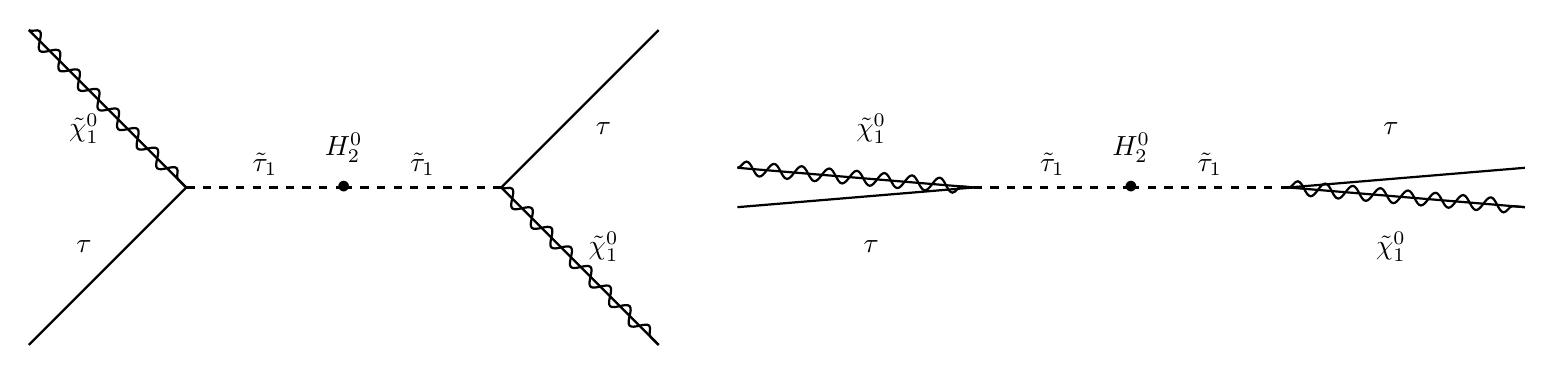
\begin{tikzpicture}
	\begin{scope}[thick] 
	
	\draw[-] (0,3)--(2,1);
	\draw[photon] (0,3)--(2,1);
	\draw[-] (0,-1)--(2,1);
	\draw[-,dashed] (2,1) -- (4,1);
	\draw[-,dashed] (4,1) -- (6,1);
	\draw[-] (6,1)--(8,-1);
	\draw[photon] (6,1)--(8,-1);
	\draw[-] (6,1)--(8,3);
    \node[black] at (4.0,1.0) {{$\bullet$}};
    \node[black] at (4.0,1.5) {{$H_2^0$}};
    \node[black] at (3.0,1.30) {{$\stau_1$}};
    \node[black] at (5.0,1.30) {{$\stau_1$}};
    \node[black] at (7.30,1.75) {{$\tau$}};
    \node[black] at (7.30,0.25) {{$\neut^0_1$}};
    \node[black] at (0.70,1.75) {{$\neut^0_1$}};
    \node[black] at (0.70,0.25) {{$\tau$}};
	
	\draw[-] (9,1.25)--(12,1);
	\draw[photon] (9,1.25)--(12,1);
	\draw[-] (9, 0.75)--(12,1);
	\draw[-,dashed] (12,1) -- (14,1);
	\draw[-,dashed] (14,1) -- (16,1);
	\draw[-] (16,1)--(19,0.75);
	\draw[photon] (16,1)--(19,0.75);
	\draw[-] (16,1)--(19,1.25);
	\node[black] at (14.0,1.0) {{$\bullet$}};
	\node[black] at (14.0,1.5) {{$H_2^0$}};
	\node[black] at (13.0,1.30) {{$\stau_1$}};
	\node[black] at (15.0,1.30) {{$\stau_1$}};
	\node[black] at (17.30,1.75) {{$\tau$}};
	\node[black] at (17.30,0.25) {{$\neut^0_1$}};
	\node[black] at (10.70,1.75) {{$\neut^0_1$}};
	\node[black] at (10.70,0.25) {{$\tau$}};
	
	\end{scope}
	\end{tikzpicture}
    }
    \end{center}
	\caption{On the left a non-boosted decay of the heavy Higgs into staus and its subsecquent decay into a tau lepton and a neutralino. On the right the same decay but this time the decay products are highly boosted, so the neutralino and the tau lepton are almost colinear.}
	\label{fig:nonvsboosted}
\end{figure}

\section{Procedure}
\begin{itemize}
	\item How constrained is the stau? 
	\item Look for two or three benchmark points, BP, in which $m_{H}\gg 2m_{\stau_1}$ and $m_{\neut_1^0}\to 0$ GeV.
	
	(One of the BP can have a heavy Higgs mass of $m_{H}=1750$ GeV ;-) )
	\item Study the production of this heavy Higgs mass (gluon fusion and $b\bar{b}$) and study the main kinematical variables $p_T$, $\met$, $m_{\stau\stau}$, $m_T$, and compare these variables in the case of staus and taus.
	\item Take the analysis of CMS/ATLAS and implement it. Once this is done analyse the case with taus and the case with staus. Do the events in the case of the staus survive? If so, how many of them? Is there a relative large percentage?
\end{itemize}

\end{document}
\begin{figure}
	\begin{center}
		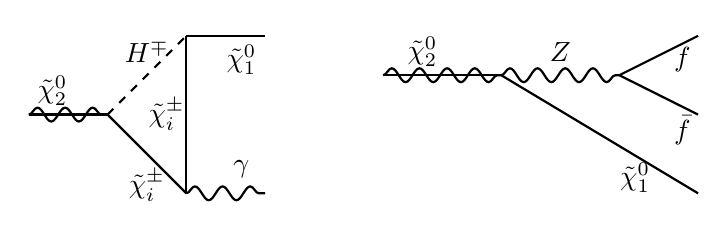
\begin{tikzpicture}
		\begin{scope}[thick] 
		
		\draw[-] (0,0)--(1,0);
		\draw[photon] (0,0)--(1,0);
		\draw[-,dashed] (1,0) -- (2,1);
		\draw[-] (1,0) -- (2,-1);
		\draw[-] (2,-1) -- (2,1);
		\draw[-] (2,1) -- (3,1);
		\draw[photon] (2,-1) -- (3,-1);
		\node[black] at (0.3,0.3) {{$\tilde \chi^0_2$}};
		\node[black] at (2.7,0.7) {{$\tilde \chi^0_1$}};
		\node[black] at (2.7,-0.7) {{$\gamma$}};
		\node[black] at (1.5,0.8) {{$H^\mp$}};
		\node[black] at (1.5,-0.9) {{$\tilde \chi_i^\pm$}};
		\node[black] at (1.75,0) {{$\tilde \chi_i^\pm$}};
		
		
		
		\draw[-] (4.5,0.5) -- (6,0.5);
		\draw[photon] (4.5,0.5) -- (6,0.5);
		\draw[photon] (6,0.5) -- (7.5,0.5);
		\draw[-] (7.5,0.5) -- (8.5,1);
		\draw[-] (7.5,0.5) -- (8.5,0);
		\draw[-] (6,0.5) -- (8.5,-1);
		\node[black] at (5,0.8) {{$\tilde \chi^0_2$}};
		\node[black] at (7.7,-0.8) {{$\tilde \chi^0_1$}};
		\node[black] at (6.75,0.8) {{$Z$}};
		\node[black] at (8.3,0.7) {{$f$}};
		\node[black] at (8.3,-0.2) {{$\bar f$}};
		
		\end{scope}
		\end{tikzpicture}
	\end{center}
	\caption{Radiative and three-body decay of the NLSP in the stealth NMSSM scenario.}
	\label{fig:nmssm_extra_decays}
\end{figure}


\section{Casimir Energy}

Considering the SM + GR compactified on a circle of radius $R$, the effective 3D action for distances larger than $R$, is written as \cite{ArkaniHamed:2007gg}
\begin{eqnarray}
S_{SM+GR}= \int d^3x \sqrt{-g_{(3)}} (2\pi r)\left[\frac{1}{2}M_4^2\mathcal{R}_{(3)}-\frac{1}{4}\frac{R^4}{r^4}V_{\mu\nu}V^{\mu\nu}-M_4^2\left(\frac{\partial R}{R}\right)^2 - \frac{r^2\Lambda_4}{R^2}\right].
\label{eq:action}
\end{eqnarray}
Here $M_4$ is the 4D reduced Planck mass, $M_4=(8\pi G_N)^{-1/2}$ and $\Lambda_4$ is the 4D cosmological constant. In order to study the stabilization of the compact dimension, one must compute quantum corrections to the radion effective potential since there is no classical contribution and the smallness of the cosmological constant. The contribution to the effective potential coming from the cosmological constant can be derived from the last term in Eq.~\ref{eq:action} giving
\begin{equation}
V_{\Lambda}(R)=\frac{2\pi r^3 \Lambda_4}{R^2}.
\end{equation}


The 1-loop corrections to the effective potential of SM particles can be derived from the Casimir energy coming from loops wrapping the circle. These computations are UV insensitive. A particle of mass, $m$ contributes with a term proportional to $\propto e^{-2\pi m R}$ when $R\gg 1/m$. Therefore, only particles with masses lighter than $1/R$ are relevant for the effective potential.
It was shown in Ref.~\cite{ArkaniHamed:2007gg} that the 1-loop Casimir energy contribution of a massless field can be written as
\begin{equation}
\rho(R) = \mp \frac{\pi^2}{90}\frac{1}{(2\pi R)^4},
\end{equation}
where the minus sign stands for bosons and the plus sign for fermions. The effective potential in the dimensionally reduced 3D theory is expressed as 
\begin{equation}
V_C=2\pi  R \rho(R)= \mp \frac{n_0}{720 \pi R^3},
\end{equation}
that is written in the Weyl-rescaled metric as,
\begin{equation}
V_C(R)=2\pi  R \rho(R)= \mp \frac{n_0}{720 \pi}\frac{r^3}{R^6},
\end{equation}
where $n_0$ is the number of degrees of freedom of the particle (two for massless vector bosons, two for Majorana fermions, four for Dirac fermions, etc).

In a general case for a particle of mass, $m$ the Casimir energy density is \cite{ArkaniHamed:2007gg},
\begin{eqnarray}
\rho (R)=\mp\sum_{n=1}^{\infty}\frac{2m^4}{(2\pi)^{2}}\frac{K_{2}(2\pi Rmn)}{(2\pi R m n)^{2}}\cos (n\theta),
\label{eq:casimirrho}
\end{eqnarray}
%\begin{eqnarray}
%\rho (R)=\mp\sum_{n=1}^{\infty}\frac{2m^d}{(2\pi)^{d/2}}\frac{K_{d/2}(2\pi Rmn)}{(2\pi R m n)^{d/2}}\cos (n\theta),
%\label{eq:casimirrho}
%\end{eqnarray}
where $K_i(x)$ is the Bessel function and the $\theta$ angle will be explained in Section~\ref{sec:otherSMvacua}. The massless limit can be achieved taking the argument of the Bessel function in Eq.~\ref{eq:casimirrho} to zero (see Appendix of Ref.~\cite{ArkaniHamed:2007gg}) and reads,
\begin{eqnarray}
\rho(R)=\mp\frac{2}{(2\pi R)^4 \Omega_{3}}{\rm Re}\left[{\rm Li}_4(e^{i\theta}) - \frac{2\pi^2{\rm Li}_{2}(e^{i\theta})}{2}(mR)^2 + \frac{2\pi^4{\rm Li}_{0}(e^{i\theta})}{(d+2)(d+4)} \mathcal{O}(mR)^6\right]
\label{eq:casimirrholimit}
\end{eqnarray}
%\begin{eqnarray}
%\rho(R)=\mp\frac{2}{(2\pi R)^d \Omega_{d-1}}{\rm Re}\left[{\rm Li}_d(e^{i\theta}) - \frac{2\pi^2{\rm Li}_{d-2}(e^i\theta)}{d-2}(mR)^2 + \mathcal{O}(mR)^4\right]
%\label{eq:casimirrholimit}
%\end{eqnarray}
where ${\rm Li}_n(z)=\sum_{k=1}^{\infty}\frac{z^k}{k^n}$ %${\rm Li}_n(z)=\sum_{k=1}^{\infty}\frac{z^k}{k^n}$
and $\Omega_{d-1}=\frac{2\pi^{d/2}}{\Gamma(d/2)}$. Since $\theta$ could be either 0 or $\pi$ then ${\rm Li}_n(1)=\zeta (n)$ and ${\rm Li}_n (-1)=(2^{1-d}-1)\zeta(n)$, where $\zeta(n)$ is the Riemann zeta-function. Computing the terms in Eq.~\ref{eq:casimirrholimit} one gets,
\begin{eqnarray}
\rho (R) = \mp \left[\frac{\pi^2}{90 (2\pi R)^4} - \frac{\pi^2}{6(2\pi R)^4}(mR)^2 + \frac{\pi^2}{48(2\pi R)^4}(mR)^4  + \mathcal{O}(mR)^6\right].
\end{eqnarray}

Summing the contributions of the cosmological constant and the particles the effective potential reads,
\begin{eqnarray}
V(R)= \frac{2\pi r^3 \Lambda_4}{R^2} + \sum_i (2\pi R)n_i\rho_i(R),
\end{eqnarray}
where the sum goes over all the particles in the spectrum and $n_i$ is the number of degrees of freedom of the $i$-th particle. 

Then, one can find a general formula of the potential in terms of the Weyl-rescaled metric when the masses are small,
\begin{eqnarray}
V(R)= \frac{2\pi r^3 \Lambda_4}{R^2} + \sum_i (2\pi R)\frac{r^3}{R^3}n_i\rho_i(R)\simeq  \notag\\ \simeq
\frac{2\pi r^3 \Lambda_4}{R^2} +  \frac{r^3}{R^6}\frac{\pi^2}{(2\pi)^3}\sum_i (-1)^{s_i}n_i  \left[\frac{1}{90} - \frac{1}{6}(m_iR)^2 + \frac{1}{48}(m_iR)^4\right].
\end{eqnarray}
$s_i=0,1$ if the $i$-th state is bosonic or fermionic respectively. Setting the scale $r$ such that $2\pi r=1$ GeV$^{-1}$ the effective potential is written,
\begin{eqnarray}
V(R)= 
\frac{( {\rm GeV}^{-3}) \Lambda_4}{(2\pi R)^2} +  \frac{\pi^2 ( {\rm GeV}^{-3})}{(2\pi R)^6}\sum_i (-1)^{s_i}n_i  \left[\frac{1}{90} - \frac{1}{6}(m_iR)^2 + \frac{1}{48}(m_iR)^4\right].
\label{eq:effpotentialapprox}
\end{eqnarray}


\begin{tcolorbox}[width=\textwidth,colback={white},title={\textbf{Note!}},colbacktitle=myblue,coltitle=white]    
   In the following... \par
   {\color{myblue}$\bullet$} The relation $2\pi r=1$ GeV$^{-1}$ will be taken and the for computation purposes. \par 
   {\color{myblue}$\bullet$} The potential will be calculated using the complete formula of Eq.~\eqref{eq:casimirrho} instead of the approximation formula given in Eq.~\eqref{eq:casimirrholimit}.\par 
   {\color{myblue}$\bullet$} We assume the cosmological constant to be: $\Lambda_4 = 2.6 \cdot 10^{-47}$ GeV$^4$ \cite{Olive:2016xmw}.
\end{tcolorbox} 

\begin{figure}[t]
	\begin{center}
		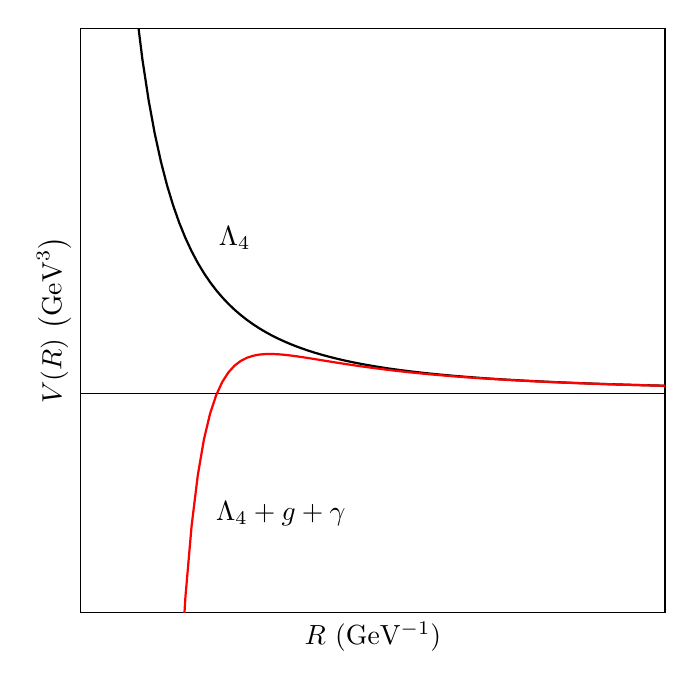
\begin{tikzpicture}
		\begin{axis}	[height=9cm,
		width=9cm,xmin=1.0e+10,   xmax=2.0e+11,
		ymin=-0.6e-69,   ymax=10e-70,title={},
		xlabel=$R$ (GeV$^{-1}$),ylabel=$V(R)$ $\left({\rm GeV}^3\right)$,
		xtick=\empty,
		ytick=\empty 
		]
		\addplot[color=black] coordinates {
			(10000000000,0.0)
			(200000000000,0.0)
		};
		\addplot[color=black, thick] coordinates {
			(10000000000,8.232346170939944e-69)
			(12000000000,5.716907063152738e-69)
			(14000000000,4.2001766178265015e-69)
			(16000000000,3.215760223023416e-69)
			(18000000000,2.5408475836234396e-69)
			(20000000000,2.058086542734986e-69)
			(22000000000,1.7008979692024676e-69)
			(24000000000,1.4292267657881845e-69)
			(26000000000,1.2178026880088674e-69)
			(28000000000,1.0500441544566254e-69)
			(30000000000,9.147051301044382e-70)
			(32000000000,8.03940055755854e-70)
			(34000000000,7.121406722266387e-70)
			(36000000000,6.352118959058599e-70)
			(38000000000,5.701070755498576e-70)
			(40000000000,5.145216356837465e-70)
			(42000000000,4.6668629086961134e-70)
			(44000000000,4.252244923006169e-70)
			(46000000000,3.890522765094491e-70)
			(48000000000,3.5730669144704614e-70)
			(50000000000,3.292938468375977e-70)
			(52000000000,3.0445067200221684e-70)
			(54000000000,2.8231639818038214e-70)
			(56000000000,2.6251103861415634e-70)
			(58000000000,2.4471897059869036e-70)
			(60000000000,2.2867628252610954e-70)
			(62000000000,2.1416093056555525e-70)
			(64000000000,2.009850139389635e-70)
			(66000000000,1.8898866324471865e-70)
			(68000000000,1.7803516805665968e-70)
			(70000000000,1.6800706471306005e-70)
			(72000000000,1.5880297397646498e-70)
			(74000000000,1.5033502868772723e-70)
			(76000000000,1.425267688874644e-70)
			(78000000000,1.3531140977876304e-70)
			(80000000000,1.2863040892093663e-70)
			(82000000000,1.2243227499910684e-70)
			(84000000000,1.1667157271740284e-70)
			(86000000000,1.1130808776284401e-70)
			(88000000000,1.0630612307515423e-70)
			(90000000000,1.0163390334493759e-70)
			(92000000000,9.726306912736227e-71)
			(94000000000,9.31682454837024e-71)
			(96000000000,8.932667286176153e-71)
			(98000000000,8.571789015972455e-71)
			(100000000000,8.232346170939943e-71)
			(102000000000,7.91267413585154e-71)
			(104000000000,7.611266800055421e-71)
			(106000000000,7.32675878510141e-71)
			(108000000000,7.0579099545095536e-71)
			(110000000000,6.803591876809872e-71)
			(112000000000,6.5627759653539085e-71)
			(114000000000,6.334523061665084e-71)
			(116000000000,6.117974264967259e-71)
			(118000000000,5.9123428403762886e-71)
			(120000000000,5.7169070631527385e-71)
			(122000000000,5.531003877277577e-71)
			(124000000000,5.354023264138881e-71)
			(126000000000,5.1854032318845706e-71)
			(128000000000,5.0246253484740875e-71)
			(130000000000,4.8712107520354695e-71)
			(132000000000,4.724716581117966e-71)
			(134000000000,4.584732775083506e-71)
			(136000000000,4.450879201416492e-71)
			(138000000000,4.322803072327213e-71)
			(140000000000,4.200176617826501e-71)
			(142000000000,4.082694986580016e-71)
			(144000000000,3.9700743494116244e-71)
			(146000000000,3.862050183402113e-71)
			(148000000000,3.758375717193181e-71)
			(150000000000,3.658820520417753e-71)
			(152000000000,3.56316922218661e-71)
			(154000000000,3.4712203453111587e-71)
			(156000000000,3.382785244469076e-71)
			(158000000000,3.297687137854488e-71)
			(160000000000,3.2157602230234157e-71)
			(162000000000,3.1368488686709125e-71)
			(164000000000,3.060806874977671e-71)
			(166000000000,2.9874967959573027e-71)
			(168000000000,2.916789317935071e-71)
			(170000000000,2.848562688906555e-71)
			(172000000000,2.7827021940711003e-71)
			(174000000000,2.7190996733187815e-71)
			(176000000000,2.6576530768788556e-71)
			(178000000000,2.598266055718957e-71)
			(180000000000,2.5408475836234396e-71)
			(182000000000,2.485311608181362e-71)
			(184000000000,2.431576728184057e-71)
			(186000000000,2.3795658951728362e-71)
			(188000000000,2.32920613709256e-71)
			(190000000000,2.28042830219943e-71)
			(192000000000,2.2331668215440383e-71)
			(194000000000,2.187359488505671e-71)
			(196000000000,2.1429472539931137e-71)
			(198000000000,2.099874036052429e-71)
			(200000000000,2.0580865427349858e-71)
		};
		\addplot[color=red, thick] coordinates {
			%(24000000000,-3.5876075813752953e-68)
			%(26000000000,-2.186018457390031e-68)
			%(28000000000,-1.3744099417958538e-68)
			(30000000000,-8.864656109306795e-69)
			(32000000000,-5.835602322292362e-69)
			(34000000000,-3.9027829191950403e-69)
			(36000000000,-2.639876396399536e-69)
			(38000000000,-1.7976461527862974e-69)
			(40000000000,-1.2259945614673249e-69)
			(42000000000,-8.321136935399501e-70)
			(44000000000,-5.5725152582750364e-70)
			(46000000000,-3.63420906649998e-70)
			(48000000000,-2.2558866135828415e-70)
			(50000000000,-1.2697203114837279e-70)
			(52000000000,-5.614287896511409e-71)
			(54000000000,-5.208499909529122e-72)
			(56000000000,3.135254529516941e-71)
			(58000000000,5.74481749103206e-71)
			(60000000000,7.587376316030903e-71)
			(62000000000,8.864817044702165e-71)
			(64000000000,9.724216428196013e-71)
			(66000000000,1.027356246161868e-70)
			(68000000000,1.0592698694069595e-70)
			(70000000000,1.0741025264044755e-70)
			(72000000000,1.0762971940919317e-70)
			(74000000000,1.0691923960478897e-70)
			(76000000000,1.0553062469471198e-70)
			(78000000000,1.0365436278025937e-70)
			(80000000000,1.0143484334045114e-70)
			(82000000000,9.898162403103084e-71)
			(84000000000,9.637782296100345e-71)
			(86000000000,9.368640779379205e-71)
			(88000000000,9.095493529190234e-71)
			(90000000000,8.821914169965468e-71)
			(92000000000,8.55056756404959e-71)
			(94000000000,8.283418746391493e-71)
			(96000000000,8.021893297417825e-71)
			(98000000000,7.767000884637237e-71)
			(100000000000,7.519430736586863e-71)
			(102000000000,7.279625632227168e-71)
			(104000000000,7.047839376668966e-71)
			(106000000000,6.824181535212077e-71)
			(108000000000,6.608652301244067e-71)
			(110000000000,6.4011696997845935e-71)
			(112000000000,6.201590819542991e-71)
			(114000000000,6.00972838013749e-71)
			(116000000000,5.825363646704181e-71)
			(118000000000,5.6482564787248725e-71)
			(120000000000,5.478153126643675e-71)
			(122000000000,5.314792256148537e-71)
			(124000000000,5.157909576453673e-71)
			(126000000000,5.007241368453904e-71)
			(128000000000,4.86252714588502e-71)
			(130000000000,4.723511633559251e-71)
			(132000000000,4.589946208260885e-71)
			(134000000000,4.461589917620549e-71)
			(136000000000,4.338210168422799e-71)
			(138000000000,4.219583156941829e-71)
			(140000000000,4.105494098963044e-71)
			(142000000000,3.995737305294653e-71)
			(144000000000,3.890116139150262e-71)
			(146000000000,3.7884428842806675e-71)
			(148000000000,3.690538546751089e-71)
			(150000000000,3.5962326084855213e-71)
			(152000000000,3.5053627468854344e-71)
			(154000000000,3.417774531780912e-71)
			(156000000000,3.333321108533914e-71)
			(158000000000,3.251862874163495e-71)
			(160000000000,3.173267151803907e-71)
			(162000000000,3.097407867561185e-71)
			(164000000000,3.0241652328400523e-71)
			(166000000000,2.9534254344213125e-71)
			(168000000000,2.885080333940697e-71)
			(170000000000,2.819027177921456e-71)
			(172000000000,2.7551683191194566e-71)
			(174000000000,2.6934109496303904e-71)
			(176000000000,2.6336668459675246e-71)
			(178000000000,2.5758521261317346e-71)
			(180000000000,2.519887018552685e-71)
			(182000000000,2.4656956426721704e-71)
			(184000000000,2.4132058008608283e-71)
			(186000000000,2.3623487813019813e-71)
			(188000000000,2.313059171436642e-71)
			(190000000000,2.265274681538079e-71)
			(192000000000,2.2189359779696895e-71)
			(194000000000,2.1739865256739654e-71)
			(196000000000,2.130372439441001e-71)
			(198000000000,2.088042343510792e-71)
			(200000000000,2.046947239073219e-71)
		};
		\node[anchor=south] at (axis cs:60000000000,3.67664047370961e-70) {$\Lambda_4$};
		\node[anchor=south] at (axis cs:75000000000,-3.9027829191950403e-70) {$\Lambda_4 + g + \gamma$};
		\end{axis}%
		\end{tikzpicture}%
		\caption{\footnotesize Effective potential as a function of the radion field, $R$, for the cosmological constant (black) and the sum of the cosmological constant, graviton and photon contributions (red).}
		\label{fig:casimirmassless}
	\end{center}
\end{figure}

\section{Massless particles contribution}

The first contribution of SM particles are those coming from massless ones, since they are not exponentially suppressed. Within the SM, the only massless particles are the graviton and the photon. If we only take into account these contribution the effective potential reads,
\begin{eqnarray}
V (R)= \frac{2\pi r^3 \Lambda_4}{R^2} - 4\left(\frac{r^3}{720\pi R^6}\right),
\label{eq:masslesscontri}
\end{eqnarray}
where the number four comes from the sum of the degrees of freedom of the massless particles, two for the photon and two for the graviton. In Fig.~\ref{fig:casimirmassless} the contributions from the massless states and the cosmological constant are depicted. The contribution of the cosmological constant is shown as a black line. Only this contribution does not present any minimum. If we include the massless states, the graviton and the photon, we see that the effective potential, red line, drops for small $R$. In this case there is no minimum. It is clear that the negative sign of the bosonic massless states pushes the effective potential to negative values for small radius due to the sixth power of the radion field, $R^{-6}$ compared with the squared of the cosmological constant, $R^2$, that is important for larger values of $R$. However a maximum appears due to the different behaviours of the two contributions. Deriving Eq.~\eqref{eq:masslesscontri} with respect to $R$, one obtain that the maximum is achieved for a value $R_{max}$,
\begin{equation}
R_{max}=\left(\frac{1}{120\pi^2\Lambda_4}\right)^{1/4}.
\end{equation}

\begin{tcolorbox}[width=\textwidth,colback={white},title={\textbf{Note!}},colbacktitle=myblue,coltitle=white]    
This result is the same as the one obtained in Ref.~\cite{ArkaniHamed:2007gg}.
\end{tcolorbox} 

Using the value of the cosmological constant, $\Lambda_4=2.6 \cdot 10^{-47}$ GeV$^4$ \cite{Olive:2016xmw},
\begin{eqnarray}
R_{max}=\left(\frac{1}{120\pi^2\Lambda_4}\right)^{1/4}=7.55\cdot 10^{10}\,{\rm GeV}^{-1},
\end{eqnarray}
and the associated mass parameter here will be,
\begin{eqnarray}
M_{m}=\frac{1}{2\pi R_{max}}=2.11\cdot 10^{-3}\,{\rm eV}.
\end{eqnarray}

\begin{figure}[t]
	\begin{center}
		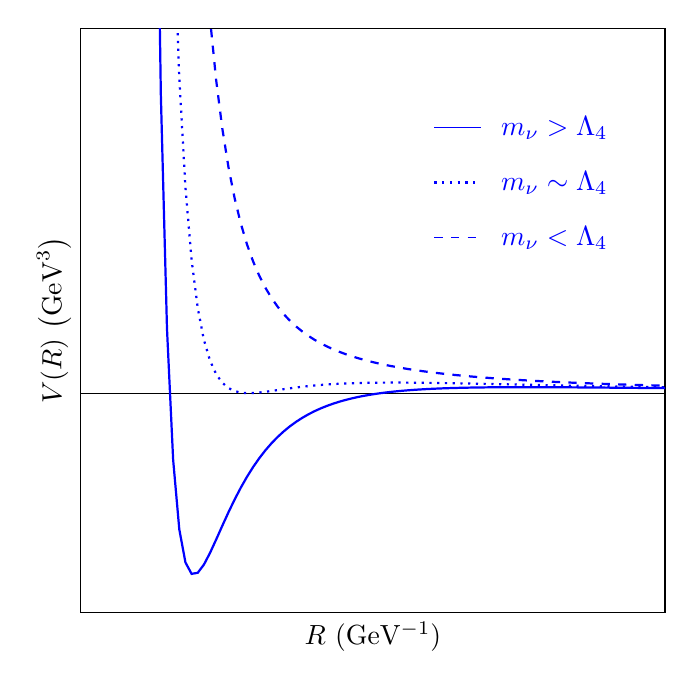
\begin{tikzpicture}
		\begin{axis}	[height=9cm,
		width=9cm,xmin=1.0e+10,   xmax=2.0e+11,
		ymin=-0.6e-69,   ymax=10e-70,title={},
		xlabel=$R$ (GeV$^{-1}$),ylabel=$V(R)$ $\left({\rm GeV}^3\right)$,
		xtick=\empty,
		ytick=\empty 
		]
		\addplot[color=black] coordinates {
			(10000000000,0.0)
			(200000000000,0.0)
		};
		\addplot[color=blue, dotted, thick] coordinates {
			(22000000000,9.823741326099609e-68)
			(24000000000,5.5408268632344526e-68)
			(26000000000,3.239474649043029e-68)
			(28000000000,1.950192728966029e-68)
			(30000000000,1.202273928430828e-68)
			(32000000000,7.5550692388265e-69)
			(34000000000,4.819730022503122e-69)
			(36000000000,3.110017953597945e-69)
			(38000000000,2.022826441624199e-69)
			(40000000000,1.3217034272745273e-69)
			(42000000000,8.645027516143315e-70)
			(44000000000,5.639005892689935e-70)
			(46000000000,3.6521588249723394e-70)
			(48000000000,2.3362469127483543e-70)
			(50000000000,1.466163959389648e-70)
			(52000000000,8.94483538495701e-71)
			(54000000000,5.235473225280627e-71)
			(56000000000,2.88027746504637e-71)
			(58000000000,1.4386266704076694e-71)
			(60000000000,6.113300969046415e-72)
			(62000000000,1.941872245320592e-72)
			(64000000000,4.73489938858586e-73)
			(66000000000,7.48875951093137e-73)
			(68000000000,2.1104157531575054e-72)
			(70000000000,4.108746211842502e-72)
			(72000000000,6.438825178589507e-72)
			(74000000000,8.895878547007926e-72)
			(76000000000,1.1344864110596188e-71)
			(78000000000,1.3699198573339058e-71)
			(80000000000,1.590587741244748e-71)
			(82000000000,1.793503458372313e-71)
			(84000000000,1.9772602975551453e-71)
			(86000000000,2.1415150960126265e-71)
			(88000000000,2.286625243616647e-71)
			(90000000000,2.4133941146384556e-71)
			(92000000000,2.5228933580400663e-71)
			(94000000000,2.6163397566449457e-71)
			(96000000000,2.6950108525498655e-71)
			(98000000000,2.7601880960511947e-71)
			(100000000000,2.8131194967050146e-71)
			(102000000000,2.8549960411658738e-71)
			(104000000000,2.886937771282651e-71)
			(106000000000,2.9099865806168264e-71)
			(108000000000,2.925103622869286e-71)
			(110000000000,2.9331698262834966e-71)
			(112000000000,2.9349884407153265e-71)
			(114000000000,2.9312888560808025e-71)
			(116000000000,2.9227311560474577e-71)
			(118000000000,2.9099110332552283e-71)
			(120000000000,2.893364809366715e-71)
			(122000000000,2.873574387341073e-71)
			(124000000000,2.8509720235261627e-71)
			(126000000000,2.8259448500120737e-71)
			(128000000000,2.7988391079390252e-71)
			(130000000000,2.7699640735643973e-71)
			(132000000000,2.7395956733903205e-71)
			(134000000000,2.707979794376468e-71)
			(136000000000,2.6753353015574433e-71)
			(138000000000,2.6418567792324133e-71)
			(140000000000,2.6077170140131494e-71)
			(142000000000,2.573069238927385e-71)
			(144000000000,2.53804915785673e-71)
			(146000000000,2.5027767691169807e-71)
			(148000000000,2.4673580061611387e-71)
			(150000000000,2.4318862123432365e-71)
			(152000000000,2.39644346552413e-71)
			(154000000000,2.361101767098606e-71)
			(156000000000,2.325924108824204e-71)
			(158000000000,2.2909654296679835e-71)
			(160000000000,2.2562734737783068e-71)
			(162000000000,2.221889559646665e-71)
			(164000000000,2.18784926955581e-71)
			(166000000000,2.1541830675171915e-71)
			(168000000000,2.1209168530822553e-71)
			(170000000000,2.088072457666053e-71)
			(172000000000,2.055668089344252e-71)
			(174000000000,2.0237187314716707e-71)
			(176000000000,1.9922364999171957e-71)
			(178000000000,1.9612309632117466e-71)
			(180000000000,1.930709429457956e-71)
			(182000000000,1.9006772034481033e-71)
			(184000000000,1.871137817076175e-71)
			(186000000000,1.842093235806766e-71)
			(188000000000,1.8135440436742217e-71)
			(190000000000,1.7854896090264578e-71)
			(192000000000,1.757928232996302e-71)
			(194000000000,1.7308572824760012e-71)
			(196000000000,1.7042733091853582e-71)
			(198000000000,1.6781721562583084e-71)
			(200000000000,1.6525490536247017e-71)
		};
		\addplot[color=blue, dashed, thick] coordinates {
			(24000000000,7.603983192487046e-68)
			(26000000000,4.737377721182723e-68)
			(28000000000,3.0638331299286955e-68)
			(30000000000,2.04734276089269e-68)
			(32000000000,1.4083024811852285e-68)
			(34000000000,9.941987855069995e-69)
			(36000000000,7.185388480516651e-69)
			(38000000000,5.305613532222168e-69)
			(40000000000,3.9955540299858893e-69)
			(42000000000,3.064286259688734e-69)
			(44000000000,2.390176528556858e-69)
			(46000000000,1.8939986428283433e-69)
			(48000000000,1.5230973970577067e-69)
			(50000000000,1.2418256028095388e-69)
			(52000000000,1.0256377739368786e-69)
			(54000000000,8.573661943602047e-70)
			(56000000000,7.248280252521302e-70)
			(58000000000,6.1926056197543e-70)
			(60000000000,5.342813212577106e-70)
			(62000000000,4.651864508026225e-70)
			(64000000000,4.0847071325297024e-70)
			(66000000000,3.614947405017824e-70)
			(68000000000,3.222515302885871e-70)
			(70000000000,2.8920068885828505e-70)
			(72000000000,2.6114948311100856e-70)
			(74000000000,2.3716660685360374e-70)
			(76000000000,2.1651905727296923e-70)
			(78000000000,1.986255037757704e-70)
			(80000000000,1.8302154008190763e-70)
			(82000000000,1.6933357693525884e-70)
			(84000000000,1.5725907223020162e-70)
			(86000000000,1.4655144770094796e-70)
			(88000000000,1.37008498641658e-70)
			(90000000000,1.284634266355034e-70)
			(92000000000,1.20777856101095e-70)
			(94000000000,1.1383636152327735e-70)
			(96000000000,1.075421526369281e-70)
			(98000000000,1.0181365278642892e-70)
			(100000000000,9.658177039646098e-71)
			(102000000000,9.178771143100286e-71)
			(104000000000,8.738121646828329e-71)
			(106000000000,8.331913284880078e-71)
			(108000000000,7.956425261040526e-71)
			(110000000000,7.608436230860429e-71)
			(112000000000,7.285146256975742e-71)
			(114000000000,6.984112424720271e-71)
			(116000000000,6.703195501493414e-71)
			(118000000000,6.440515563679121e-71)
			(120000000000,6.194414936170865e-71)
			(122000000000,5.963427119535657e-71)
			(124000000000,5.746250639509298e-71)
			(126000000000,5.541726958745904e-71)
			(128000000000,5.348821753652223e-71)
			(130000000000,5.166608988987907e-71)
			(132000000000,4.994257326832128e-71)
			(134000000000,4.83101849000942e-71)
			(136000000000,4.67621726740388e-71)
			(138000000000,4.5292429030979794e-71)
			(140000000000,4.389541655553416e-71)
			(142000000000,4.2566103491507426e-71)
			(144000000000,4.1299907699343486e-71)
			(146000000000,4.009264781645003e-71)
			(148000000000,3.894050058077363e-71)
			(150000000000,3.783996344282217e-71)
			(152000000000,3.678782172788961e-71)
			(154000000000,3.578111972371652e-71)
			(156000000000,3.4817135163394e-71)
			(158000000000,3.3893356652364743e-71)
			(160000000000,3.300746365462433e-71)
			(162000000000,3.2157308708903673e-71)
			(164000000000,3.1340901592529087e-71)
			(166000000000,3.0556395190292833e-71)
			(168000000000,2.980207285923819e-71)
			(170000000000,2.907633710876753e-71)
			(172000000000,2.8377699439743877e-71)
			(174000000000,2.7704771206955636e-71)
			(176000000000,2.7056255387015176e-71)
			(178000000000,2.6430939148934023e-71)
			(180000000000,2.582768713764949e-71)
			(182000000000,2.5245435391997457e-71)
			(184000000000,2.468318582830514e-71)
			(186000000000,2.414000122914546e-71)
			(188000000000,2.361500068404396e-71)
			(190000000000,2.3107355435221326e-71)
			(192000000000,2.261628508692736e-71)
			(194000000000,2.214105414169082e-71)
			(196000000000,2.1680968830973392e-71)
			(198000000000,2.123537421135703e-71)
			(200000000000,2.080365150058519e-71)
		};
		\addplot[color=blue, thick] coordinates {
			(22000000000,8.180349760672628e-68)
			(24000000000,4.3804827318004045e-68)
			(26000000000,2.3970358020342963e-68)
			(28000000000,1.3238678666842605e-68)
			(30000000000,7.26996972195442e-69)
			(32000000000,3.8836678854609575e-69)
			(34000000000,1.9389101197940527e-69)
			(36000000000,8.179801631109374e-70)
			(38000000000,1.765471842967984e-70)
			(40000000000,-1.821025670639985e-70)
			(42000000000,-3.726821615348406e-70)
			(44000000000,-4.63219139122869e-70)
			(46000000000,-4.9459007550807654e-70)
			(48000000000,-4.915903908714445e-70)
			(50000000000,-4.693425393420953e-70)
			(52000000000,-4.370759255308879e-70)
			(54000000000,-4.003934732754917e-70)
			(56000000000,-3.626502642756416e-70)
			(58000000000,-3.258023699115884e-70)
			(60000000000,-2.909347966780699e-70)
			(62000000000,-2.585924946983266e-70)
			(64000000000,-2.2898909464648776e-70)
			(66000000000,-2.021389716324847e-70)
			(68000000000,-1.7794082816615937e-70)
			(70000000000,-1.562304185322902e-70)
			(72000000000,-1.3681353672684842e-70)
			(74000000000,-1.1948634640280385e-70)
			(76000000000,-1.0404758947236635e-70)
			(78000000000,-9.030559735366497e-71)
			(80000000000,-7.808199723371037e-71)
			(82000000000,-6.721334105532208e-71)
			(84000000000,-5.75514540962718e-71)
			(86000000000,-4.896301936747224e-71)
			(88000000000,-4.132873058832493e-71)
			(90000000000,-3.4542226290082837e-71)
			(92000000000,-2.850893879493125e-71)
			(94000000000,-2.314494023148529e-71)
			(96000000000,-1.8375834108643845e-71)
			(98000000000,-1.4135719191542587e-71)
			(100000000000,-1.0366238488016124e-71)
			(102000000000,-7.01571739956433e-72)
			(104000000000,-4.038389748452117e-72)
			(106000000000,-1.3937072845171e-72)
			(108000000000,9.542733831742395e-73)
			(110000000000,3.037433216003287e-72)
			(112000000000,4.88406947427169e-72)
			(114000000000,6.519317482691977e-72)
			(116000000000,7.96552177199551e-72)
			(118000000000,9.242562434526953e-72)
			(120000000000,1.0368141990722374e-71)
			(122000000000,1.1358037521433694e-71)
			(124000000000,1.222632230128367e-71)
			(126000000000,1.2985560683464293e-71)
			(128000000000,1.3646979542806104e-71)
			(130000000000,1.4220619183504248e-71)
			(132000000000,1.4715466259929597e-71)
			(134000000000,1.5139570941298456e-71)
			(136000000000,1.5500150270617133e-71)
			(138000000000,1.5803679421888197e-71)
			(140000000000,1.60559723436232e-71)
			(142000000000,1.6262253087908307e-71)
			(144000000000,1.6427218959477423e-71)
			(146000000000,1.6555096475577115e-71)
			(148000000000,1.6649691002248156e-71)
			(150000000000,1.6714430823666191e-71)
			(152000000000,1.6752406306306138e-71)
			(154000000000,1.67664047370961e-71)
			(156000000000,1.6758941342804292e-71)
			(158000000000,1.6732286935257299e-71)
			(160000000000,1.6688492572398203e-71)
			(162000000000,1.6629411577598778e-71)
			(164000000000,1.6556719218117777e-71)
			(166000000000,1.6471930307348869e-71)
			(168000000000,1.63764149638336e-71)
			(170000000000,1.6271412732326015e-71)
			(172000000000,1.6158045247967613e-71)
			(174000000000,1.60373276034122e-71)
			(176000000000,1.5910178560141245e-71)
			(178000000000,1.5777429728893035e-71)
			(180000000000,1.5639833829800347e-71)
			(182000000000,1.5498072130238081e-71)
			(184000000000,1.5352761147303503e-71)
			(186000000000,1.5204458692096709e-71)
			(188000000000,1.5053669324371294e-71)
			(190000000000,1.4900849278540738e-71)
			(192000000000,1.4746410915329116e-71)
			(194000000000,1.459072674743601e-71)
			(196000000000,1.4434133082350176e-71)
			(198000000000,1.4276933320810519e-71)
			(200000000000,1.4119400945305375e-71)
		};
		\addplot[color=blue] coordinates {
			(125000000000,7.27664047370961e-70)
			(140000000000,7.27664047370961e-70)
		};
		\addplot[color=blue, dotted, thick] coordinates {
			(125000000000,5.77664047370961e-70)
			(140000000000,5.77664047370961e-70)
		};
		\addplot[color=blue, dashed] coordinates {
			(125000000000,4.27664047370961e-70)
			(140000000000,4.27664047370961e-70)
		};
		\node[anchor=south, blue] at (axis cs:164000000000,6.67664047370961e-70) {$m_\nu > \Lambda_4$};
		\node[anchor=south, blue] at (axis cs:164000000000,5.17664047370961e-70) {$m_\nu \sim \Lambda_4$};
		\node[anchor=south, blue] at (axis cs:164000000000,3.67664047370961e-70) {$m_\nu < \Lambda_4$};
		\end{axis}%
		\end{tikzpicture}%
		\caption{\footnotesize Different effective potentials depending on the sum of the neutrino masses. If the sum of the neutrino masses is greater than the 4D cosmological constant an AdS vacuum is formed(full line), when the sum is of the same order of the cosmological constant a dS vacuum is formed (dotted line) and no vacuum is achieved when the neutrinos are lighter (dashed line).}
		\label{fig:effectiveneutrinos}
	\end{center}
\end{figure}


\section{Neutrino contribution}
\label{sec:neutrinos}
The next-to the massless particles in the SM are the neutrinos. We do not know the exact masses of the neutrinos, however we know the differences between them. Furthermore, we have some upper bounds to the sum of the masses of the neutrinos. However, as neutrinos have non-zero masses they will be important for the effective potential when $1/R$ approaches their mass. As we saw in Fig.~\ref{fig:casimirmassless} the contribution of the massless bosonic particles makes the effective potential to drop for small $R$. However, when $1/R$ approaches the neutrino mass scale the contribution from them is important. In fact, as they are fermions their contribution has opposite sign with respect to the one of the massless bosonic states\footnote{This is only true if one considers periodic boundary conditions for fermions.}. This fact makes the effective potential to have positive values. In this case, there is the possibility that a minimum is developed, depending on the neutrino masses. There are three possibilities (see also Fig.~\ref{fig:effectiveneutrinos}): 
\begin{itemize}
	\item [a)]  \underline{$m_\nu < \Lambda_4$}: No vacuum is created.
	\item [b)]  \underline{$m_\nu \sim \Lambda_4$}: A dS vacuum is created.
	\item [c)] \underline{ $m_\nu > \Lambda_4$}: An AdS vacuum is created.
\end{itemize}
The last possibility, when $m_\nu > \Lambda_4$ and an AdS vacuum is created should be forbidden by WGC arguments \cite{Ooguri:2016pdq}. In that sense, the WGC could impose stringent bounds on the mass of the neutrinos compared with the upper bounds coming from the experimental side. 

Nowadays we do not know the absolute masses of the neutrinos, nonetheless we are able to measure the difference in masses between them. According the PDG \cite{Olive:2016xmw} the atmospheric and solar difference in masses are,
\begin{eqnarray}
\Delta m_{21}^2 = (7.53\pm 0.18)\times 10^{-5}\,\, {\rm eV}^2,\\
\Delta m_{32}^2 = (2.44\, \pm 0.06)\times 10^{-3}\,\, {\rm eV}^2 \,\,{\rm (NH)},\\
\Delta m_{32}^2 =(2.51\pm 0.06)\times 10^{-3}\,\, {\rm eV}^2 \,\,{\rm (IH)}.
\end{eqnarray}
\begin{figure}
  \begin{center}
    \begin{tikzpicture}[scale=0.5]
    \begin{scope} % Energy levels
        \draw (1,0) node[left] {$\nu_1$} -- 
            ++(6,0) node[right] {};
        \draw (1,2) node[left] {$\nu_2$} -- 
            ++(6,0) node[right] {};
        \draw (1,6) node[left] {$\nu_3$} -- 
            ++(6,0) node[right] {};
    \end{scope}
    \begin{scope}[color=myblue, thick] % X-rays in, electron out
        \draw[<->] (1.2,0.0) -- (1.2,2);
        \filldraw (1.0,1) circle (0.0) node[right=5] {$\Delta m_{21}^2$};
        \draw[<->] (4,2.0) -- (4,6);
        \filldraw (4.0,4) circle (0.0) node[right=5] {$\Delta m_{32}^2$};
    \end{scope}
    \end{tikzpicture}
    \hspace{2cm}
       \begin{tikzpicture}[scale=0.5]
        \begin{scope} % Energy levels
            \draw (1,0) node[left] {$\nu_3$} -- 
                ++(6,0) node[right] {};
            \draw (1,4) node[left] {$\nu_1$} -- 
                ++(6,0) node[right] {};
            \draw (1,6) node[left] {$\nu_2$} -- 
                ++(6,0) node[right] {};
        \end{scope}
        \begin{scope}[color=myblue, thick] % X-rays in, electron out
            \draw[<->] (1.2,0.0) -- (1.2,6);
            \filldraw (0.9,3) circle (0.0) node[right=5] {$\Delta m_{32}^2$};
            \draw[<->] (4,4.0) -- (4,6);
            \filldraw (4.0,5) circle (0.0) node[right=5] {$\Delta m_{21}^2$};
        \end{scope}
            
        \end{tikzpicture}
		\caption{\footnotesize Normal Hierarchy (NH) and Inverted Hierarchy (IH) for neutrino masses. We will use this convention that is the one used by the PDG~\cite{Olive:2016xmw}.}
		\label{fig:normalinverted}
	\end{center}
\end{figure}
\begin{figure}[t]
	\begin{center}
		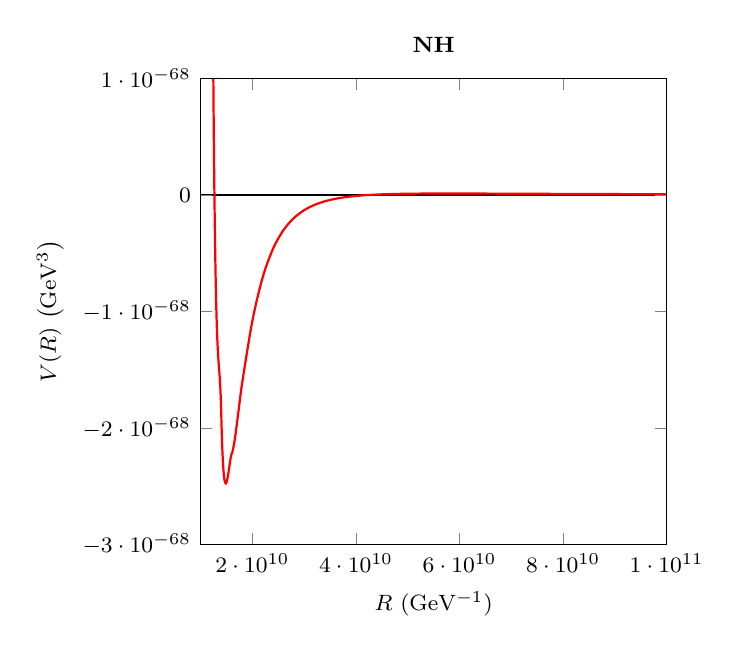
\begin{tikzpicture}
		\begin{axis}	
		[height=7.5cm,
		width=7.5cm, axis on top, ticklabel style = {font=\footnotesize},xmin=1.0e+10,   xmax=1.0e+11,
		ymin=-3.0e-68,   ymax=1.0e-68,title={\footnotesize \textbf{NH}},
		xlabel={\footnotesize $R$ (GeV$^{-1}$)},ylabel={\footnotesize $V(R)$ $\left({\rm GeV}^3\right)$},
		%xtick=\empty,
		%ytick=\empty 
		scaled x ticks=false,
        scaled y ticks=false,
		]
		\addplot[color=black] coordinates {
			(2.0e+8,0.0)
			(200000000000,0.0)
		};
		\addplot[color=red, thick, smooth] coordinates {
        (10000000000,5.437967991933292e-67)
        (12000000000,5.148563693546245e-68)
        (14000000000,-1.9119205737391662e-68)
        (16000000000,-2.221869008814689e-68)
        (18000000000,-1.619207417219074e-68)
        (20000000000,-1.0781634104488958e-68)
        (22000000000,-7.03742728352383e-69)
        (24000000000,-4.5937374521897455e-69)
        (26000000000,-3.0131308852496974e-69)
        (28000000000,-1.9832565800890723e-69)
        (30000000000,-1.3036917571661558e-69)
        (32000000000,-8.491660615037272e-70)
        (34000000000,-5.4132861924311515e-70)
        (36000000000,-3.3062440964651606e-70)
        (38000000000,-1.852315821525575e-70)
        (40000000000,-8.437940588606137e-71)
        (42000000000,-1.4290330886101669e-71)
        (44000000000,3.4314898866992953e-71)
        (46000000000,6.777467130161464e-71)
        (48000000000,9.047456943852749e-71)
        (50000000000,1.0548439767114595e-70)
        (52000000000,1.149753169087112e-70)
        (54000000000,1.2049703974647695e-70)
        (56000000000,1.2316458912579598e-70)
        (58000000000,1.2378575066305835e-70)
        (60000000000,1.2294909242152083e-70)
        (62000000000,1.2108542439689248e-70)
        (64000000000,1.1851115020021678e-70)
        (66000000000,1.1545913344297873e-70)
        (68000000000,1.1210086459595212e-70)
        (70000000000,1.0856250660718419e-70)
        (72000000000,1.0493659407326192e-70)
        (74000000000,1.012906199532985e-70)
        (76000000000,9.767337588105189e-71)
        (78000000000,9.411965926210324e-71)
        (80000000000,9.065378489197744e-71)
        (82000000000,8.729221599918852e-71)
        (84000000000,8.404554289437847e-71)
        (86000000000,8.091997568894304e-71)
        (88000000000,7.791847329349306e-71)
        (90000000000,7.504159895098319e-71)
        (92000000000,7.2288169329654225e-71)
        (94000000000,6.965574720790076e-71)
        (96000000000,6.714101527848592e-71)
        (98000000000,6.474005934611249e-71)
        (100000000000,6.24485823087301e-71)
        (102000000000,6.026206516677203e-71)
        (104000000000,5.8175887439264604e-71)
        (106000000000,5.618541644987686e-71)
        (108000000000,5.4286072737257755e-71)
        (110000000000,5.247337716453538e-71)
        (112000000000,5.0742984021246075e-71)
        (114000000000,4.909070342974312e-71)
        (116000000000,4.751251561460352e-71)
        (118000000000,4.6004579013272225e-71)
        (120000000000,4.456323375819358e-71)
        (122000000000,4.318500171404885e-71)
        (124000000000,4.186658398498633e-71)
        (126000000000,4.06048565980462e-71)
        (128000000000,3.939686490670623e-71)
        (130000000000,3.823981713215999e-71)
        (132000000000,3.713107736155158e-71)
        (134000000000,3.6068158245735577e-71)
        (136000000000,3.5048713579420064e-71)
        (138000000000,3.4070530900070182e-71)
        (140000000000,3.313152420581455e-71)
        (142000000000,3.222972686456036e-71)
        (144000000000,3.1363284764829695e-71)
        (146000000000,3.0530449742108856e-71)
        (148000000000,2.9729573301678565e-71)
        (150000000000,2.8959100649123805e-71)
        (152000000000,2.821756503234393e-71)
        (154000000000,2.750358239337746e-71)
        (156000000000,2.681584632430943e-71)
        (158000000000,2.615312331862129e-71)
        (160000000000,2.5514248307318417e-71)
        (162000000000,2.489812046782788e-71)
        (164000000000,2.4303699292842068e-71)
        (166000000000,2.373000090586666e-71)
        (168000000000,2.31760946101171e-71)
        (170000000000,2.264109965751934e-71)
        (172000000000,2.212418222484791e-71)
        (174000000000,2.1624552584430117e-71)
        (176000000000,2.114146245732368e-71)
        (178000000000,2.0674202537406573e-71)
        (180000000000,2.0222100175382257e-71)
        (182000000000,1.9784517212282675e-71)
        (184000000000,1.936084795263346e-71)
        (186000000000,1.895051726802166e-71)
        (188000000000,1.8552978822368258e-71)
        (190000000000,1.816771341075179e-71)
        (192000000000,1.7794227404151205e-71)
        (194000000000,1.74320512929748e-71)
        (196000000000,1.7080738322714804e-71)
        (198000000000,1.6739863215514945e-71)
        (200000000000,1.6409020971859812e-71)
		};
		\end{axis}%
		\end{tikzpicture}%
		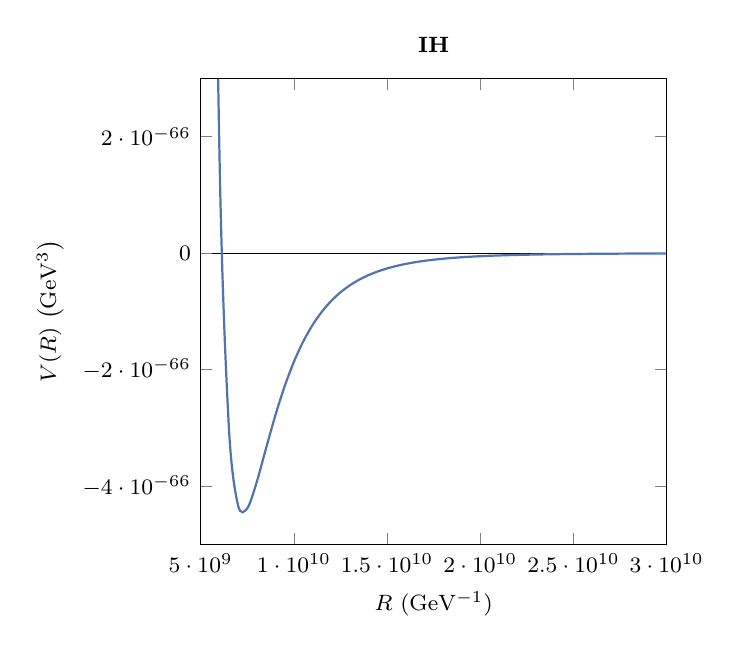
\begin{tikzpicture}
		\begin{axis}	
		[height=7.5cm,
		width=7.5cm, axis on top, ticklabel style = {font=\footnotesize},xmin=5.0e+9,   xmax=3.0e+10,
				ymin=-5.0e-66,   ymax=3.0e-66,title={\footnotesize \textbf{IH}},
		xlabel={\footnotesize $R$ (GeV$^{-1}$)},ylabel={\footnotesize $V(R)$ $\left({\rm GeV}^3\right)$},
		%xtick=\empty,
		%ytick=\empty 
		scaled x ticks=false,
		scaled y ticks=false,
		]
		\addplot[color=black] coordinates {
			(5000000000,0.0)
			(200000000000,0.0)
		};
		\addplot[color=myblue, thick, smooth] coordinates {
        (5000000000,4.777168044571939e-65)
        (5500000000,1.480078836644772e-65)
        (6000000000,1.86838117631501e-66)
        (6500000000,-2.9071272663868833e-66)
        (7000000000,-4.3209963960252063e-66)
        (7500000000,-4.379636900635909e-66)
        (8000000000,-3.9381795787550665e-66)
        (8500000000,-3.359732241481939e-66)
        (9000000000,-2.792574363604154e-66)
        (9500000000,-2.2906256855669978e-66)
        (10000000000,-1.867008016470171e-66)
        (10500000000,-1.5181313629321937e-66)
        (11000000000,-1.2344892576214656e-66)
        (11500000000,-1.005374037529171e-66)
        (12000000000,-8.208000349401838e-67)
        (12500000000,-6.721583948506319e-67)
        (13000000000,-5.5231541916433756e-67)
        (13500000000,-4.5548632606999533e-67)
        (14000000000,-3.7703649390679155e-67)
        (14500000000,-3.1327690177735486e-67)
        (15000000000,-2.6128025419675316e-67)
        (15500000000,-2.1872575656396276e-67)
        (16000000000,-1.8377241481373682e-67)
        (16500000000,-1.549575899874181e-67)
        (17000000000,-1.3111667948997626e-67)
        (17500000000,-1.1131992851641328e-67)
        (18000000000,-9.482288062263602e-68)
        (18500000000,-8.102757133044345e-68)
        (19000000000,-6.945213093511412e-68)
        (19500000000,-5.970694791681632e-68)
        (20000000000,-5.147594381610779e-68)
        (20500000000,-4.4501830496690976e-68)
        (21000000000,-3.857447301417849e-68)
        (21500000000,-3.3521678212898414e-68)
        (22000000000,-2.9201881930778684e-68)
        (22500000000,-2.5498325809048143e-68)
        (23000000000,-2.2314405896047132e-68)
        (23500000000,-1.9569945622262282e-68)
        (24000000000,-1.719820008840215e-68)
        (24500000000,-1.5143440651941773e-68)
        (25000000000,-1.3359001370077279e-68)
        (25500000000,-1.180569414533175e-68)
        (26000000000,-1.0450519099501758e-68)
        (26500000000,-9.265612055166485e-69)
        (27000000000,-8.227383014452564e-69)
        (27500000000,-7.315808945917938e-69)
        (28000000000,-6.5138516012365e-69)
        (28500000000,-5.80697692934204e-69)
        (29000000000,-5.182757280383384e-69)
        (29500000000,-4.630541260801138e-69)
        (30000000000,-4.141179019817175e-69)
        (30500000000,-3.706793076464059e-69)
        (31000000000,-3.320586659458727e-69)
        (31500000000,-2.976683026954322e-69)
        (32000000000,-2.669990435604205e-69)
        (32500000000,-2.3960883982037317e-69)
        (33000000000,-2.1511316534842702e-69)
        (33500000000,-1.9317689075547804e-69)
        (34000000000,-1.7350739234092978e-69)
        (34500000000,-1.5584869561653326e-69)
        (35000000000,-1.3997648758233773e-69)
        (35500000000,-1.2569386011413964e-69)
        (36000000000,-1.1282766995358008e-69)
        (36500000000,-1.0122541982402384e-69)
        (37000000000,-9.075258089010014e-70)
        (37500000000,-8.1290289750625e-70)
        (38000000000,-7.27333638996682e-70)
        (38500000000,-6.498858851035692e-70)
        (39000000000,-5.79732348164455e-70)
        (39500000000,-5.16137765526917e-70)
        (40000000000,-4.584477608261044e-70)
        (40500000000,-4.060791616762111e-70)
        (41000000000,-3.58511569593619e-70)
        (41500000000,-3.152800084546764e-70)
        (42000000000,-2.759685034577468e-70)
        (42500000000,-2.402044642094761e-70)
        (43000000000,-2.076537638512616e-70)
        (43500000000,-1.7801642163138628e-70)
        (44000000000,-1.5102280946497167e-70)
        (44500000000,-1.2643031418468094e-70)
        (45000000000,-1.040203966833977e-70)
        (45500000000,-8.359599724720779e-71)
        (46000000000,-6.49792432910141e-71)
        (46500000000,-4.800942162252218e-71)
        (47000000000,-3.2541182426010343e-71)
        (47500000000,-1.844294650358932e-71)
        (48000000000,-5.595491046483456e-72)
        (48500000000,6.10930757688854e-72)
        (49000000000,1.6769592758914512e-71)
        (49500000000,2.647452466849282e-71)
        (50000000000,3.530516962907528e-71)
        (50500000000,4.333529435443622e-71)
        (51000000000,5.0632075986603296e-71)
        (51500000000,5.725673753413668e-71)
        (52000000000,6.3265117138816494e-71)
        (52500000000,6.870817858041976e-71)
        (53000000000,7.363246954178625e-71)
        (53500000000,7.808053338200647e-71)
        (54000000000,8.20912794890168e-71)
        (54500000000,8.570031669110174e-71)
        (55000000000,8.89402536885111e-71)
        (55500000000,9.18409700119487e-71)
        (56000000000,9.442986061573744e-71)
        (56500000000,9.673205686283854e-71)
        (57000000000,9.877062635039462e-71)
        (57500000000,1.005667537527172e-70)
        (58000000000,1.0213990461900352e-70)
        (58500000000,1.0350797385152632e-70)
        (59000000000,1.0468742040310139e-70)
        (59500000000,1.0569338956726188e-70)
        (60000000000,1.0653982408812877e-70)
        (60500000000,1.0723956518715474e-70)
        (61000000000,1.0780444448873512e-70)
        (61500000000,1.0824536772438048e-70)
        (62000000000,1.0857239100419412e-70)
        (62500000000,1.0879479036346543e-70)
        (63000000000,1.0892112522010542e-70)
        (63500000000,1.0895929631438169e-70)
        (64000000000,1.0891659864506908e-70)
        (64500000000,1.0879976986491119e-70)
        (65000000000,1.086150345525146e-70)
        (65500000000,1.0836814473683128e-70)
        (66000000000,1.0806441701371911e-70)
        (66500000000,1.0770876656119785e-70)
        (67000000000,1.0730573833054515e-70)
        (67500000000,1.0685953566391784e-70)
        (68000000000,1.0637404656541307e-70)
        (68500000000,1.058528678311182e-70)
        (69000000000,1.0529932722446974e-70)
        (69500000000,1.0471650386593308e-70)
        (70000000000,1.0410724699041363e-70)
        (70500000000,1.0347419321174717e-70)
        (71000000000,1.028197824209204e-70)
        (71500000000,1.0214627243321542e-70)
        (72000000000,1.014557524891089e-70)
        (72500000000,1.0075015570439313e-70)
        (73000000000,1.000312705565093e-70)
        (73500000000,9.930075148640705e-71)
        (74000000000,9.856012868829083e-71)
        (74500000000,9.78108171533067e-71)
        (75000000000,9.705412502750174e-71)
        (75500000000,9.629126133919479e-71)
        (76000000000,9.55233431461772e-71)
        (76500000000,9.475140214887355e-71)
        (77000000000,9.397639081169105e-71)
        (77500000000,9.319918803123516e-71)
        (78000000000,9.242060438683591e-71)
        (78500000000,9.164138700588341e-71)
        (79000000000,9.086222407378436e-71)
        (79500000000,9.008374901590256e-71)
        (80000000000,8.930654437660877e-71)
        (80500000000,8.853114541852409e-71)
        (81000000000,8.775804346317463e-71)
        (81500000000,8.69876889925697e-71)
        (82000000000,8.622049452965514e-71)
        (82500000000,8.545683731416605e-71)
        (83000000000,8.469706178909489e-71)
        (83500000000,8.394148191179471e-71)
        (84000000000,8.319038330263764e-71)
        (84500000000,8.244402524314414e-71)
        (85000000000,8.170264253457367e-71)
        (85500000000,8.096644722711996e-71)
        (86000000000,8.023563022907698e-71)
        (86500000000,7.951036280462453e-71)
        (87000000000,7.879079796822664e-71)
        (87500000000,7.807707178303123e-71)
        (88000000000,7.736930457010293e-71)
        (88500000000,7.666760203480954e-71)
        (89000000000,7.597205631621154e-71)
        (89500000000,7.528274696486958e-71)
        (90000000000,7.459974185408504e-71)
        (90500000000,7.392309802922001e-71)
        (91000000000,7.325286249940261e-71)
        (91500000000,7.25890729756103e-71)
        (92000000000,7.193175855883303e-71)
        (92500000000,7.128094038175162e-71)
        (93000000000,7.0636632207119395e-71)
        (93500000000,6.9998840985805815e-71)
        (94000000000,6.936756737725102e-71)
        (94500000000,6.874280623488407e-71)
        (95000000000,6.812454705887688e-71)
        (95500000000,6.751277441843947e-71)
        (96000000000,6.69074683457066e-71)
        (96500000000,6.6308604703122425e-71)
        (97000000000,6.571615552609783e-71)
        (97500000000,6.513008934259076e-71)
        (98000000000,6.455037147114697e-71)
        (98500000000,6.397696429883151e-71)
        (99000000000,6.340982754038434e-71)
        (99500000000,6.284891847984089e-71)
        (100000000000,6.2294192195775385e-71)
        (100500000000,6.174560177124469e-71)
        (101000000000,6.120309848943832e-71)
        (101500000000,6.066663201597218e-71)
        (102000000000,6.013615056870088e-71)
        (102500000000,5.961160107586375e-71)
        (103000000000,5.909292932332717e-71)
        (103500000000,5.858008009163283e-71)
        (104000000000,5.807299728351618e-71)
        (104500000000,5.757162404251452e-71)
        (105000000000,5.707590286324305e-71)
        (105500000000,5.658577569388024e-71)
        (106000000000,5.610118403136714e-71)
        (106500000000,5.562206900979273e-71)
        (107000000000,5.514837148240706e-71)
        (107500000000,5.468003209767404e-71)
        (108000000000,5.421699136975023e-71)
        (108500000000,5.3759189743750156e-71)
        (109000000000,5.330656765613543e-71)
        (109500000000,5.2859065590543815e-71)
        (110000000000,5.24166241293532e-71)
        (110500000000,5.197918400125698e-71)
        (111000000000,5.1546686125110005e-71)
        (111500000000,5.1119071650286405e-71)
        (112000000000,5.069628199377699e-71)
        (112500000000,5.027825887423778e-71)
        (113000000000,4.986494434318876e-71)
        (113500000000,4.945628081354907e-71)
        (114000000000,4.905221108568286e-71)
        (114500000000,4.8652678371119186e-71)
        (115000000000,4.8257626314099045e-71)
        (115500000000,4.786699901109288e-71)
        (116000000000,4.748074102842277e-71)
        (116500000000,4.709879741811533e-71)
        (117000000000,4.6721113732103295e-71)
        (117500000000,4.6347636034886095e-71)
        (118000000000,4.597831091475328e-71)
        (118500000000,4.561308549366778e-71)
        (119000000000,4.52519074359002e-71)
        (119500000000,4.489472495549886e-71)
        (120000000000,4.454148682267662e-71)
        (120500000000,4.419214236918825e-71)
        (121000000000,4.384664149276955e-71)
        (121500000000,4.350493466070346e-71)
        (122000000000,4.3166972912575424e-71)
        (122500000000,4.283270786227527e-71)
        (123000000000,4.2502091699300506e-71)
        (123500000000,4.217507718941126e-71)
        (124000000000,4.185161767468502e-71)
        (124500000000,4.153166707301542e-71)
        (125000000000,4.121517987709725e-71)
        (125500000000,4.0902111152936625e-71)
        (126000000000,4.059241653792324e-71)
        (126500000000,4.028605223849897e-71)
        (127000000000,3.9982975027455284e-71)
        (127500000000,3.968314224088936e-71)
        (128000000000,3.938651177484737e-71)
        (128500000000,3.909304208168139e-71)
        (129000000000,3.880269216614473e-71)
        (129500000000,3.851542158124868e-71)
        (130000000000,3.823119042390267e-71)
        (130500000000,3.794995933035788e-71)
        (131000000000,3.767168947147347e-71)
        (131500000000,3.739634254782312e-71)
        (132000000000,3.7123880784658325e-71)
        (132500000000,3.685426692674428e-71)
        (133000000000,3.6587464233082385e-71)
        (133500000000,3.632343647153338e-71)
        (134000000000,3.606214791335327e-71)
        (134500000000,3.5803563327654178e-71)
        (135000000000,3.5547647975800782e-71)
        (135500000000,3.5294367605752922e-71)
        (136000000000,3.504368844636347e-71)
        (136500000000,3.4795577201640764e-71)
        (137000000000,3.4550001044983487e-71)
        (137500000000,3.4306927613395967e-71)
        (138000000000,3.4066325001690786e-71)
        (138500000000,3.3828161756685407e-71)
        (139000000000,3.359240687139898e-71)
        (139500000000,3.3359029779254946e-71)
        (140000000000,3.312800034829473e-71)
        (140500000000,3.289928887540737e-71)
        (141000000000,3.2672866080579517e-71)
        (141500000000,3.2448703101170103e-71)
        (142000000000,3.2226771486213316e-71)
        (142500000000,3.200704319075339e-71)
        (143000000000,3.1789490570214607e-71)
        (143500000000,3.1574086374809234e-71)
        (144000000000,3.1360803743986186e-71)
        (144500000000,3.114961620092291e-71)
        (145000000000,3.0940497647062586e-71)
        (145500000000,3.0733422356698857e-71)
        (146000000000,3.0528364971609687e-71)
        (146500000000,3.032530049574216e-71)
        (147000000000,3.0124204289949705e-71)
        (147500000000,2.9925052066782855e-71)
        (148000000000,2.9727819885335e-71)
        (148500000000,2.9532484146143846e-71)
        (149000000000,2.9339021586149807e-71)
        (149500000000,2.9147409273711697e-71)
        (150000000000,2.895762460368087e-71)
        (150500000000,2.8769645292533843e-71)
        (151000000000,2.858344937356433e-71)
        (151500000000,2.8399015192134636e-71)
        (152000000000,2.8216321400987008e-71)
        (152500000000,2.8035346955614934e-71)
        (153000000000,2.785607110969464e-71)
        (153500000000,2.7678473410576737e-71)
        (154000000000,2.7502533694838037e-71)
        (154500000000,2.7328232083893525e-71)
        (155000000000,2.7155548979668315e-71)
        (155500000000,2.698446506032936e-71)
        (156000000000,2.6814961276076803e-71)
        (156500000000,2.664701884499462e-71)
        (157000000000,2.648061924896031e-71)
        (157500000000,2.631574422961316e-71)
        (158000000000,2.615237578438094e-71)
        (158500000000,2.5990496162564377e-71)
        (159000000000,2.5830087861479107e-71)
        (159500000000,2.567113362265464e-71)
        (160000000000,2.551361642808978e-71)
        (160500000000,2.535751949656413e-71)
        (161000000000,2.5202826280004907e-71)
        (161500000000,2.5049520459908918e-71)
        (162000000000,2.489758594381867e-71)
        (162500000000,2.474700686185246e-71)
        (163000000000,2.4597767563287587e-71)
        (163500000000,2.444985261319621e-71)
        (164000000000,2.4303246789133275e-71)
        (164500000000,2.415793507787575e-71)
        (165000000000,2.4013902672212757e-71)
        (165500000000,2.387113496778578e-71)
        (166000000000,2.3729617559978476e-71)
        (166500000000,2.3589336240855384e-71)
        (167000000000,2.345027699614887e-71)
        (167500000000,2.331242600229371e-71)
        (168000000000,2.31757696235087e-71)
        (168500000000,2.304029440892461e-71)
        (169000000000,2.290598708975784e-71)
        (169500000000,2.277283457652917e-71)
        (170000000000,2.2640823956326945e-71)
        (170500000000,2.2509942490114096e-71)
        (171000000000,2.238017761007829e-71)
        (171500000000,2.2251516917024685e-71)
        (172000000000,2.212394817781059e-71)
        (172500000000,2.19974593228214e-71)
        (173000000000,2.187203844348727e-71)
        (173500000000,2.1747673789839813e-71)
        (174000000000,2.16243537681083e-71)
        (174500000000,2.15020669383547e-71)
        (175000000000,2.138080201214698e-71)
        (175500000000,2.126054785027013e-71)
        (176000000000,2.1141293460474194e-71)
        (176500000000,2.1023027995258854e-71)
        (177000000000,2.090574074969395e-71)
        (177500000000,2.078942115927533e-71)
        (178000000000,2.067405879781555e-71)
        (178500000000,2.0559643375368733e-71)
        (179000000000,2.0446164736189223e-71)
        (179500000000,2.0333612856723347e-71)
        (180000000000,2.0221977843633744e-71)
        (180500000000,2.0111249931855885e-71)
        (181000000000,2.0001419482686064e-71)
        (181500000000,1.989247698190049e-71)
        (182000000000,1.978441303790494e-71)
        (182500000000,1.9677218379914364e-71)
        (183000000000,1.9570883856162114e-71)
        (183500000000,1.9465400432138254e-71)
        (184000000000,1.936075918885632e-71)
        (184500000000,1.92569513211483e-71)
        (185000000000,1.915396813598723e-71)
        (185500000000,1.9051801050836918e-71)
        (186000000000,1.895044159202842e-71)
        (186500000000,1.884988139316277e-71)
        (187000000000,1.8750112193539605e-71)
        (187500000000,1.8651125836611084e-71)
        (188000000000,1.8552914268460892e-71)
        (188500000000,1.8455469536307725e-71)
        (189000000000,1.8358783787032914e-71)
        (189500000000,1.8262849265731856e-71)
        (190000000000,1.8167658314288686e-71)
        (190500000000,1.8073203369973937e-71)
        (191000000000,1.797947696406474e-71)
        (191500000000,1.7886471720487208e-71)
        (192000000000,1.7794180354480565e-71)
        (192500000000,1.770259567128277e-71)
        (193000000000,1.761171056483713e-71)
        (193500000000,1.7521518016519676e-71)
        (194000000000,1.7432011093886843e-71)
        (194500000000,1.7343182949443185e-71)
        (195000000000,1.7255026819428738e-71)
        (195500000000,1.7167536022625744e-71)
        (196000000000,1.7080703959184346e-71)
        (196500000000,1.699452410946696e-71)
        (197000000000,1.690899003291105e-71)
        (197500000000,1.6824095366909921e-71)
        (198000000000,1.6739833825711254e-71)
        (198500000000,1.665619919933309e-71)
        (199000000000,1.6573185352496985e-71)
        (199500000000,1.6490786223577949e-71)
        (200000000000,1.6408995823571054e-71)
		};
		\end{axis}%
		\end{tikzpicture}%
		\caption{\footnotesize Effective potential for Majorana neutrinos when considering normal hierarchy (left) and inverted hierarchy (right). In both cases the lightest neutrinos is considered massless, $m_{\nu_1}=0$ eV for NH and $m_{\nu_3}=0$ for IH.}
		\label{fig:neutrinosmajorana}
	\end{center}
\end{figure}

\begin{tcolorbox}[width=\textwidth,colback={white},title={\textbf{Note!}},colbacktitle=myblue,coltitle=white]    
From now on the neutrino mass eigenstates will follow the next mass hierarchy according to the one of the PDG~\cite{Olive:2016xmw} (see also Fig.~\ref{fig:normalinverted}.) \par
{\color{myblue}$\bullet$} NH: $m_{\nu_1}< m_{\nu_2} \ll m_{\nu_3}$. \par 
{\color{myblue}$\bullet$} IH: $m_{\nu_3}\ll m_{\nu_1} < m_{\nu_2}$. \par 
\end{tcolorbox} 

\subsection{Majorana neutrinos}

In Fig.~\ref{fig:neutrinosmajorana} the effective potential for Majorana neutrinos is shown where the lightest neutrino has a zero mass. On the left panel of Fig.~\ref{fig:neutrinosmajorana} it is assumed a NH for the neutrinos masses where on the right panel of Fig.~\ref{fig:neutrinosmajorana} it is assumed an IH. An AdS vacuum is formed for this configuration in both hierarchies, that in principle is forbidden by WGC arguments \cite{Ooguri:2016pdq}. If the mass of the lightest neutrino is different from zero, the mass terms of the potential make the potential deeper, this makes the situation with Majorana neutrinos disfavoured. 

\begin{table}
\begin{center}
\begin{tabular}{c | c | c |}
 & NH & IH \\
 \hline
No vacuum & $m_{\nu_1}< 6.7$ meV & $m_{\nu_1}< 2.1$ meV \\
dS$_3$ vacuum & 6.7 meV $<m_{\nu_1}< 7.7$ meV& 2.1 meV $<m_{\nu_1}<$ 2.56 meV \\
AdS$_3$ vacuum & $m_{\nu_1}> 7.7$ meV & $m_{\nu_1}> 2.56$ meV \\
\hline
\end{tabular}
\caption{Ranges of masses of Dirac neutrinos where different vacua configurations are shown.}
\label{tab:dirac}
\end{center}
\end{table}

\subsection{Dirac neutrinos}

In Fig.~\ref{fig:neutrinosdirac} the case of Dirac neutrinos is presented. On the left panel of Fig.~\ref{fig:neutrinosdirac} the NH is assumed. In this case different lightest neutrino masses have been taken into account: 6.0 meV (black), 6.5 meV (green), 7.0 meV (blue), 7.5 meV (brown) and 8.0 meV (red). In this scenario we find different solutions in the effective potential depending on the neutrino masses. For masses greater than 7.73 meV an AdS vacuum is formed, while for masses between 6.7 meV and 7.73 meV a dS vacuum is achieved. In the case where the lightest neutrino is smaller than 6.7 meV there is no vacuum. On the right panel of Fig.~\ref{fig:neutrinosdirac} the IH is assumed. In this case the different colours correspond to the lightest neutrino mass: $m_{\nu_3}=$1.5 meV (black), 2.0 meV (green), 2.5 meV (blue), 3.0 meV (red). For this mass hierarchy we found that for a mass of the lightest neutrino greater than 2.56 meV an AdS vacuum is formed. A dS vacuum is achieved for masses between 2.56 meV and 2.1 meV, and if the lightest neutrino mass is smaller than $m_{\nu_3}<2.1$ meV no vacua is formed. A summary of the masses for which the different vacua are formed is found in Tab.~\ref{tab:dirac}.

\begin{figure}[t]
	\begin{center}
		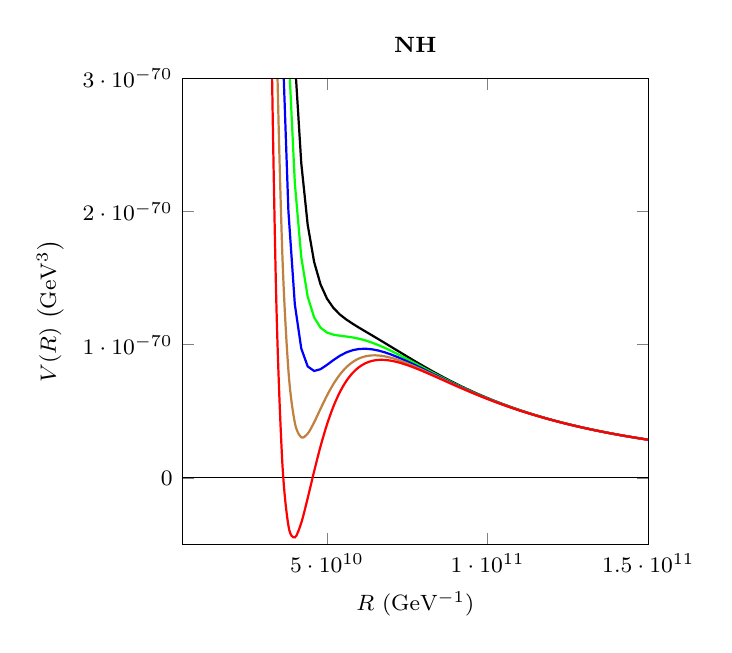
\begin{tikzpicture}
 		\begin{axis}	%[height=8cm,
%		width=8cm,xmin=5.0e+9,   xmax=1.5e+11,
%		ymin=-5.0e-71,   ymax=3.0e-70,title={\textbf{NH}},
%		xlabel=$R$ (GeV$^{-1}$),ylabel=$V(R)$ $\left({\rm GeV}^3\right)$,
%		%xtick=\empty,
%		%ytick=\empty 
%		]
		[height=7.5cm,
		width=7.5cm, axis on top, ticklabel style = {font=\footnotesize},xmin=5.0e+9,   xmax=1.5e+11,
				ymin=-5.0e-71,   ymax=3.0e-70,title={\footnotesize \textbf{NH}},
		xlabel={\footnotesize $R$ (GeV$^{-1}$)},ylabel={\footnotesize $V(R)$ $\left({\rm GeV}^3\right)$},
		%xtick=\empty,
		%ytick=\empty 
		scaled x ticks=false,
		scaled y ticks=false,
		]
		\addplot[color=black] coordinates {
			(2.0e+8,0.0)
			(200000000000,0.0)
		};
		\addplot[color=black, thick] coordinates {
        (26000000000,9.058222462413437e-69)
        (28000000000,5.069184272104761e-69)
        (30000000000,2.918696557571682e-69)
        (32000000000,1.7286694646765925e-69)
        (34000000000,1.0563606597427704e-69)
        (36000000000,6.703460343382939e-70)
        (38000000000,4.459443201560559e-70)
        (40000000000,3.142587164758863e-70)
        (42000000000,2.364069397893355e-70)
        (44000000000,1.9006334814323877e-70)
        (46000000000,1.622316190034791e-70)
        (48000000000,1.4526786490755848e-70)
        (50000000000,1.3464552511817598e-70)
        (52000000000,1.2767591858757458e-70)
        (54000000000,1.227641891016581e-70)
        (56000000000,1.189707602991373e-70)
        (58000000000,1.1574996312452875e-70)
        (60000000000,1.1279286958379604e-70)
        (62000000000,1.0993216770012181e-70)
        (64000000000,1.0708435669929141e-70)
        (66000000000,1.0421458231569374e-70)
        (68000000000,1.0131529661156763e-70)
        (70000000000,9.839339713470473e-71)
        (72000000000,9.546257812670782e-71)
        (74000000000,9.253888358407349e-71)
        (76000000000,8.963821942806446e-71)
        (78000000000,8.677505422786669e-71)
        (80000000000,8.396183032250392e-71)
        (82000000000,8.12087891709823e-71)
        (84000000000,7.852402842190302e-71)
        (86000000000,7.59136793104259e-71)
        (88000000000,7.338213747610058e-71)
        (90000000000,7.0932308045738815e-71)
        (92000000000,6.856584303350134e-71)
        (94000000000,6.628335967086517e-71)
        (96000000000,6.408463465256536e-71)
        (98000000000,6.1968773029837545e-71)
        (100000000000,5.993435258867285e-71)
        (102000000000,5.79795456463318e-71)
        (104000000000,5.610222068200481e-71)
        (106000000000,5.430002633843039e-71)
        (108000000000,5.257046024789695e-71)
        (110000000000,5.0910924945918905e-71)
        (112000000000,4.9318772898392565e-71)
        (114000000000,4.779134241843311e-71)
        (116000000000,4.6325986007349405e-71)
        (118000000000,4.492009243084502e-71)
        (120000000000,4.357110364124731e-71)
        (122000000000,4.227652748062087e-71)
        (124000000000,4.103394694730504e-71)
        (126000000000,3.984102667797152e-71)
        (128000000000,3.869551718649822e-71)
        (130000000000,3.759525730743845e-71)
        (132000000000,3.65381752133287e-71)
        (134000000000,3.552228830939141e-71)
        (136000000000,3.454570225443102e-71)
        (138000000000,3.360660931120252e-71)
        (140000000000,3.2703286191783036e-71)
        (142000000000,3.18340915322417e-71)
        (144000000000,3.0997463105105686e-71)
        (146000000000,3.0191914856857508e-71)
        (148000000000,2.9416033840203115e-71)
        (150000000000,2.866847709648482e-71)
        (152000000000,2.7947968531839312e-71)
        (154000000000,2.7253295821074605e-71)
        (156000000000,2.658330736538689e-71)
        (158000000000,2.5936909323651133e-71)
        (160000000000,2.5313062731840623e-71)
        (162000000000,2.471078072094751e-71)
        (164000000000,2.412912584041287e-71)
        (166000000000,2.356720749138471e-71)
        (168000000000,2.302417947198423e-71)
        (170000000000,2.2499237635076007e-71)
        (172000000000,2.1991617657722485e-71)
        (174000000000,2.1500592920490174e-71)
        (176000000000,2.102547249400785e-71)
        (178000000000,2.056559922960863e-71)
        (180000000000,2.0120347950481405e-71)
        (182000000000,1.968912373947943e-71)
        (184000000000,1.9271360319560693e-71)
        (186000000000,1.886651852274399e-71)
        (188000000000,1.847408484343858e-71)
        (190000000000,1.8093570072031052e-71)
        (192000000000,1.7724508004677265e-71)
        (194000000000,1.736645422534199e-71)
        (196000000000,1.701898495624518e-71)
        (198000000000,1.6681695973006598e-71)
        (200000000000,1.6354201580923775e-71)
		};
		\addplot[color=green, thick] coordinates {
		(26000000000,8.131351196196778e-69)
		(28000000000,4.4355764778746853e-69)
		(30000000000,2.476360306492292e-69)
		(32000000000,1.414159120423993e-69)
		(34000000000,8.291087366712917e-70)
		(36000000000,5.0378304631118864e-70)
		(38000000000,3.222965094043068e-70)
		(40000000000,2.2141061242790554e-70)
		(42000000000,1.659599616811834e-70)
		(44000000000,1.3610668071383315e-70)
		(46000000000,1.2054789096123983e-70)
		(48000000000,1.128102168323189e-70)
		(50000000000,1.0918750667363183e-70)
		(52000000000,1.0757347529613698e-70)
		(54000000000,1.0679156587307879e-70)
		(56000000000,1.062058981915878e-70)
		(58000000000,1.054935041501991e-70)
		(60000000000,1.0451028038692542e-70)
		(62000000000,1.0321195857812518e-70)
		(64000000000,1.0160763175340496e-70)
		(66000000000,9.973264994183965e-71)
		(68000000000,9.763306950343593e-71)
		(70000000000,9.5356988613268e-71)
		(72000000000,9.29499660141964e-71)
		(74000000000,9.045283447470122e-71)
		(76000000000,8.790089117617088e-71)
		(78000000000,8.532385329942478e-71)
		(80000000000,8.274621377221085e-71)
		(82000000000,8.018778223885767e-71)
		(84000000000,7.766428753640882e-71)
		(86000000000,7.51879731545662e-71)
		(88000000000,7.276815025223883e-71)
		(90000000000,7.041169234529097e-71)
		(92000000000,6.812346702955036e-71)
		(94000000000,6.5906706309028835e-71)
		(96000000000,6.3763320269630376e-71)
		(98000000000,6.169416021315157e-71)
		(100000000000,5.969923770776363e-71)
		(102000000000,5.777790578521223e-71)
		(104000000000,5.59290080028413e-71)
		(106000000000,5.41510004567554e-71)
		(108000000000,5.24420511766667e-71)
		(110000000000,5.080012070550465e-71)
		(112000000000,4.922302709370756e-71)
		(114000000000,4.770849802973059e-71)
		(116000000000,4.6254212386214936e-71)
		(118000000000,4.485783308215712e-71)
		(120000000000,4.351703283959475e-71)
		(122000000000,4.22295141421733e-71)
		(124000000000,4.099302447579052e-71)
		(126000000000,3.980536774201513e-71)
		(128000000000,3.866441257742322e-71)
		(130000000000,3.756809818134451e-71)
		(132000000000,3.651443814638512e-71)
		(134000000000,3.550152269675828e-71)
		(136000000000,3.45275196657376e-71)
		(138000000000,3.3590674482787075e-71)
		(140000000000,3.268930939088575e-71)
		(142000000000,3.1821822073395735e-71)
		(144000000000,3.0986683835973956e-71)
		(146000000000,3.01824374612226e-71)
		(148000000000,2.9407694830947898e-71)
		(150000000000,2.86611343921794e-71)
		(152000000000,2.794149852776602e-71)
		(154000000000,2.7247590879816304e-71)
		(156000000000,2.65782736639951e-71)
		(158000000000,2.5932465004321946e-71)
		(160000000000,2.530913631130344e-71)
		(162000000000,2.4707309720696417e-71)
		(164000000000,2.412605560571417e-71)
		(166000000000,2.3564490171866614e-71)
		(168000000000,2.302177314071269e-71)
		(170000000000,2.249710552647218e-71)
		(172000000000,2.1989727507589795e-71)
		(174000000000,2.1498916393879837e-71)
		(176000000000,2.1023984688734342e-71)
		(178000000000,2.056427824499193e-71)
		(180000000000,2.0119174512390853e-71)
		(182000000000,1.9688080874027763e-71)
		(184000000000,1.927043306888043e-71)
		(186000000000,1.886569369720219e-71)
		(188000000000,1.84733508054342e-71)
		(190000000000,1.8092916547192755e-71)
		(192000000000,1.7723925916855552e-71)
		(194000000000,1.7365935552283209e-71)
		(196000000000,1.7018522603258149e-71)
		(198000000000,1.6681283662295843e-71)
		(200000000000,1.6353833754575737e-71)
		};
		\addplot[color=blue, thick] coordinates {
		(26000000000,7.188353960787539e-69)
		(28000000000,3.794155756954165e-69)
		(30000000000,2.0308265863071098e-69)
		(32000000000,1.0989911002826393e-69)
		(34000000000,6.025570010719713e-70)
		(36000000000,3.3860035482733156e-70)
		(38000000000,2.0032100925101637e-70)
		(40000000000,1.303073809535317e-70)
		(42000000000,9.720996150238755e-71)
		(44000000000,8.373689948260115e-71)
		(46000000000,8.031289508365577e-71)
		(48000000000,8.165480677153829e-71)
		(50000000000,8.488796316933866e-71)
		(52000000000,8.84943534387118e-71)
		(54000000000,9.171850024099058e-71)
		(56000000000,9.42291770180509e-71)
		(58000000000,9.592603069292985e-71)
		(60000000000,9.682912831551458e-71)
		(62000000000,9.701631052961212e-71)
		(64000000000,9.658822095777822e-71)
		(66000000000,9.564936235434464e-71)
		(68000000000,9.429839126729495e-71)
		(70000000000,9.262367845403951e-71)
		(72000000000,9.070180730651178e-71)
		(74000000000,8.859765008404014e-71)
		(76000000000,8.636523335056208e-71)
		(78000000000,8.404894231988955e-71)
		(80000000000,8.168481378556409e-71)
		(82000000000,7.930178488732831e-71)
		(84000000000,7.692283334733022e-71)
		(86000000000,7.45659838256857e-71)
		(88000000000,7.224517659372832e-71)
		(90000000000,6.997100596105807e-71)
		(92000000000,6.7751341127395675e-71)
		(94000000000,6.5591843950222005e-71)
		(96000000000,6.349639807055215e-71)
		(98000000000,6.1467462836674816e-71)
		(100000000000,5.950636404140326e-71)
		(102000000000,5.761353194352365e-71)
		(104000000000,5.578869554150727e-71)
		(106000000000,5.403104068808563e-71)
		(108000000000,5.233933841134471e-71)
		(110000000000,5.071204874824395e-71)
		(112000000000,4.91474044923358e-71)
		(114000000000,4.7643478494568685e-71)
		(116000000000,4.619823751743436e-71)
		(118000000000,4.480958511123857e-71)
		(120000000000,4.347539554085055e-71)
		(122000000000,4.219354042747819e-71)
		(124000000000,4.096190947019567e-71)
		(126000000000,3.977842636528747e-71)
		(128000000000,3.8641060838789985e-71)
		(130000000000,3.754783754121644e-71)
		(132000000000,3.649684241692589e-71)
		(134000000000,3.5486227048627276e-71)
		(136000000000,3.4514211385702363e-71)
		(138000000000,3.357908518976867e-71)
		(140000000000,3.2679208469210867e-71)
		(142000000000,3.1813011123845295e-71)
		(144000000000,3.097899197944243e-71)
		(146000000000,3.017571735787674e-71)
		(148000000000,2.940181930085437e-71)
		(150000000000,2.865599354238608e-71)
		(152000000000,2.7936997306520353e-71)
		(154000000000,2.7243646991590788e-71)
		(156000000000,2.657481578975379e-71)
		(158000000000,2.5929431280400736e-71)
		(160000000000,2.5306473027713468e-71)
		(162000000000,2.4704970205858343e-71)
		(164000000000,2.412399926980575e-71)
		(166000000000,2.3562681685294326e-71)
		(168000000000,2.3020181727843476e-71)
		(170000000000,2.2495704357803742e-71)
		(172000000000,2.1988493176094248e-71)
		(174000000000,2.1497828463407302e-71)
		(176000000000,2.1023025304176745e-71)
		(178000000000,2.056343179543823e-71)
		(180000000000,2.0118427339799094e-71)
		(182000000000,1.9687421021034754e-71)
		(184000000000,1.9269850060298415e-71)
		(186000000000,1.8865178350539857e-71)
		(188000000000,1.847289506644906e-71)
		(190000000000,1.8092513347051584e-71)
		(192000000000,1.77235690479651e-71)
		(194000000000,1.7365619560267148e-71)
		(196000000000,1.7018242692909729e-71)
		(198000000000,1.6681035615637871e-71)
		(200000000000,1.6353613859417933e-71)
		};
		\addplot[color=brown, thick, smooth] coordinates {
		(26000000000,6.234767551461487e-69)
		(28000000000,3.1487843874922355e-69)
		(30000000000,1.5848222221755984e-69)
		(32000000000,7.851088916024214e-70)
		(34000000000,3.781005881297016e-70)
		(36000000000,1.7580448567398474e-70)
		(38000000000,8.07460804863937e-71)
		(40000000000,4.147630728544043e-71)
		(42000000000,3.0538045206759905e-71)
		(44000000000,3.3228192355147457e-71)
		(46000000000,4.172229075473805e-71)
		(48000000000,5.193945719063046e-71)
		(50000000000,6.184206387953222e-71)
		(52000000000,7.050227510697154e-71)
		(54000000000,7.758557659294462e-71)
		(56000000000,8.306422817627659e-71)
		(58000000000,8.705883710729119e-71)
		(60000000000,8.975182176934457e-71)
		(62000000000,9.134132788037678e-71)
		(64000000000,9.201785512943354e-71)
		(66000000000,9.195351768797863e-71)
		(68000000000,9.129819892465528e-71)
		(70000000000,9.01793351589543e-71)
		(72000000000,8.870348355298145e-71)
		(74000000000,8.695864688405722e-71)
		(76000000000,8.50167984396779e-71)
		(78000000000,8.293631967972145e-71)
		(80000000000,8.076421585760327e-71)
		(82000000000,7.85380594199963e-71)
		(84000000000,7.6287656295014e-71)
		(86000000000,7.403645287763995e-71)
		(88000000000,7.180271144773733e-71)
		(90000000000,6.960048465401486e-71)
		(92000000000,6.744041890534227e-71)
		(94000000000,6.533041394592983e-71)
		(96000000000,6.327616263154464e-71)
		(98000000000,6.128159155604234e-71)
		(100000000000,5.934922000041253e-71)
		(102000000000,5.748045182556349e-71)
		(104000000000,5.5675812448990845e-71)
		(106000000000,5.393514092925891e-71)
		(108000000000,5.225774540181503e-71)
		(110000000000,5.064252862611815e-71)
		(112000000000,4.908808917631436e-71)
		(114000000000,4.759280279660406e-71)
		(116000000000,4.615488761268157e-71)
		(118000000000,4.477245621135328e-71)
		(120000000000,4.3443557045302244e-71)
		(122000000000,4.216620716678694e-71)
		(124000000000,4.093841792436741e-71)
		(126000000000,3.9758214955266805e-71)
		(128000000000,3.862365356014129e-71)
		(130000000000,3.753283034655597e-71)
		(132000000000,3.648389186394478e-71)
		(134000000000,3.547504081941257e-71)
		(136000000000,3.4504540354838864e-71)
		(138000000000,3.357071677682152e-71)
		(140000000000,3.2671961058362258e-71)
		(142000000000,3.1806729371839467e-71)
		(144000000000,3.097354286429203e-71)
		(146000000000,3.0170986846364477e-71)
		(148000000000,2.9397709533815913e-71)
		(150000000000,2.865242045395768e-71)
		(152000000000,2.793388860767842e-71)
		(154000000000,2.7240940459966444e-71)
		(156000000000,2.6572457817329086e-71)
		(158000000000,2.5927375638653795e-71)
		(160000000000,2.530467981637686e-71)
		(162000000000,2.470340495693134e-71)
		(164000000000,2.412263218301534e-71)
		(166000000000,2.3561486974993164e-71)
		(168000000000,2.301913706449776e-71)
		(170000000000,2.2494790389868575e-71)
		(172000000000,2.1987693120287364e-71)
		(174000000000,2.149712775324698e-71)
		(176000000000,2.102241128820677e-71)
		(178000000000,2.0562893477871557e-71)
		(180000000000,2.0117955157413463e-71)
		(182000000000,1.968700665108188e-71)
		(184000000000,1.926948625497204e-71)
		(186000000000,1.886485879420993e-71)
		(188000000000,1.8472614252429616e-71)
		(190000000000,1.8092266471144272e-71)
		(192000000000,1.7723351916422834e-71)
		(194000000000,1.736542851016394e-71)
		(196000000000,1.7018074523193263e-71)
		(198000000000,1.6680887527388399e-71)
		(200000000000,1.6353483404047662e-71)
		};
		\addplot[color=red, thick, smooth] coordinates {
		(26000000000,5.275604868302248e-69)
		(28000000000,2.5029167213048856e-69)
		(30000000000,1.140753783535515e-69)
		(32000000000,4.742027993690469e-70)
		(34000000000,1.5693330013861137e-70)
		(36000000000,1.6241075611621992e-71)
		(38000000000,-3.5829109077585584e-71)
		(40000000000,-4.4659246994029495e-71)
		(42000000000,-3.3758561613139637e-71)
		(44000000000,-1.5213088433074427e-71)
		(46000000000,4.916803826383675e-72)
		(48000000000,2.3757472829342937e-71)
		(50000000000,4.0108897238070746e-71)
		(52000000000,5.3631734947564154e-71)
		(54000000000,6.4409732140014645e-71)
		(56000000000,7.271558820318886e-71)
		(58000000000,7.8887842067599e-71)
		(60000000000,8.326843514686004e-71)
		(62000000000,8.617327006809675e-71)
		(64000000000,8.788045748227443e-71)
		(66000000000,8.862777348385642e-71)
		(68000000000,8.861465189972015e-71)
		(70000000000,8.800616263256901e-71)
		(72000000000,8.693761887431045e-71)
		(74000000000,8.551912146278898e-71)
		(76000000000,8.383971672253772e-71)
		(78000000000,8.197104386687823e-71)
		(80000000000,7.997045273574761e-71)
		(82000000000,7.788362410103056e-71)
		(84000000000,7.574674686523739e-71)
		(86000000000,7.358831282259252e-71)
		(88000000000,7.143058795524559e-71)
		(90000000000,6.929081381426169e-71)
		(92000000000,6.718218574372217e-71)
		(94000000000,6.511464778694144e-71)
		(96000000000,6.3095537673724224e-71)
		(98000000000,6.113010958214842e-71)
		(100000000000,5.9221957463432384e-71)
		(102000000000,5.737335758321145e-71)
		(104000000000,5.558554549185765e-71)
		(106000000000,5.3858939799591825e-71)
		(108000000000,5.219332280788226e-71)
		(110000000000,5.058798615276119e-71)
		(112000000000,4.904184807394182e-71)
		(114000000000,4.755354767237947e-71)
		(116000000000,4.612152050473159e-71)
		(118000000000,4.474405904170507e-71)
		(120000000000,4.341936085209311e-71)
		(122000000000,4.214556683564145e-71)
		(124000000000,4.092079139155257e-71)
		(126000000000,3.974314605582999e-71)
		(128000000000,3.8610757853925995e-71)
		(130000000000,3.752178338248027e-71)
		(132000000000,3.647441944498805e-71)
		(134000000000,3.546691091267788e-71)
		(136000000000,3.44975563569829e-71)
		(138000000000,3.356471189832794e-71)
		(140000000000,3.2666793633142346e-71)
		(142000000000,3.180227893350444e-71)
		(144000000000,3.096970685876172e-71)
		(146000000000,3.016767787353423e-71)
		(148000000000,2.9394853029815787e-71)
		(150000000000,2.8649952740918154e-71)
		(152000000000,2.7931755250516463e-71)
		(154000000000,2.7239094880047094e-71)
		(156000000000,2.657086012136187e-71)
		(158000000000,2.5925991628189315e-71)
		(160000000000,2.5303480149050775e-71)
		(162000000000,2.4702364435382985e-71)
		(164000000000,2.412172915136671e-71)
		(166000000000,2.3560702806057087e-71)
		(168000000000,2.3018455723611833e-71)
		(170000000000,2.2494198063520817e-71)
		(172000000000,2.1987177899590745e-71)
		(174000000000,2.14966793638981e-71)
		(176000000000,2.102202085988291e-71)
		(178000000000,2.056255334712387e-71)
		(180000000000,2.011765869903902e-71)
		(182000000000,1.968674813373321e-71)
		(184000000000,1.926926071741487e-71)
		(186000000000,1.886466193918809e-71)
		(188000000000,1.8472442355558078e-71)
		(190000000000,1.809211630264063e-71)
		(192000000000,1.7723220673816379e-71)
		(194000000000,1.736531376039924e-71)
		(196000000000,1.7017974152780244e-71)
		(198000000000,1.6680799699450044e-71)
		(200000000000,1.6353406521285127e-71)
		};
		\end{axis}%
		\end{tikzpicture}%
		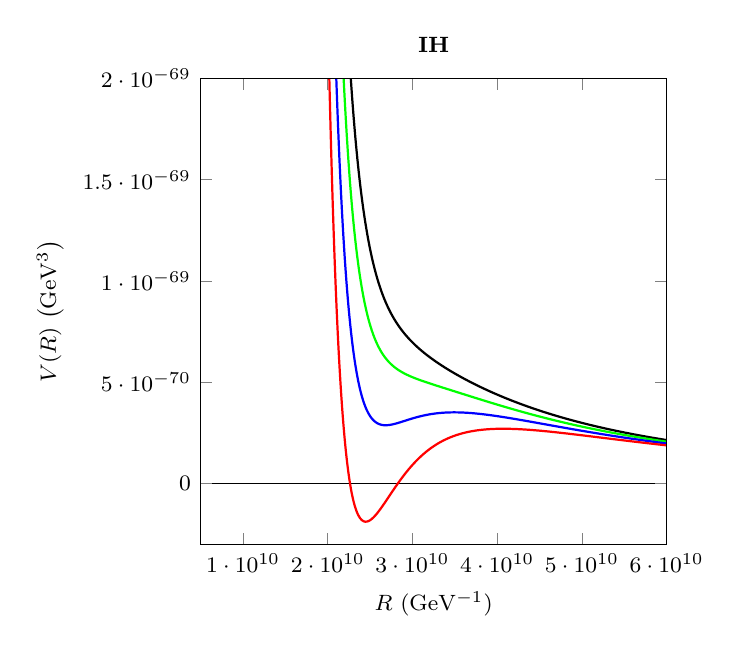
\begin{tikzpicture}
		\begin{axis}	
%		[height=8cm,
%		width=8cm,xmin=5.0e+9,   xmax=6.0e+10,
%		ymin=-3.0e-70,   ymax=2.0e-69,title={\textbf{IH}},
%		xlabel=$R$ (GeV$^{-1}$),ylabel=$V(R)$ $\left({\rm GeV}^3\right)$,
%		%xtick=\empty,
%		%ytick=\empty 
%		]
        [height=7.5cm,
		width=7.5cm, axis on top, ticklabel style = {font=\footnotesize},xmin=5.0e+9,   xmax=6.0e+10,
				ymin=-3.0e-70,   ymax=2.0e-69,title={\footnotesize \textbf{IH}},
		xlabel={\footnotesize $R$ (GeV$^{-1}$)},ylabel={\footnotesize $V(R)$ $\left({\rm GeV}^3\right)$},
		%xtick=\empty,
		%ytick=\empty 
		scaled x ticks=false,
		scaled y ticks=false,
		]
		\addplot[color=black] coordinates {
			(5000000000,0.0)
			(200000000000,0.0)
		};
		\addplot[color=black, thick, smooth] coordinates {
        (19000000000,9.588761587704156e-69)
        (19200000000,8.657919179806009e-69)
        (19400000000,7.830200400783192e-69)
        (19600000000,7.093675279970771e-69)
        (19800000000,6.437847745159812e-69)
        (20000000000,5.85347626891997e-69)
        (20200000000,5.332417894053846e-69)
        (20400000000,4.867492459983326e-69)
        (20600000000,4.452364302506136e-69)
        (20800000000,4.0814390833714285e-69)
        (21000000000,3.749773733778447e-69)
        (21200000000,3.4529977758104946e-69)
        (21400000000,3.187244525231913e-69)
        (21600000000,2.9490908840935723e-69)
        (21800000000,2.7355046073618134e-69)
        (22000000000,2.543798078651669e-69)
        (22200000000,2.371587759770945e-69)
        (22400000000,2.216758590294308e-69)
        (22600000000,2.0774327094036687e-69)
        (22800000000,1.9519419550017183e-69)
        (23000000000,1.8388036665292773e-69)
        (23200000000,1.7366993796054425e-69)
        (23400000000,1.6444560539507102e-69)
        (23600000000,1.5610295222115402e-69)
        (23800000000,1.4854898872952158e-69)
        (24000000000,1.4170086304920828e-69)
        (24200000000,1.3548472227528167e-69)
        (24400000000,1.2983470576250507e-69)
        (24600000000,1.2469205470727133e-69)
        (24800000000,1.2000432411754475e-69)
        (25000000000,1.1572468499201601e-69)
        (25200000000,1.1181130603028204e-69)
        (25400000000,1.0822680550498158e-69)
        (25600000000,1.0493776506915502e-69)
        (25800000000,1.0191429827055664e-69)
        (26000000000,9.912966741735233e-70)
        (26200000000,9.655994320322396e-70)
        (26400000000,9.418370216868022e-70)
        (26600000000,9.198175766113181e-70)
        (26800000000,8.993692047014434e-70)
        (27000000000,8.803378576503804e-70)
        (27200000000,8.625854335782927e-70)
        (27400000000,8.459880866240256e-70)
        (27600000000,8.304347202642347e-70)
        (27800000000,8.158256438181255e-70)
        (28000000000,8.020713739622991e-70)
        (28200000000,7.890915651681703e-70)
        (28400000000,7.768140548133791e-70)
        (28600000000,7.651740103405959e-70)
        (28800000000,7.541131672692573e-70)
        (29000000000,7.435791481294325e-70)
        (29200000000,7.335248535044613e-70)
        (29400000000,7.23907917356089e-70)
        (29600000000,7.146902196794932e-70)
        (29800000000,7.058374503085274e-70)
        (30000000000,6.973187183757833e-70)
        (30200000000,6.89106202538824e-70)
        (30400000000,6.811748376209902e-70)
        (30600000000,6.735020337924374e-70)
        (30800000000,6.660674248394364e-70)
        (31000000000,6.588526424459325e-70)
        (31200000000,6.518411137445014e-70)
        (31400000000,6.450178796904196e-70)
        (31600000000,6.383694320758226e-70)
        (31800000000,6.318835672352257e-70)
        (32000000000,6.255492547023846e-70)
        (32200000000,6.193565192636035e-70)
        (32400000000,6.132963350183862e-70)
        (32600000000,6.073605302051746e-70)
        (32800000000,6.015417016813396e-70)
        (33000000000,5.95833138063699e-70)
        (33200000000,5.902287506399048e-70)
        (33400000000,5.847230112547007e-70)
        (33600000000,5.7931089645772775e-70)
        (33800000000,5.7398783727417006e-70)
        (34000000000,5.687496740258044e-70)
        (34200000000,5.635926156891829e-70)
        (34400000000,5.585132033310313e-70)
        (34600000000,5.535082772079752e-70)
        (34800000000,5.485749471605044e-70)
        (35000000000,5.437105659687939e-70)
        (35200000000,5.389127053722399e-70)
        (35400000000,5.341791344847536e-70)
        (35600000000,5.2950780036541384e-70)
        (35800000000,5.248968105283479e-70)
        (36000000000,5.2034441719765704e-70)
        (36200000000,5.158490031329533e-70)
        (36400000000,5.1140906886856255e-70)
        (36600000000,5.070232212253858e-70)
        (36800000000,5.026901629685612e-70)
        (37000000000,4.9840868349678534e-70)
        (37200000000,4.941776504606235e-70)
        (37400000000,4.899960022174678e-70)
        (37600000000,4.858627410399598e-70)
        (37800000000,4.817769270029748e-70)
        (38000000000,4.7773767248189854e-70)
        (38200000000,4.737441372013722e-70)
        (38400000000,4.6979552377997336e-70)
        (38600000000,4.658910737215147e-70)
        (38800000000,4.620300638086827e-70)
        (39000000000,4.582118028590264e-70)
        (39200000000,4.544356288073172e-70)
        (39400000000,4.507009060818377e-70)
        (39600000000,4.4700702324537944e-70)
        (39800000000,4.433533908745674e-70)
        (40000000000,4.397394396538381e-70)
        (40200000000,4.361646186625711e-70)
        (40400000000,4.326283938361778e-70)
        (40600000000,4.291302465836892e-70)
        (40800000000,4.256696725461981e-70)
        (41000000000,4.2224618048201225e-70)
        (41200000000,4.188592912657842e-70)
        (41400000000,4.155085369901371e-70)
        (41600000000,4.1219346015942945e-70)
        (41800000000,4.089136129663329e-70)
        (42000000000,4.0566855664281585e-70)
        (42200000000,4.024578608779512e-70)
        (42400000000,3.992811032957276e-70)
        (42600000000,3.9613786898670284e-70)
        (42800000000,3.9302775008796234e-70)
        (43000000000,3.8995034540639176e-70)
        (43200000000,3.869052600807562e-70)
        (43400000000,3.8389210527855955e-70)
        (43600000000,3.809104979240125e-70)
        (43800000000,3.779600604538583e-70)
        (44000000000,3.750404205980726e-70)
        (44200000000,3.7215121118281767e-70)
        (44400000000,3.6929206995323565e-70)
        (44600000000,3.664626394139536e-70)
        (44800000000,3.636625666853576e-70)
        (45000000000,3.608915033739297e-70)
        (45200000000,3.581491054550533e-70)
        (45400000000,3.5543503316693815e-70)
        (45600000000,3.5274895091438017e-70)
        (45800000000,3.500905271812486e-70)
        (46000000000,3.474594344506972e-70)
        (46200000000,3.448553491322023e-70)
        (46400000000,3.4227795149461446e-70)
        (46600000000,3.3972692560451535e-70)
        (46800000000,3.372019592692385e-70)
        (47000000000,3.3470274398397345e-70)
        (47200000000,3.3222897488245144e-70)
        (47400000000,3.2978035069076184e-70)
        (47600000000,3.273565736838847e-70)
        (47800000000,3.2495734964458984e-70)
        (48000000000,3.225823878243878e-70)
        (48200000000,3.202314009062438e-70)
        (48400000000,3.1790410496881366e-70)
        (48600000000,3.156002194519805e-70)
        (48800000000,3.133194671234971e-70)
        (49000000000,3.110615740465724e-70)
        (49200000000,3.088262695482505e-70)
        (49400000000,3.066132861884497e-70)
        (49600000000,3.044223597295585e-70)
        (49800000000,3.022532291064843e-70)
        (50000000000,3.0010563639707416e-70)
        (50200000000,2.9797932679283685e-70)
        (50400000000,2.958740485699026e-70)
        (50600000000,2.937895530601726e-70)
        (50800000000,2.917255946226137e-70)
        (51000000000,2.896819306146587e-70)
        (51200000000,2.8765832136368643e-70)
        (51400000000,2.8565453013856232e-70)
        (51600000000,2.836703231212076e-70)
        (51800000000,2.8170546937819893e-70)
        (52000000000,2.7975974083237564e-70)
        (52200000000,2.778329122344544e-70)
        (52400000000,2.7592476113464206e-70)
        (52600000000,2.7403506785424982e-70)
        (52800000000,2.721636154573091e-70)
        (53000000000,2.7031018972218247e-70)
        (53200000000,2.68474579113189e-70)
        (53400000000,2.6665657475223285e-70)
        (53600000000,2.6485597039045502e-70)
        (53800000000,2.6307256237990323e-70)
        (54000000000,2.6130614964523805e-70)
        (54200000000,2.595565336554783e-70)
        (54400000000,2.5782351839579226e-70)
        (54600000000,2.561069103393508e-70)
        (54800000000,2.5440651841924443e-70)
        (55000000000,2.5272215400047725e-70)
        (55200000000,2.510536308520469e-70)
        (55400000000,2.4940076511911927e-70)
        (55600000000,2.4776337529530617e-70)
        (55800000000,2.4614128219505744e-70)
        (56000000000,2.4453430892617273e-70)
        (56200000000,2.4294228086244646e-70)
        (56400000000,2.4136502561644755e-70)
        (56600000000,2.3980237301245058e-70)
        (56800000000,2.382541550595162e-70)
        (57000000000,2.367202059247385e-70)
        (57200000000,2.352003619066569e-70)
        (57400000000,2.3369446140884735e-70)
        (57600000000,2.3220234491369283e-70)
        (57800000000,2.3072385495634444e-70)
        (58000000000,2.2925883609887462e-70)
        (58200000000,2.278071349046309e-70)
        (58400000000,2.263685999127938e-70)
        (58600000000,2.2494308161314334e-70)
        (58800000000,2.2353043242104053e-70)
        (59000000000,2.2213050665262454e-70)
        (59200000000,2.2074316050023293e-70)
        (59400000000,2.193682520080456e-70)
        (59600000000,2.1800564104795745e-70)
        (59800000000,2.1665518929568142e-70)
        (60000000000,2.1531676020708458e-70)
		};
		\addplot[color=green, thick, smooth] coordinates {
		(18800000000,9.379612140086792e-69)
		(19000000000,8.38736937189592e-69)
		(19200000000,7.50883416352772e-69)
		(19400000000,6.730627797857002e-69)
		(19600000000,6.040997671363424e-69)
		(19800000000,5.4296120503313e-69)
		(20000000000,4.887381801777342e-69)
		(20200000000,4.4063054029294915e-69)
		(20400000000,3.97933406130661e-69)
		(20600000000,3.600254226949875e-69)
		(20800000000,3.2635851613624016e-69)
		(21000000000,2.964489554501254e-69)
		(21200000000,2.698695460281886e-69)
		(21400000000,2.4624280597918126e-69)
		(21600000000,2.2523499658177566e-69)
		(21800000000,2.0655089575198173e-69)
		(22000000000,1.8992921844709842e-69)
		(22200000000,1.7513860084868962e-69)
		(22400000000,1.6197407627985683e-69)
		(22600000000,1.5025398038067648e-69)
		(22800000000,1.3981723131237415e-69)
		(23000000000,1.30520937876602e-69)
		(23200000000,1.2223829458114248e-69)
		(23400000000,1.1485672799592731e-69)
		(23600000000,1.0827626334028172e-69)
		(23800000000,1.0240808422389435e-69)
		(24000000000,9.717326191572268e-70)
		(24200000000,9.250163351022954e-70)
		(24400000000,8.83308109615783e-70)
		(24600000000,8.46053052173783e-70)
		(24800000000,8.127575165071336e-70)
		(25000000000,7.829822470177703e-70)
		(25200000000,7.563363113299088e-70)
		(25400000000,7.324717260301566e-70)
		(25600000000,7.110786940099645e-70)
		(25800000000,6.918813817478549e-70)
		(26000000000,6.74634173540978e-70)
		(26200000000,6.591183472837212e-70)
		(26400000000,6.451391230327383e-70)
		(26600000000,6.32523041417006e-70)
		(26800000000,6.211156340516705e-70)
		(27000000000,6.107793525895886e-70)
		(27200000000,6.013917269730926e-70)
		(27400000000,5.928437268980441e-70)
		(27600000000,5.850383035364504e-70)
		(27800000000,5.77889091230932e-70)
		(28000000000,5.7131925122219574e-70)
		(28200000000,5.6526044153898166e-70)
		(28400000000,5.596518990010503e-70)
		(28600000000,5.544396208930198e-70)
		(28800000000,5.495756352834896e-70)
		(29000000000,5.450173502150987e-70)
		(29200000000,5.407269730961514e-70)
		(29400000000,5.366709926005763e-70)
		(29600000000,5.328197162464138e-70)
		(29800000000,5.291468575865764e-70)
		(30000000000,5.256291676217906e-70)
		(30200000000,5.222461056437001e-70)
		(30400000000,5.189795452470864e-70)
		(30600000000,5.1581351171946284e-70)
		(30800000000,5.127339474338765e-70)
		(31000000000,5.097285022399635e-70)
		(31200000000,5.0678634617732356e-70)
		(31400000000,5.038980021260749e-70)
		(31600000000,5.0105519626909704e-70)
		(31800000000,4.982507244704273e-70)
		(32000000000,4.9547833287902576e-70)
		(32200000000,4.927326112492843e-70)
		(32400000000,4.900088976317467e-70)
		(32600000000,4.8730319323176536e-70)
		(32800000000,4.846120863623295e-70)
		(33000000000,4.819326845318784e-70)
		(33200000000,4.792625538098556e-70)
		(33400000000,4.7659966470382417e-70)
		(33600000000,4.739423438631185e-70)
		(33800000000,4.712892309964679e-70)
		(34000000000,4.686392404555045e-70)
		(34200000000,4.659915269939702e-70)
		(34400000000,4.6334545526387286e-70)
		(34600000000,4.6070057265586486e-70)
		(34800000000,4.580565851323213e-70)
		(35000000000,4.5541333573841155e-70)
		(35200000000,4.527707855091842e-70)
		(35400000000,4.501289965203158e-70)
		(35600000000,4.474881168563237e-70)
		(35800000000,4.448483672936751e-70)
		(36000000000,4.4221002951733905e-70)
		(36200000000,4.395734357080262e-70)
		(36400000000,4.369389593545353e-70)
		(36600000000,4.343070071604818e-70)
		(36800000000,4.3167801192845925e-70)
		(37000000000,4.290524263167243e-70)
		(37200000000,4.2643071737439866e-70)
		(37400000000,4.238133617709878e-70)
		(37600000000,4.212008416447221e-70)
		(37800000000,4.1859364100207934e-70)
		(38000000000,4.159922426079083e-70)
		(38200000000,4.1339712531187675e-70)
		(38400000000,4.108087617625853e-70)
		(38600000000,4.082276164658371e-70)
		(38800000000,4.0565414414804794e-70)
		(39000000000,4.030887883899106e-70)
		(39200000000,4.0053198049906684e-70)
		(39400000000,3.9798413859382884e-70)
		(39600000000,3.954456668729886e-70)
		(39800000000,3.9291695504933283e-70)
		(40000000000,3.903983779269338e-70)
		(40200000000,3.8789029510432825e-70)
		(40400000000,3.853930507877351e-70)
		(40600000000,3.8290697370003635e-70)
		(40800000000,3.804323770729026e-70)
		(41000000000,3.7796955871076654e-70)
		(41200000000,3.7551880111659347e-70)
		(41400000000,3.730803716705239e-70)
		(41600000000,3.706545228534529e-70)
		(41800000000,3.6824149250849495e-70)
		(42000000000,3.658415041340997e-70)
		(42200000000,3.634547672032686e-70)
		(42400000000,3.610814775040156e-70)
		(42600000000,3.5872181749674744e-70)
		(42800000000,3.563759566847579e-70)
		(43000000000,3.5404405199450425e-70)
		(43200000000,3.517262481627574e-70)
		(43400000000,3.494226781280255e-70)
		(43600000000,3.471334634240682e-70)
		(43800000000,3.4485871457352824e-70)
		(44000000000,3.425985314800124e-70)
		(44200000000,3.403530038171897e-70)
		(44400000000,3.381222114136508e-70)
		(44600000000,3.3590622463248627e-70)
		(44800000000,3.337051047446911e-70)
		(45000000000,3.315189042956498e-70)
		(45200000000,3.293476674640865e-70)
		(45400000000,3.2719143041297854e-70)
		(45600000000,3.250502216320289e-70)
		(45800000000,3.229240622713884e-70)
		(46000000000,3.208129664663848e-70)
		(46200000000,3.1871694165310406e-70)
		(46400000000,3.166359888746978e-70)
		(46600000000,3.145701030783884e-70)
		(46800000000,3.125192734031311e-70)
		(47000000000,3.104834834579939e-70)
		(47200000000,3.084627115912911e-70)
		(47400000000,3.064569311505909e-70)
		(47600000000,3.04466110733689e-70)
		(47800000000,3.0249021443070825e-70)
		(48000000000,3.005292020574696e-70)
		(48200000000,2.985830293803085e-70)
		(48400000000,2.966516483325215e-70)
		(48600000000,2.947350072226356e-70)
		(48800000000,2.9283305093470063e-70)
		(49000000000,2.909457211208105e-70)
		(49200000000,2.8907295638606647e-70)
		(49400000000,2.872146924661941e-70)
		(49600000000,2.8537086239802748e-70)
		(49800000000,2.83541396683078e-70)
		(50000000000,2.8172622344440565e-70)
		(50200000000,2.7992526857699567e-70)
		(50400000000,2.7813845589186593e-70)
		(50600000000,2.763657072541042e-70)
		(50800000000,2.746069427150454e-70)
		(51000000000,2.7286208063878898e-70)
		(51200000000,2.7113103782325948e-70)
		(51400000000,2.6941372961599726e-70)
		(51600000000,2.6771007002487705e-70)
		(51800000000,2.660199718239345e-70)
		(52000000000,2.6434334665448693e-70)
		(52200000000,2.6268010512171634e-70)
		(52400000000,2.6103015688689342e-70)
		(52600000000,2.5939341075540544e-70)
		(52800000000,2.5776977476075044e-70)
		(53000000000,2.5615915624465133e-70)
		(53200000000,2.5456146193344606e-70)
		(53400000000,2.529765980108949e-70)
		(53600000000,2.5140447018755394e-70)
		(53800000000,2.4984498376684453e-70)
		(54000000000,2.4829804370795344e-70)
		(54200000000,2.4676355468569762e-70)
		(54400000000,2.452414211474656e-70)
		(54600000000,2.4373154736736505e-70)
		(54800000000,2.4223383749768674e-70)
		(55000000000,2.407481956177924e-70)
		(55200000000,2.3927452578054194e-70)
		(55400000000,2.3781273205635295e-70)
		(55600000000,2.3636271857499646e-70)
		(55800000000,2.3492438956522392e-70)
		(56000000000,2.334976493923154e-70)
		(56200000000,2.320824025936379e-70)
		(56400000000,2.306785539122961e-70)
		(56600000000,2.292860083289624e-70)
		(56800000000,2.2790467109195555e-70)
		(57000000000,2.265344477456529e-70)
		(57200000000,2.2517524415730035e-70)
		(57400000000,2.2382696654229324e-70)
		(57600000000,2.2248952148799392e-70)
		(57800000000,2.2116281597614953e-70)
		(58000000000,2.198467574039716e-70)
		(58200000000,2.185412536039355e-70)
		(58400000000,2.1724621286235725e-70)
		(58600000000,2.1596154393680203e-70)
		(58800000000,2.1468715607237387e-70)
		(59000000000,2.1342295901694048e-70)
		(59200000000,2.1216886303533597e-70)
		(59400000000,2.109247789225933e-70)
		(59600000000,2.0969061801624346e-70)
		(59800000000,2.084662922077307e-70)
		(60000000000,2.0725171395297812e-70)
		};
		\addplot[color=blue, thick, smooth] coordinates {
		(18600000000,8.893141862998179e-69)
		(18800000000,7.844307533741259e-69)
		(19000000000,6.920439942406325e-69)
		(19200000000,6.106557470438776e-69)
		(19400000000,5.38952157139583e-69)
		(19600000000,4.757801904606378e-69)
		(19800000000,4.2012726027993054e-69)
		(20000000000,3.711035372495347e-69)
		(20200000000,3.2792657456318554e-69)
		(20400000000,2.8990793274612695e-69)
		(20600000000,2.564415333829214e-69)
		(20800000000,2.269935092682601e-69)
		(21000000000,2.0109335103115873e-69)
		(21200000000,1.7832617809730316e-69)
		(21400000000,1.5832598563982998e-69)
		(21600000000,1.407697395322625e-69)
		(21800000000,1.2537220877225178e-69)
		(22000000000,1.1188143982197925e-69)
		(22200000000,1.000747901783196e-69)
		(22400000000,8.975544955025572e-70)
		(22600000000,8.074938654710806e-70)
		(22800000000,7.290266698987907e-70)
		(23000000000,6.60790970398647e-70)
		(23200000000,6.015815045315739e-70)
		(23400000000,5.503314455548497e-70)
		(23600000000,5.060963410434635e-70)
		(23800000000,4.6803996165451636e-70)
		(24000000000,4.354218256270182e-70)
		(24200000000,4.075861943871328e-70)
		(24400000000,3.8395236048363654e-70)
		(24600000000,3.6400607154806556e-70)
		(24800000000,3.4729195351855056e-70)
		(25000000000,3.3340681337755234e-70)
		(25200000000,3.2199371647687076e-70)
		(25400000000,3.127367464453733e-70)
		(25600000000,3.053563669510842e-70)
		(25800000000,2.9960531443670555e-70)
		(26000000000,2.9526495955147776e-70)
		(26200000000,2.921420825292255e-70)
		(26400000000,2.900660143467267e-70)
		(26600000000,2.8888610126550686e-70)
		(26800000000,2.8846945541380505e-70)
		(27000000000,2.886989584992831e-70)
		(27200000000,2.8947148963239067e-70)
		(27400000000,2.906963516563467e-70)
		(27600000000,2.922938733814042e-70)
		(27800000000,2.941941677596554e-70)
		(28000000000,2.963360283588874e-70)
		(28200000000,2.9866594853714187e-70)
		(28400000000,3.011372495201249e-70)
		(28600000000,3.0370930517030175e-70)
		(28800000000,3.0634685263487537e-70)
		(29000000000,3.0901937929503086e-70)
		(29200000000,3.1170057752764186e-70)
		(29400000000,3.143678597536044e-70)
		(29600000000,3.170019270972088e-70)
		(29800000000,3.195863857328993e-70)
		(30000000000,3.221074056609864e-70)
		(30200000000,3.245534172426038e-70)
		(30400000000,3.2691484134509517e-70)
		(30600000000,3.2918384941128384e-70)
		(30800000000,3.3135415017479764e-70)
		(31000000000,3.334208001065028e-70)
		(31200000000,3.353800349992782e-70)
		(31400000000,3.37229120383342e-70)
		(31600000000,3.389662187183432e-70)
		(31800000000,3.40590271533407e-70)
		(32000000000,3.421008948861337e-70)
		(32200000000,3.43498286689829e-70)
		(32400000000,3.447831446157426e-70)
		(32600000000,3.459565934181302e-70)
		(32800000000,3.470201206547582e-70)
		(33000000000,3.4797551988696786e-70)
		(33200000000,3.48824840542414e-70)
		(33400000000,3.495703437119452e-70)
		(33600000000,3.50214463230705e-70)
		(33800000000,3.5075977146362074e-70)
		(34000000000,3.5120894927785765e-70)
		(34200000000,3.515647597406206e-70)
		(34400000000,3.518300251302319e-70)
		(34600000000,3.520076068928465e-70)
		(34800000000,3.5210038821652924e-70)
		(35000000000,3.521112589299094e-70)
		(35200000000,3.520431024639785e-70)
		(35400000000,3.518987846437185e-70)
		(35600000000,3.516811441014341e-70)
		(35800000000,3.513929841260326e-70)
		(36000000000,3.5103706578253055e-70)
		(36200000000,3.506161021539546e-70)
		(36400000000,3.501327535738282e-70)
		(36600000000,3.495896237316691e-70)
		(36800000000,3.489892565467461e-70)
		(37000000000,3.483341337166863e-70)
		(37200000000,3.4762667285777053e-70)
		(37400000000,3.4686922616289494e-70)
		(37600000000,3.460640795112028e-70)
		(37800000000,3.4521345197082524e-70)
		(38000000000,3.443194956425359e-70)
		(38200000000,3.4338429579807915e-70)
		(38400000000,3.424098712719605e-70)
		(38600000000,3.4139817507030066e-70)
		(38800000000,3.403510951643896e-70)
		(39000000000,3.3927045544029425e-70)
		(39200000000,3.3815801677926565e-70)
		(39400000000,3.37015478246517e-70)
		(39600000000,3.358444783686862e-70)
		(39800000000,3.346465964826128e-70)
		(40000000000,3.3342335414012495e-70)
		(40200000000,3.321762165554781e-70)
		(40400000000,3.309065940836869e-70)
		(40600000000,3.296158437195002e-70)
		(40800000000,3.283052706081243e-70)
		(41000000000,3.269761295599106e-70)
		(41200000000,3.256296265623524e-70)
		(41400000000,3.2426692028358043e-70)
		(41600000000,3.2288912356245886e-70)
		(41800000000,3.2149730488103e-70)
		(42000000000,3.2009248981578113e-70)
		(42200000000,3.1867566246473083e-70)
		(42400000000,3.172477668478757e-70)
		(42600000000,3.1580970827893046e-70)
		(42800000000,3.143623547067818e-70)
		(43000000000,3.129065380253188e-70)
		(43200000000,3.1144305535070255e-70)
		(43400000000,3.0997267026531607e-70)
		(43600000000,3.084961140279592e-70)
		(43800000000,3.070140867499828e-70)
		(44000000000,3.0552725853727284e-70)
		(44200000000,3.0403627059813e-70)
		(44400000000,3.02541736317248e-70)
		(44600000000,3.010442422960647e-70)
		(44800000000,2.9954434935989963e-70)
		(45000000000,2.980425935323389e-70)
		(45200000000,2.965394869774286e-70)
		(45400000000,2.95035518910258e-70)
		(45600000000,2.9353115647659644e-70)
		(45800000000,2.9202684560225835e-70)
		(46000000000,2.9052301181291604e-70)
		(46200000000,2.8902006102509723e-70)
		(46400000000,2.8751838030911432e-70)
		(46600000000,2.8601833862470558e-70)
		(46800000000,2.8452028753013524e-70)
		(47000000000,2.8302456186554905e-70)
		(47200000000,2.8153148041134673e-70)
		(47400000000,2.8004134652233754e-70)
		(47600000000,2.7855444873844702e-70)
		(47800000000,2.7707106137271938e-70)
		(48000000000,2.7559144507736834e-70)
		(48200000000,2.74115847388593e-70)
		(48400000000,2.7264450325088445e-70)
		(48600000000,2.7117763552151934e-70)
		(48800000000,2.6971545545592324e-70)
		(49000000000,2.68258163174581e-70)
		(49200000000,2.6680594811213698e-70)
		(49400000000,2.653589894493257e-70)
		(49600000000,2.639174565283504e-70)
		(49800000000,2.624815092523049e-70)
		(50000000000,2.6105129846922732e-70)
		(50200000000,2.5962696634134643e-70)
		(50400000000,2.582086467000658e-70)
		(50600000000,2.5679646538722375e-70)
		(50800000000,2.5539054058313038e-70)
		(51000000000,2.5399098312188838e-70)
		(51200000000,2.5259789679446893e-70)
		(51400000000,2.5121137864000992e-70)
		(51600000000,2.498315192257782e-70)
		(51800000000,2.484584029162365e-70)
		(52000000000,2.4709210813162037e-70)
		(52200000000,2.457327075964312e-70)
		(52400000000,2.4438026857823645e-70)
		(52600000000,2.4303485311713787e-70)
		(52800000000,2.4169651824628136e-70)
		(53000000000,2.4036531620374133e-70)
		(53200000000,2.390412946361193e-70)
		(53400000000,2.3772449679417953e-70)
		(53600000000,2.3641496172081908e-70)
		(53800000000,2.3511272443168552e-70)
		(54000000000,2.338178160887099e-70)
		(54200000000,2.3253026416684578e-70)
		(54400000000,2.312500926142671e-70)
		(54600000000,2.2997732200628412e-70)
		(54800000000,2.2871196969322195e-70)
		(55000000000,2.274540499424935e-70)
		(55200000000,2.2620357407509602e-70)
		(55400000000,2.2496055059674507e-70)
		(55600000000,2.2372498532385853e-70)
		(55800000000,2.2249688150458622e-70)
		(56000000000,2.2127623993508126e-70)
		(56200000000,2.2006305907119918e-70)
		(56400000000,2.1885733513579725e-70)
		(56600000000,2.176590622218124e-70)
		(56800000000,2.164682323912754e-70)
		(57000000000,2.1528483577042462e-70)
		(57200000000,2.141088606410659e-70)
		(57400000000,2.1294029352832727e-70)
		(57600000000,2.1177911928495024e-70)
		(57800000000,2.1062532117224653e-70)
		(58000000000,2.0947888093785446e-70)
		(58200000000,2.083397788904179e-70)
		(58400000000,2.0720799397130487e-70)
		(58600000000,2.0608350382348354e-70)
		(58800000000,2.049662848576635e-70)
		(59000000000,2.0385631231580914e-70)
		(59200000000,2.0275356033212552e-70)
		(59400000000,2.0165800199161657e-70)
		(59600000000,2.0056960938630654e-70)
		(59800000000,1.994883536692176e-70)
		(60000000000,1.9841420510618824e-70)
		};
		\addplot[color=red, thick, smooth] coordinates {
		(18200000000,9.382041993839239e-69)
		(18400000000,8.125141660355514e-69)
		(18600000000,7.024407310147633e-69)
		(18800000000,6.06067943720214e-69)
		(19000000000,5.217197617331647e-69)
		(19200000000,4.4792898754297024e-69)
		(19400000000,3.834103872438418e-69)
		(19600000000,3.270374044423528e-69)
		(19800000000,2.778219684839771e-69)
		(20000000000,2.3489696886912426e-69)
		(20200000000,1.975010294703692e-69)
		(20400000000,1.6496526862223814e-69)
		(20600000000,1.367017757875038e-69)
		(20800000000,1.1219357352484761e-69)
		(21000000000,9.098586591343402e-70)
		(21200000000,7.267840228465118e-70)
		(21400000000,5.691880879164856e-70)
		(21600000000,4.339676061758819e-70)
		(21800000000,3.18388849953913e-70)
		(22000000000,2.200430011645947e-70)
		(22200000000,1.3680707807051592e-70)
		(22400000000,6.680968858542422e-71)
		(22600000000,8.400993716386566e-72)
		(22800000000,-3.987365361985287e-71)
		(23000000000,-7.92968587652972e-71)
		(23200000000,-1.10999528050737e-70)
		(23400000000,-1.3597875513366157e-70)
		(23600000000,-1.551135565562072e-70)
		(23800000000,-1.6917872279646276e-70)
		(24000000000,-1.7885701699758045e-70)
		(24200000000,-1.84749923992598e-70)
		(24400000000,-1.8738712657530796e-70)
		(24600000000,-1.8723486366896518e-70)
		(24800000000,-1.8470330565113465e-70)
		(25000000000,-1.8015306521976995e-70)
		(25200000000,-1.7390094748634164e-70)
		(25400000000,-1.6622503017135983e-70)
		(25600000000,-1.5736915360066064e-70)
		(25800000000,-1.475468904481075e-70)
		(26000000000,-1.3694505664414557e-70)
		(26200000000,-1.2572681742099971e-70)
		(26400000000,-1.1403443594684745e-70)
		(26600000000,-1.0199170629359597e-70)
		(26800000000,-8.970610748471218e-71)
		(27000000000,-7.727071098690232e-71)
		(27200000000,-6.476587016480236e-71)
		(27400000000,-5.226071684408855e-71)
		(27600000000,-3.981448716434829e-71)
		(27800000000,-2.7477696299085786e-71)
		(28000000000,-1.529317932927084e-71)
		(28200000000,-3.297013542482652e-72)
		(28400000000,8.48066434484177e-72)
		(28600000000,2.001493410692348e-71)
		(28800000000,3.1285450512009313e-71)
		(29000000000,4.227587506613819e-71)
		(29200000000,5.297337272500803e-71)
		(29400000000,6.3368166247651e-71)
		(29600000000,7.345314170043728e-71)
		(29800000000,8.32234993581593e-71)
		(30000000000,9.267644490098328e-71)
		(30200000000,1.0181091638289656e-70)
		(30400000000,1.106273429579034e-70)
		(30600000000,1.1912743180164717e-70)
		(30800000000,1.2731398006627036e-70)
		(31000000000,1.3519070906073866e-70)
		(31200000000,1.4276211816287963e-70)
		(31400000000,1.500333562476364e-70)
		(31600000000,1.570101086631876e-70)
		(31800000000,1.6369849800539478e-70)
		(32000000000,1.701049971357272e-70)
		(32200000000,1.762363530600995e-70)
		(32400000000,1.820995204395762e-70)
		(32600000000,1.8770160363996105e-70)
		(32800000000,1.9304980634824776e-70)
		(33000000000,1.9815138789156947e-70)
		(33200000000,2.0301362548974296e-70)
		(33400000000,2.076437817576011e-70)
		(33600000000,2.1204907684905697e-70)
		(33800000000,2.1623666470185445e-70)
		(34000000000,2.2021361290218127e-70)
		(34200000000,2.239868857412412e-70)
		(34400000000,2.2756333008371678e-70)
		(34600000000,2.3094966370993598e-70)
		(34800000000,2.341524658314542e-70)
		(35000000000,2.371781695129877e-70)
		(35200000000,2.4003305576377426e-70)
		(35400000000,2.4272324908771448e-70)
		(35600000000,2.4525471430548232e-70)
		(35800000000,2.476332544828586e-70)
		(36000000000,2.4986450981827443e-70)
		(36200000000,2.5195395735933917e-70)
		(36400000000,2.5390691143292618e-70)
		(36600000000,2.5572852468684748e-70)
		(36800000000,2.5742378965273613e-70)
		(37000000000,2.589975407505026e-70)
		(37200000000,2.6045445666393152e-70)
		(37400000000,2.6179906302544497e-70)
		(37600000000,2.630357353554201e-70)
		(37800000000,2.6416870220807522e-70)
		(38000000000,2.6520204848182033e-70)
		(38200000000,2.6613971885719887e-70)
		(38400000000,2.6698552133014575e-70)
		(38600000000,2.6774313081250034e-70)
		(38800000000,2.6841609277527937e-70)
		(39000000000,2.6900782691353335e-70)
		(39200000000,2.695216308144742e-70)
		(39400000000,2.699606836131072e-70)
		(39600000000,2.703280496218697e-70)
		(39800000000,2.7062668192279454e-70)
		(40000000000,2.7085942591246175e-70)
		(40200000000,2.7102902279159e-70)
		(40400000000,2.7113811299245854e-70)
		(40600000000,2.7118923953863323e-70)
		(40800000000,2.7118485133243293e-70)
		(41000000000,2.711273063666277e-70)
		(41200000000,2.7101887485756665e-70)
		(41400000000,2.7086174229774902e-70)
		(41600000000,2.7065801242639892e-70)
		(41800000000,2.7040971011719488e-70)
		(42000000000,2.7011878418275812e-70)
		(42200000000,2.6978711009591114e-70)
		(42400000000,2.694164926280741e-70)
		(42600000000,2.6900866840545384e-70)
		(42800000000,2.685653083839508e-70)
		(43000000000,2.6808802024390435e-70)
		(43200000000,2.6757835070599825e-70)
		(43400000000,2.6703778776977454e-70)
		(43600000000,2.664677628763529e-70)
		(43800000000,2.6586965299701906e-70)
		(44000000000,2.6524478264944765e-70)
		(44200000000,2.645944258433856e-70)
		(44400000000,2.639198079576277e-70)
		(44600000000,2.632221075502117e-70)
		(44800000000,2.6250245810369396e-70)
		(45000000000,2.6176194970745726e-70)
		(45200000000,2.610016306789287e-70)
		(45400000000,2.6022250912562688e-70)
		(45600000000,2.5942555444990783e-70)
		(45800000000,2.5861169879826738e-70)
		(46000000000,2.5778183845703988e-70)
		(46200000000,2.569368351962854e-70)
		(46400000000,2.5607751756362664e-70)
		(46600000000,2.5520468212977368e-70)
		(46800000000,2.54319094687412e-70)
		(47000000000,2.534214914051071e-70)
		(47200000000,2.5251257993782726e-70)
		(47400000000,2.5159304049564697e-70)
		(47600000000,2.5066352687214e-70)
		(47800000000,2.4972466743394254e-70)
		(48000000000,2.4877706607291434e-70)
		(48200000000,2.478213031222689e-70)
		(48400000000,2.4685793623802883e-70)
		(48600000000,2.458875012470912e-70)
		(48800000000,2.4491051296315924e-70)
		(49000000000,2.4392746597175184e-70)
		(49200000000,2.4293883538546138e-70)
		(49400000000,2.4194507757058387e-70)
		(49600000000,2.4094663084621517e-70)
		(49800000000,2.3994391615686628e-70)
		(50000000000,2.389373377195964e-70)
		(50200000000,2.3792728364665978e-70)
		(50400000000,2.3691412654458776e-70)
		(50600000000,2.3589822409062396e-70)
		(50800000000,2.348799195873766e-70)
		(51000000000,2.338595424965295e-70)
		(51200000000,2.3283740895241984e-70)
		(51400000000,2.318138222562585e-70)
		(51600000000,2.3078907335173716e-70)
		(51800000000,2.2976344128274702e-70)
		(52000000000,2.287371936338926e-70)
		(52200000000,2.2771058695447024e-70)
		(52400000000,2.266838671665478e-70)
		(52600000000,2.2565726995775844e-70)
		(52800000000,2.2463102115939986e-70)
		(53000000000,2.2360533711040497e-70)
		(53200000000,2.2258042500772926e-70)
		(53400000000,2.215564832436771e-70)
		(53600000000,2.205337017306714e-70)
		(53800000000,2.1951226221394877e-70)
		(54000000000,2.1849233857264416e-70)
		(54200000000,2.1747409710971237e-70)
		(54400000000,2.1645769683111165e-70)
		(54600000000,2.154432897146651e-70)
		(54800000000,2.1443102096899115e-70)
		(55000000000,2.134210292828856e-70)
		(55200000000,2.124134470655181e-70)
		(55400000000,2.114084006777953e-70)
		(55600000000,2.1040601065522447e-70)
		(55800000000,2.0940639192260392e-70)
		(56000000000,2.084096540008494e-70)
		(56200000000,2.0741590120625366e-70)
		(56400000000,2.0642523284246742e-70)
		(56600000000,2.0543774338547802e-70)
		(56800000000,2.0445352266184578e-70)
		(57000000000,2.0347265602045824e-70)
		(57200000000,2.0249522449804145e-70)
		(57400000000,2.015213049786662e-70)
		(57600000000,2.005509703474727e-70)
		(57800000000,1.995842896388309e-70)
		(58000000000,1.9862132817914456e-70)
		(58200000000,1.976621477245006e-70)
		(58400000000,1.9670680659335168e-70)
		(58600000000,1.9575535979442297e-70)
		(58800000000,1.94807859150015e-70)
		(59000000000,1.938643534148775e-70)
		(59200000000,1.9292488839081452e-70)
		(59400000000,1.919895070371825e-70)
		(59600000000,1.9105824957742975e-70)
		(59800000000,1.9013115360182513e-70)
		(60000000000,1.892082541665153e-70)
		};
		\end{axis}%
		\end{tikzpicture}%
		\caption{\footnotesize Effective potential for Dirac neutrinos when considering normal hierarchy (left) and inverted hierarchy (right). For the case of NH the different lines correspond to different lightest neutrino mass: $m_{\nu_1}=$ 6.0 meV (black), 6.5 meV (green), 7.0 meV (blue), 7.5 meV (brown) and 8.0 meV (red). In the case of IH the different colours correspond to the lightest neutrino masses: $m_{\nu_3}=$ 1.5 meV (black), 2.0 meV (green), 2.5 meV (blue), 3.0 meV (red).}
		\label{fig:neutrinosdirac}
	\end{center}
\end{figure}

\section{More 3D SM vacua}
\label{sec:otherSMvacua}

In the SM the next massive particle after the neutrinos is the electron. However the electron mass is much heavier than the neutrinos one, what means that it will not affect to their vacua. Nonetheless it is worth looking at small radius where the electron contribution to the potential is important, $R\sim m_e^{-1}$. In this case and given the fact that the electron is a charged particle, its contribution will involve some corrections given by Wilson loops. These corrections come from the longitudinal polarization of the photon, $A_\phi$, that at the quantum level it is corrected at one loop by charged fields wrapping S$_1$. That is the reason of the $\theta$ angle at Eq.~\ref{eq:casimirrho}. The effective potential including the Wilson loop corrections could be written as \cite{ArkaniHamed:2007gg},
\begin{eqnarray}
V=\frac{2\pi r^3\Lambda_4}{R^2}+ \sum_a (-1)^{F_a}n_a V_C^{(1)}\left[R, m_a, 2\pi\left(q_a A_\phi + \frac{1-z_a}{2}\right) \right],
\label{eq:vtot}
\end{eqnarray}
where the sum goes over all the SM particles\footnote{In principle the sum goes up to the QCD scale due to non-perturbative effects.}, $F_a=0,1$ if the $a$-th state is bosonic or fermionic respectively, $n_a$ counts the d.o.f of the $a$-th state, $m_a$ is the mass, $q_a$ is the absolute value of the electric charge normalized to that of the electron, $A_\phi$ is the Wilson loop modulus and $z_a=0,1$ for periodic or antiperiodic boundary conditions and $V_C^{(1)}$ is given by
\begin{eqnarray}
V_C^{(1)}[R,m,\theta]=-\frac{r^3m^4}{\pi R^2}\sum_{n=1}^{\infty}\frac{\cos(n\theta)}{(2\pi Rmn)^2}K_2(2\pi Rmn).
\end{eqnarray}
From this equation we see that the $\theta$ angle appearing in Eq.~\ref{eq:casimirrho} is written in terms of the Wilson loop contributions,
\begin{eqnarray}
\theta = 2\pi \left(q_a A_\phi + \frac{1-z_a}{2}\right).
\end{eqnarray}
In general fermions stabilize the Wilson loop for a value of $A_\phi=1/2$ while charged bosons make it around $A_\phi=0$ \Mnote{No idea why!}. This contribution and the choice of the periodic boundary conditions change completely the formation of vacua. In Ref.~\cite{ArkaniHamed:2007gg} is discussed the way the value of $\theta$ changes the phenomenology of the potential for the electron case. If $\theta=0$ the contribution to the potential is positive so it continues growing. However if $\theta=\pi$, then the contribution is negative and the potential decreases developing a saddle point at $R\sim m_e^{-1}$.

If one goes beyond the electron threshold, there is the muon and then the QCD scale, $R\sim \Lambda_{QCD}^{-1}$. In this regime the perturbation theory breaks down so the potential written as in Eq.~\ref{eq:vtot} is no longer valid. Nonetheless for smaller radius the strong theory becomes perturbative taking into account the gluon and the quarks. In this point the effective potential becomes a bit more complicated because it involves more parameters due to the new moduli coming from the $SU(3)$ group and also because the gluon could also develop non-trivial Wilson loops. The complete potential for this case is found in the Appendix of Ref.~\cite{ArkaniHamed:2007gg}. It is also possible to study the potential in the case of the weak scale, however one must know the contribution of the Wilson loop of the gauge bosons.

\Mnote{I do not know how much we want to compute the vacua due to all the SM particles. How far do you want to go in this way?}



\section{Axion contribution}

The axion contribution to the general effective potential would be negative due to its bosonic nature. In principle the axion contribution to the potential reads,
\begin{eqnarray}
V_{a}=-\frac{r^3}{R^3}\frac{m_a^2}{4\pi^3 R}\sum_{n=1}^{\infty}\frac{1}{n^2}K_2(2\pi R m_a n).
\label{eq:axion}
\end{eqnarray}
However, it was discussed in Ref.~\cite{ArkaniHamed:2007gg} that besides the Casimir contribution to the potential, the shift symmetry of the axion has also a contribution.  This shift symmetry could switch on a flux for its field strength along the compact dimension,
\begin{eqnarray}
\oint_{S_1}da= f ,
\end{eqnarray}
where $f$ is written after the shift symmetry is broken into a discrete subgroup quantizing the flux, $f=n f_a$, being $f_a$ the axion decay constant. This flux contributes to the effective potential in the following way,
\begin{eqnarray}
V \subset \frac{f^2r^3}{4\pi R^4},
\label{eq:flux}
\end{eqnarray}
so the axion contribution should be the sum of Eq.~\eqref{eq:axion} and Eq.~\eqref{eq:flux},
\begin{eqnarray}
V_{a}^{tot}=\frac{f^2r^3}{4\pi R^4}-\frac{r^3}{R^3}\frac{m_a^2}{4\pi^3 R}\sum_{n=1}^{\infty}\frac{1}{n^2}K_2(2\pi R m_a n)  .
\label{eq:axiontotal}
\end{eqnarray}
In Ref.~\cite{ArkaniHamed:2007gg} explained that the flux term destroys all the vacua from the Casimir contributions with $R_0\gtrsim 1/f_a$. However, for smaller $R_0$ the existing vacua remain due to the Casimir terms dominate over the flux one. They also argue that every vacuum that survives will be replicated $n$ times, with $n\sim 1/(R_0f_a)$, each replica with a different flux label. Also the Casimir contribution from the axion will make the existing vacua deeper, so some of them could change their nature to AdS vacua.

\begin{figure}[t]
	\begin{center}
		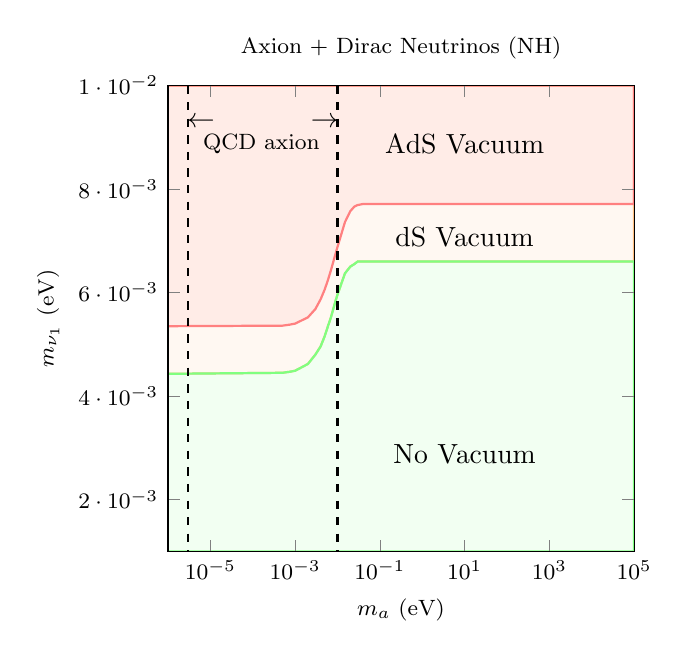
\begin{tikzpicture}
		\begin{semilogxaxis}	[height=7.5cm,
		width=7.5cm, axis on top, ticklabel style = {font=\footnotesize},
		 xmin=0.000001,   xmax=100000,
		ymin=0.001,   ymax=0.01,title={{\footnotesize Axion + Dirac Neutrinos (NH)}},
		xlabel={\footnotesize $m_a$ (eV)},ylabel={\footnotesize $m_{\nu_1}$ (eV)},
		%xtick=\empty,
		%ytick=\empty  
		scaled y ticks=false,
		]
		\addplot[color=orange!50!white, fill=orange!50!white, fill opacity=0.1, thick, mark=none] coordinates {
		(0.000001,     0.00443)
		(0.0005,     0.00445)
		(0.00075,    0.00447)
		(0.001,       0.00449)
		(0.002,      0.00462)
		(0.003,      0.0048)
		(0.004,      0.00496)
		(0.005,      0.00516)
		(0.006,      0.00536)
		(0.007,      0.00552)
		(0.008,       0.00569)
		(0.009,      0.00584)
		(0.010,      0.00596)
		(0.015,      0.00637)
		(0.020,      0.0065)
		(0.025,      0.00655)
		(0.030,      0.0066)
		(0.035,       0.0066)
		(0.040,      0.0066)
		(0.050,      0.0066)
		(0.100,      0.0066)
		(100000,      0.0066)
		(100000,     0.01)
		(0.000001,     0.01)
		};
		\addplot[color=red!50!white, fill=red!50!white, fill opacity=0.1, thick, mark=none] coordinates {
(0.000001,  0.00535)
(0.0005,  0.00536)
(0.00075, 0.00538)
(0.001,   0.0054)
(0.002,   0.00552)
(0.003,   0.00568)
(0.004,   0.00587)
(0.005,   0.00606)
(0.006,   0.00625)
(0.007,   0.00643)
(0.008,   0.0066)
(0.009,   0.00675)
(0.010,   0.00688)
(0.015,   0.00736)
(0.020,   0.00757)
(0.025,   0.00766)
(0.030,   0.00769)
(0.035,   0.0077)
(0.040,   0.00771)
(0.050,   0.00771)
(0.100,   0.00771)
(100000,   0.00771)
		(100000,     0.01)
		(0.000001,     0.01)
		};
		\addplot[color=green!50!white, fill=green!50!white, fill opacity=0.1, thick, mark=none] coordinates {
(0.000001,     0.00443)
(0.0005,     0.00445)
(0.00075,    0.00447)
(0.001,       0.00449)
(0.002,      0.00462)
(0.003,      0.0048)
(0.004,      0.00496)
(0.005,      0.00516)
(0.006,      0.00536)
(0.007,      0.00552)
(0.008,       0.00569)
(0.009,      0.00584)
(0.010,      0.00596)
(0.015,      0.00637)
(0.020,      0.0065)
(0.025,      0.00655)
(0.030,      0.0066)
(0.035,       0.0066)
(0.040,      0.0066)
(0.050,      0.0066)
(0.100,      0.0066)
(100000,      0.0066)
(100000,     0.001)
(0.000001,     0.001)
		};
		\addplot[color=black, thick, dashed] coordinates {
		(0.01,0.01)
		(0.01,0.001)
		};
		\addplot[color=black, thick, dashed] coordinates {
		(0.000003,0.01)
		(0.000003,0.001)
		};
		\node[anchor=south, black] at (axis cs:0.005,0.0090) {$\rightarrow$};
		\node[anchor=south, black] at (axis cs:0.000006,0.0090) {$\leftarrow$};
		\node[anchor=south, black] at (axis cs:0.00016,0.0085) {{\footnotesize QCD axion}};
		\node[anchor=south, black] at (axis cs:10,0.0085) {AdS Vacuum};
		\node[anchor=south, black] at (axis cs:10,0.0067) {dS Vacuum};
		\node[anchor=south, black] at (axis cs:10,0.0025) {No Vacuum};
		\end{semilogxaxis}%
		\end{tikzpicture}%
		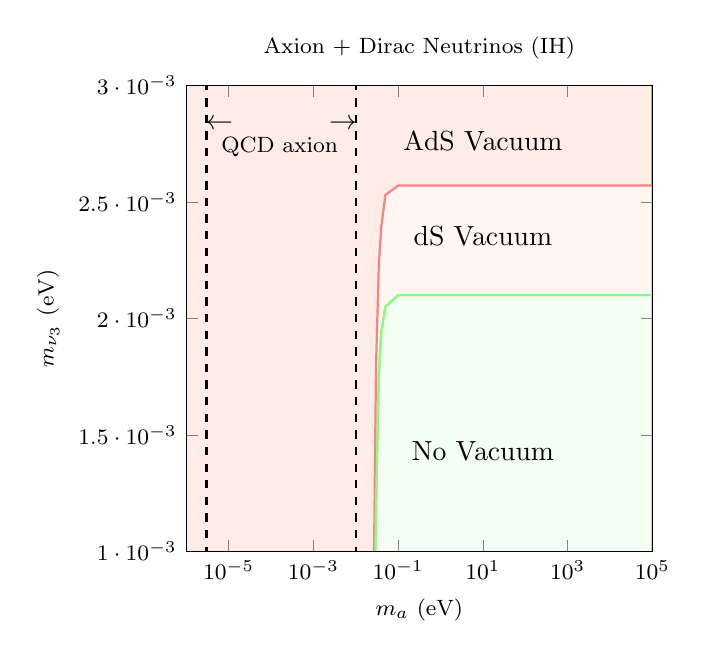
\begin{tikzpicture}
		\begin{semilogxaxis}	[height=7.5cm,
		width=7.5cm, axis on top, ticklabel style = {font=\footnotesize},
		 xmin=0.000001,   xmax=100000,
		ymin=0.001,   ymax=0.003,title={{\footnotesize Axion + Dirac Neutrinos (IH)}},
		xlabel={\footnotesize $m_a$ (eV)},ylabel={\footnotesize $m_{\nu_3}$ (eV)},
		%xtick=\empty,
		%ytick=\empty 
		scaled y ticks=false,
		]
		\addplot[color=orange!50!white, fill=orange!50!white, fill opacity=0.1, thick, mark=none] coordinates {
(0.000001  ,   0.0001)
(0.0005  ,   0.0001)
(0.00075 ,   0.0001)
(0.001   ,    0.0001)
(0.002   ,   0.0001)
(0.003   ,   0.0001)
(0.004   ,   0.0001)
(0.005   ,   0.0001)
(0.006   ,   0.0001)
(0.007   ,   0.0001)
(0.008   ,    0.0001)
(0.009   ,   0.0001)
(0.010   ,   0.0001)
(0.015   ,   0.0001)
(0.020  ,   0.0001)
(0.025   ,   0.0001)
(0.030   ,   0.00120)
(0.035   ,    0.00176)
(0.040   ,   0.00194)
(0.050   ,   0.00205)
(0.100   ,   0.0021)
(100000   ,   0.0021)
		(100000,     0.01)
		(0.000001,     0.01)
		};
		\addplot[color=red!50!white, fill=red!50!white, fill opacity=0.1, thick, mark=none] coordinates {
(0.000001,  0.0001)
(0.0005 , 0.0001)
(0.00075, 0.0001)
(0.001  , 0.0001)
(0.002  , 0.0001)
(0.003  , 0.0001)
(0.004  , 0.0001)
(0.005  , 0.0001)
(0.006  , 0.0001)
(0.007  , 0.0001)
(0.008  , 0.0001)
(0.009  , 0.0001)
(0.010  , 0.0001)
(0.015  , 0.0001)
(0.020  , 0.0001)
(0.025  , 0.00042)
(0.030  , 0.001795)
(0.035  , 0.002234)
(0.040  , 0.002392)
(0.050  , 0.00253)
(0.100  , 0.00257)
(100000  , 0.00257)
		(100000,     0.01)
		(0.000001,     0.01)
		};
		\addplot[color=green!50!white, fill=green!50!white, fill opacity=0.1, thick, mark=none] coordinates {
(0.000001  ,   0.0001)
(0.0005  ,   0.0001)
(0.00075 ,   0.0001)
(0.001   ,    0.0001)
(0.002   ,   0.0001)
(0.003   ,   0.0001)
(0.004   ,   0.0001)
(0.005   ,   0.0001)
(0.006   ,   0.0001)
(0.007   ,   0.0001)
(0.008   ,    0.0001)
(0.009   ,   0.0001)
(0.010   ,   0.0001)
(0.015   ,   0.0001)
(0.020  ,   0.0001)
(0.025   ,   0.0001)
(0.030   ,   0.00120)
(0.035   ,    0.00176)
(0.040   ,   0.00194)
(0.050   ,   0.00205)
(0.100   ,   0.0021)
(100000   ,   0.0021)
(100000,     0.0001)
(0.000001,     0.0001)
		};
		\addplot[color=black, thick, dashed] coordinates {
		(0.01,0.01)
		(0.01,0.001)
		};
		\addplot[color=black, thick, dashed] coordinates {
		(0.000003,0.01)
		(0.000003,0.001)
		};
		\node[anchor=south, black] at (axis cs:0.005,0.00277) {$\rightarrow$};
		\node[anchor=south, black] at (axis cs:0.000006,0.00277) {$\leftarrow$};
		\node[anchor=south, black] at (axis cs:0.00016,0.00265) {{\footnotesize QCD axion}};
		\node[anchor=south, black] at (axis cs:10,0.00268) {AdS Vacuum};
		\node[anchor=south, black] at (axis cs:10,0.00227) {dS Vacuum};
		\node[anchor=south, black] at (axis cs:10,0.00135) {No Vacuum};
		\end{semilogxaxis}%
		\end{tikzpicture}%
		\caption{\footnotesize Contour plots for the appeareance of different kind of vacua in the mass of the lightest neutrino - mass of the axion plane when we have $n=0$ and there is no flux term affecting the potential. The range of the QCD axion is shown as an area delimited with dashed lines. On the left panel the case of NH is shown. For every mass of the axion we can find a bound on the lightest neutrino mass for which we can evade the AdS vacuum. On the right panel the case of IH is shown. In this case when the axion has a mass smaller than $m_a\leq 30$ meV, an AdS vacuum is formed.}
		\label{fig:neuaxion}
	\end{center}
\end{figure}



If $n=0$ then only the mass term in Eq.~\eqref{eq:axiontotal} contributes to the effective potential. So the bounds on the neutrino sector could be different for different choices of axino masses.

Concerning the case of Majorana neutrinos, we found that no vacua different from AdS could be achieved. If we include a term for the axion, as it is a boson its contribution is negative so it will make the AdS vacua deeper for Majorana neutrinos. 

In the case of Dirac neutrinos, the negative contribution of the axion could change some kind of vacua, some of them could also change its nature or even create new vacua where there was not any. For masses of the axion smaller than the ones of the AdS limit in Tab.~\ref{tab:dirac}, \textit{i.e.} $m_a< 10^{-3}$ eV, a constant term $-r^3/720\pi R^6$ is seen, as if the axion is a massless particle, so the vacuum are shifted the same height in this range of masses. For masses larger than $10^{-3}$ eV the mass of the axion is important and affect the vacua of the neutrinos. However, when the axion mass is large enough there is no contribution that affects to the effective potential of the neutrinos. Nonetheless this behaviour depends also in the internal hierarchy of the neutrino masses. In NH the two lightest neutrinos are close in mass and there is one that is heavier, on the other hand for IH the two closest in mass neutrinos are the heavy ones, and this will have an impact also for different masses of the axion.

In Fig.~\ref{fig:neuaxion}\footnote{\Mnote{I have not included any constraint in the axion mass range since I am not familiar with them.}} the effect of the axion for the different vacua formation is shown in the lightest neutrino mass and axion mass plane. For this plot we have assumed that $n=0$ so there is no contribution from the flux term. We have analysed masses of the axion from $10^{-6}$ eV to $10^{5}$ eV. We can see the  different effects that an axion could produce for NH and IH hierarchies:

\begin{table}
\begin{center}
\begin{tabular}{|c | c | c |}
$m_a$ & NH & IH \\
 \hline
$\lesssim 10^{-4}$ eV & $m_{\nu_1}> 5.35$ meV & $m_{\nu_3}>0.0$ meV\\
$10^{-3}$ eV & $m_{\nu_1}> 5.4$ meV& $m_{\nu_3}>0.0$ meV\\
$10^{-2}$ eV & $m_{\nu_1}> 6.87$ meV & $m_{\nu_3}>0.0$ meV\\
$\gtrsim 10^{-1}$ eV & $m_{\nu_1}> 7.7$ meV & $m_{\nu_3}>2.55$ meV\\
\hline
\end{tabular}
\caption{Upper bound on the lightest neutrino mass for NH and IH up to which an AdS vacuum is formed for different QCD axion masses.}
\label{tab:axion}
\end{center}
\end{table}

\subsubsection*{NH Dirac neutrinos}

In the NH case we realise that for axion masses smaller than $10^{-4}$ eV only the constant term for massless particles is affecting the potential so the same limit in the lightest neutrino mass is found for the axion mass range $m_a=(10^{-6}-10^{-4})$ eV, that is $m_{\nu_1}> 5.35$ meV. For masses of the axion of the same order of this lightest neutrino the limit changes to $m_{\nu_1}> 5.4$ meV for $m_a=1$ meV and $m_{\nu_1}> 6.87$ meV for $m_a=10$ meV. For masses of the axion $m_a > 100$ meV the limit on the lightest neutrino mass is $m_{\nu_1}> 7.7$ meV. For larger masses\footnote{In this range there should be no QCD axion due to astrophysical and cosmological bounds.} the axion field is not affecting the effective potential of the neutrinos since it is more massive than the heavier neutrino ($m_{\nu_3}\sim 50$ meV) so we obtain the same result as in Tab.~\ref{tab:dirac}.

\subsubsection*{IH Dirac neutrinos}

For IH, when we include an axion field an AdS vacuum is created even when the lightest neutrino mass is set to zero, $m_{\nu_3}=0$ eV. The reason for this behaviour is the fact that in IH there are two heavy states that even when the lightest neutrino mass is set to zero their masses are $m_{\nu_1}\sim m_{\nu_2}\sim 50$ meV. In this case there are 5 bosonic degrees of freedom against 4 fermionic ones below 50 meV, so an AdS vacuum is formed. However, when the axion mass reaches the heavy neutrino states masses the fermionic degrees of freedom start contributing to the effective potential. In that sense, when the mass of the lightest neutrino is set to zero, $m_{\nu_3}=0$ eV, one finds that for masses of the axion greater than $m_a>24.8$ meV the AdS vacuum becomes a dS one. For instance, for an axion mass of $m_a=50$ meV or larger the limit of the lightest neutrino mass in order to avoid an AdS vacuum is $m_{\nu_3}=2.5$ meV. 



\subsection{QCD axion}

For the QCD axion one has tipically $f_a=10^{8}-10^{12}$ GeV according to astrophysical and cosmological constraints. The QCD axion decay constant could be computed at leading order in chiral perturbation theory using the masses of the up and down quark \cite{diCortona:2015ldu},
\begin{eqnarray}
m_a=\frac{z^{1/2}}{1+z}\frac{f_\pi m_\pi}{f_a},
\end{eqnarray}
where $f_\pi$ and $m_\pi$ are the pion decay constant and pion mass respectively and $z=m_u/m_d$. Following \cite{diCortona:2015ldu}, the mass of the axion can be written,
\begin{eqnarray}
m_a=5.70\,{\rm eV}\,\frac{10^6\,{\rm GeV}}{f_a},
\label{eq:qcdaxion}
\end{eqnarray}
so the mass of the QCD axion lies in the range $m_a=(10^{-6}-10^{-2})$ eV. 

Having such a big values for $f_a$ the flux term of Eq.~\eqref{eq:flux} dominates over the rest and no vacuum is produced. This eliminates any bound on neutrino masses. 

However if one applies the case where $n=0$ then only the Casimir terms applies and a rich phenomenology for the vacuum appear. As astrophysical constraints tell us that the QCD axion lies in the range $(10^{-6}-10^{-2})$ eV, some specific properties could be learnt from here. For NH in the neutrino sector the QCD axion will decrease the upper bound on the lightest neutrino mass up to $~5$ meV. Nonetheless for higher axion masses reaching the limit of $10^{-2}$ eV this bound is weakened up to $~6$ meV. In the case of IH an AdS vacuum is always found for the range of QCD axion masses allowed by the present constraints.




\subsection{Relaxion/Hierarxion}

In principle we have to study these cases also. If we assume the $n=0$ case we can apply the plot of Fig.~\ref{fig:neuaxion}. However, as Luis pointed out here $f_a$ could be smaller than in the QCD axion since the relation of Eq.~\eqref{eq:qcdaxion} does not hold for this kind of axions. In this case we could take into account the flux term and see how it affects to the neutrino sector.

\section{Goldstino/Gravitino contribution}

\begin{figure}[t]
	\begin{center}
		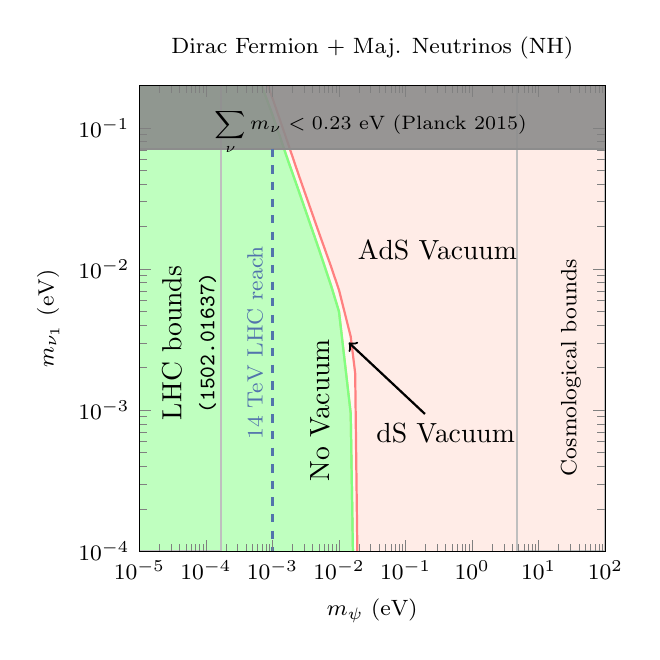
\begin{tikzpicture}
		\begin{loglogaxis}	[height=7.5cm,
		width=7.5cm, axis on top, ticklabel style = {font=\footnotesize},
		 xmin=0.00001 ,   xmax=100,
		ymin=0.0001,   ymax=0.2,title={{\footnotesize Dirac Fermion + Maj. Neutrinos (NH)}},
		xlabel={\footnotesize $m_{\psi}$ (eV)},ylabel={\footnotesize $m_{\nu_1}$ (eV)},
		%xtick=\empty,
		%ytick=\empty  
		scaled y ticks=false,
		]
		\addplot[color=orange!50!white, fill=orange!50!white, fill opacity=0.1, thick, mark=none] coordinates {
		(0.00017,  1.113)
		(0.00025,  0.725)
		(0.0005,  0.309)
		(0.00075,  0.179)
		(0.00090,  0.142)
		(0.001,  0.124)
(0.0017,  0.0595)
(0.0025,  0.0355)
(0.005, 0.0138)
(0.0075,   0.0078)
(0.01,   0.005)
(0.015,   0.00095)
(0.0175,   0.00001)
(0.02,   0.00001)
(10.0,   0.00001)
		(100,     0.00001)
		(100,     20.0)
		(0.00017,  20.0)
		};
		\addplot[color=red!50!white, fill=red!50!white, fill opacity=0.1, thick, mark=none] coordinates {
		(0.00017,  1.6131)
		(0.00025,  0.947)
		(0.0005,  0.405)
		(0.00075,  0.24)
		(0.00090,  0.186)
		(0.001, 0.1627)
(0.0017,  0.0785)
(0.0025,  0.0459)
(0.005, 0.01808)
(0.0075,   0.0106)
(0.01,   0.0071)
(0.015,   0.00332)
(0.0175,   0.00183)
(0.02,   0.00001)
(10.0,   0.00001)
		(100,     0.00001)
		(100,     20.0)
		(0.00017,  20.0)
		};
		\addplot[color=green!50!white, fill=green!50!white, fill opacity=0.5, thick, mark=none] coordinates {
		(0.00001,  1.113)
		(0.00025,  0.725)
		(0.0005,  0.309)
		(0.00075,  0.179)
		(0.00090,  0.142)
		(0.001,  0.124)
(0.0017,  0.0595)
(0.0025,  0.0355)
(0.005, 0.0138)
(0.0075,   0.0078)
(0.01,   0.005)
(0.015,   0.00095)
(0.0175,   0.00001)
(0.02,   0.00001)
(10.0,   0.00001)
		(100,     0.00001)
		(100,     0.000001)
		(0.00001,  0.000001)
		};
		\addplot[color=gray!50!white, %fill=gray!50!white, fill opacity=0.5,
		 thick, mark=none] coordinates {
(0.00017,  10.0)
(0.00017,  0.0001)
(0.00001,  0.0001)
(0.00001,  10.1)
		};
		\addplot[color=gray!50!white, %fill=gray!50!white, fill opacity=0.9, 
		thick, mark=none] coordinates {
(4.7,  10.1)
(4.7,  0.0001)
(100,  0.0001)
(100,  10.1)
		};
		\addplot[color=gray!90!white, fill=gray!90!white, fill opacity=0.9, thick, mark=none] coordinates {
		(0.00001,  10.1)
		(0.00001,  0.0711939)
		(100,  0.0711939)
		(100,  10.1)
		};
		\node[anchor=south, black, rotate=90] at (axis cs:60,0.002) {\footnotesize Cosmological bounds};
		\node[anchor=south, black, rotate=90] at (axis cs:0.00006,0.003) {LHC bounds};
		\node[anchor=south, black, rotate=90] at (axis cs:0.0002,0.003) {\footnotesize \tt (1502.01637)};
		\node[anchor=south, black, rotate=0] at (axis cs:0.03,0.055) {\scriptsize $\displaystyle \sum_{\nu} m_\nu < 0.23$ eV (Planck 2015)};
		\node[anchor=south, black, rotate=0] (source) at (axis cs:0.3,0.01) {AdS Vacuum};
		\node[anchor=south, black, rotate=90] (source) at (axis cs:0.01,0.001) {No Vacuum};
		\node[anchor=south, black, rotate=0] (source) at (axis cs:0.4,0.0005) {dS Vacuum};
		\node (destination) at (axis cs:0.01,0.0035){};
		\draw[->, thick](source)--(destination);
		%\addplot[color=black, thick, densely dashed] coordinates {
		%(0.00017,10.1)
		%(0.00017,0.0001)
		%};
		%\addplot[color=black, thick, dashed] coordinates {
		%(0.000084,10.1)
		%(0.000084,0.0001)
		%};
		\addplot[color=myblue, thick, dashed] coordinates {
		(0.001,0.0711939)
		(0.001,0.0001)
		};
		\node[anchor=south, myblue, rotate=90] at (axis cs:0.001,0.003) {\footnotesize 14 TeV LHC reach};
%		\node[anchor=south, black] at (axis cs:0.005,0.0090) {$\rightarrow$};
%		\node[anchor=south, black] at (axis cs:0.000006,0.0090) {$\leftarrow$};
%		\node[anchor=south, black] at (axis cs:0.00016,0.0085) {{\footnotesize QCD axion}};
%		\node[anchor=south, black] at (axis cs:10,0.0085) {AdS Vacuum};
%		\node[anchor=south, black] at (axis cs:10,0.0067) {dS Vacuum};
%		\node[anchor=south, black] at (axis cs:10,0.0025) {No Vacuum};
		\end{loglogaxis}%
		\end{tikzpicture}%
		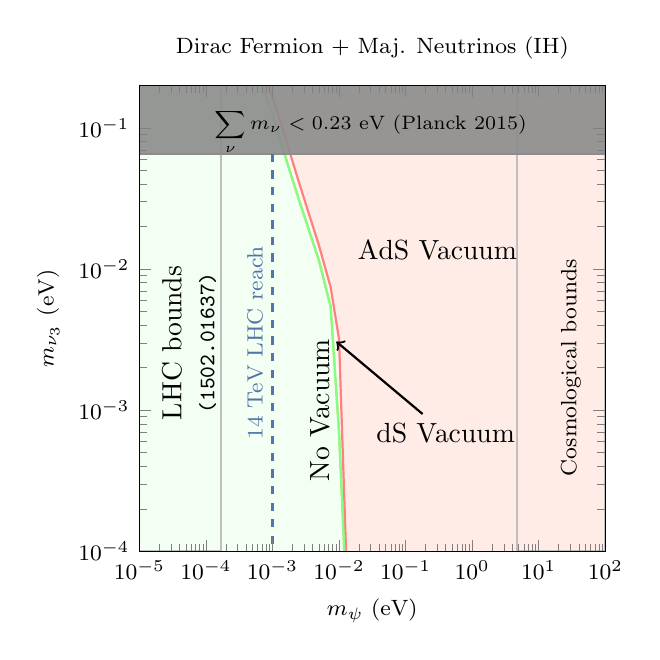
\begin{tikzpicture}
		\begin{loglogaxis}	[height=7.5cm,
				width=7.5cm, axis on top, ticklabel style = {font=\footnotesize},
				 xmin=0.00001 ,   xmax=100,
				 		ymin=0.0001,   ymax=0.2,title={{\footnotesize Dirac Fermion + Maj. Neutrinos (IH)}},
				xlabel={\footnotesize $m_{\psi}$ (eV)},ylabel={\footnotesize $m_{\nu_3}$ (eV)},
				%xtick=\empty,
				%ytick=\empty  
				scaled y ticks=false,
				]
		\addplot[color=orange!50!white, fill=orange!50!white, fill opacity=0.1, thick, mark=none] coordinates {
(0.00017,1.11)
(0.00025,0.73)
(0.0005,0.31)
(0.00075,0.182)
(0.001,0.127)
(0.0017,  0.055)
(0.0025,  0.031)
(0.005, 0.0115)
(0.0075,   0.0054)
(0.01,   0.0007)
(0.015,   0.00001)
(0.0175,   0.00001)
(0.02,   0.00001)
(10.0,   0.00001)
		(100,     0.00001)
		(100,     10.2)
		(0.00017,  10.2)
		};
		\addplot[color=red!50!white, fill=red!50!white, fill opacity=0.1, thick, mark=none] coordinates {
(0.00017,1.5148)
(0.00025,1.38726)
(0.0005,0.4043)
(0.00075,0.2472)
(0.001,0.1655)
(0.0017,  0.0748)
(0.0025,  0.0412)
(0.005, 0.0147)
(0.0075,   0.00742)
(0.01,   0.0032)
(0.015,   0.00001)
(0.0175,   0.00001)
(0.02,   0.00001)
(10.0,   0.00001)
		(100,     0.00001)
		(100,     10.2)
		(0.00017,  10.2)
		};
		\addplot[color=green!50!white, fill=green!50!white, fill opacity=0.1, thick, mark=none] coordinates {
(0.00001,1.11)
(0.00025,0.73)
(0.0005,0.31)
(0.00075,0.182)
(0.001,0.127)
(0.0017,  0.055)
(0.0025,  0.031)
(0.005, 0.0115)
(0.0075,   0.0054)
(0.01,   0.0007)
(0.015,   0.00001)
(0.0175,   0.00001)
(0.02,   0.00001)
(10.0,   0.00001)
		(100,     0.00001)
		(100,     0.000001)
		(0.00001,  0.000001)
		};
		\addplot[color=gray!50!white, %fill=gray!50!white, fill opacity=0.5, 
		thick, mark=none] coordinates {
(0.00017,  10.0)
(0.00017,  0.0001)
(0.00001,  0.0001)
(0.00001,  10.1)
		};
		\addplot[color=gray!50!white, %fill=gray!50!white, fill opacity=0.9, 
		thick, mark=none] coordinates {
(4.7,  10.1)
(4.7,  0.0001)
(100,  0.0001)
(100,  10.1)
		};
		\addplot[color=gray!90!white, fill=gray!90!white, fill opacity=0.9, thick, mark=none] coordinates {
		(0.00001,  10.1)
		(0.00001,  0.0655118)
		(100,  0.0655118)
		(100,  10.1)
		};
		\node[anchor=south, black, rotate=90] at (axis cs:60,0.002) {\footnotesize Cosmological bounds};
		\node[anchor=south, black, rotate=90] at (axis cs:0.00006,0.003) {LHC bounds};
		\node[anchor=south, black, rotate=90] at (axis cs:0.0002,0.003) {\footnotesize \tt (1502.01637)};
		\node[anchor=south, black, rotate=0] at (axis cs:0.03,0.055) {\scriptsize $\displaystyle \sum_{\nu} m_\nu < 0.23$ eV (Planck 2015)};
		%\addplot[color=black, thick, dashed] coordinates {
		%(0.00017,10.1)
		%(0.00017,0.0001)
		%};
		%\addplot[color=black, thick, dashed] coordinates {
		%(0.000084,10.1)
		%(0.000084,0.0001)
		%};
		\addplot[color=myblue, thick, dashed] coordinates {
		(0.001,0.0655118)
		(0.001,0.0001)
		};
		\node[anchor=south, myblue, rotate=90] at (axis cs:0.001,0.003) {\footnotesize 14 TeV LHC reach};
		\node[anchor=south, black, rotate=0] (source) at (axis cs:0.3,0.01) {AdS Vacuum};
		\node[anchor=south, black, rotate=90] (source) at (axis cs:0.01,0.001) {No Vacuum};
		\node[anchor=south, black, rotate=0] (source) at (axis cs:0.4,0.0005) {dS Vacuum};
		\node (destination) at (axis cs:0.0065,0.0035){};
		\draw[->, thick](source)--(destination);	
		\end{loglogaxis}%
		\end{tikzpicture}%
		\caption{\footnotesize Majorana neutrinos + gravitino.}
		\label{fig:majneugravitino}
	\end{center}
\end{figure}

\begin{eqnarray}
m_{3/2}=\xi\frac{F}{\sqrt{3}M_p}=\xi \left(\frac{\sqrt{F}}{100\,{\rm TeV}}\right)^2\cdot 2.4 \,{\rm eV},
\end{eqnarray}
here $\xi=F_0/F$, where $F_0$ is the fundamental SUSY-breaking auxiliary field scale and $F$ is the spurion auxiliary field in $X=M+\theta^2 F$ auxiliary field coupled to the MSSM, which may be smaller than $F_0$. So, \textit{e.g.} for $\xi=1$ and $F=(10\,{\rm TeV})^2$ one has $m_{3/2}\simeq 2.4 \times 10^{-2}$ eV.

Typical cosmological bounds set an upper bound in the gravitino mass $m_{3/2}\leq 10$ eV while there are several LHC searches setting lower bounds on the mass of the gravitino $m_{3/2}\geq 10^{-5}$ eV. However a detailed study of gravitino searches in the LHC could give a stronger value for the mass of the gravitino $m_{3/2}\geq 1.7\times 10^{-4}$ eV \cite{Maltoni:2015twa} \footnote{This value is obtained assuming the \textit{gravitino EFT}, setting all the scalar sector at 20 TeV.}.


\begin{figure}[t]
	\begin{center}
		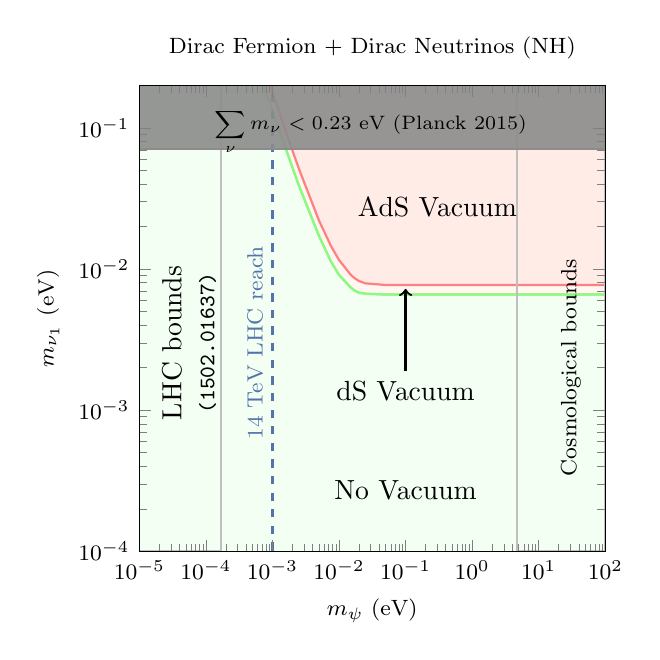
\begin{tikzpicture}
		\begin{loglogaxis}	[height=7.5cm,
		width=7.5cm, axis on top, ticklabel style = {font=\footnotesize},
        xmin=0.00001 ,   xmax=100,
		ymin=0.0001,   ymax=0.2,title={{\footnotesize Dirac Fermion + Dirac Neutrinos (NH)}},
		xlabel={\footnotesize $m_{\psi}$ (eV)},ylabel={\footnotesize $m_{\nu_1}$ (eV)},
		%xtick=\empty,
		%ytick=\empty  
		scaled y ticks=false,
		]
		\addplot[color=orange!50!white, fill=orange!50!white, fill opacity=0.1, thick, mark=none] coordinates {
(0.00017,1.155)
(0.00025,0.76)
(0.0005,0.335)
(0.00075,0.192)
(0.001,0.134)
(0.0017,  0.065)
(0.0025,  0.039)
(0.005, 0.0172)
(0.0075,   0.0114)
(0.01,   0.0091)
(0.015,   0.0074)
(0.0175,   0.0070)
(0.02,   0.0068)
(0.025,  0.0067)
(0.05,   0.0066)
(10.0,   0.0066)
		(100,     0.0066)
		(100,     10.2)
		(0.00017,  10.2)
		};
		\addplot[color=red!50!white, fill=red!50!white, fill opacity=0.1, thick, mark=none] coordinates {
(0.00017,1.5374)
%(0.00025,1.44864)
(0.0005,0.4251)
(0.00075,0.2642)
(0.001,0.178)
(0.0017,  0.08578)
(0.0025,  0.05133)
(0.005, 0.0221)
(0.0075,   0.0147)
(0.01,   0.0116)
(0.015,   0.00911)
(0.0175,   0.00856)
(0.02,   0.00823)
(0.025,  0.00792)
(0.050,  0.00772)
(10.0,   0.00772)
		(100,     0.00772)
		(100,     10.2)
		(0.00017,  10.2)
		};
		\addplot[color=green!50!white, fill=green!50!white, fill opacity=0.1, thick, mark=none] coordinates {
(0.00001,1.155)
(0.00025,0.76)
(0.0005,0.335)
(0.00075,0.192)
(0.001,0.134)
(0.0017,  0.065)
(0.0025,  0.039)
(0.005, 0.0172)
(0.0075,   0.0114)
(0.01,   0.0091)
(0.015,   0.0074)
(0.0175,   0.0070)
(0.02,   0.0068)
(0.025,  0.0067)
(0.05,   0.0066)
(100.0,   0.0066)
		(100,     0.00001)
		(100,     0.000001)
		(0.00001,  0.000001)
		};
		\addplot[color=gray!50!white, %fill=gray!50!white, fill opacity=0.5, 
		thick, mark=none] coordinates {
(0.00017,  10.0)
(0.00017,  0.0001)
(0.00001,  0.0001)
(0.00001,  10.1)
		};
		\addplot[color=gray!50!white, %fill=gray!50!white, fill opacity=0.9, 
		thick, mark=none] coordinates {
(4.7,  10.1)
(4.7,  0.0001)
(100,  0.0001)
(100,  10.1)
		};
		%\addplot[color=black, thick, dashed] coordinates {
		%(0.00017,10.1)
		%(0.00017,0.0001)
		%};
		%\addplot[color=black, thick, dashed] coordinates {
		%(0.000084,10.1)
		%(0.000084,0.0001)
		%};
		\addplot[color=myblue, thick, dashed] coordinates {
		(0.001,10.1)
		(0.001,0.0001)
		};
		\addplot[color=gray!90!white, fill=gray!90!white, fill opacity=0.9, thick, mark=none] coordinates {
		(0.00001,  10.1)
		(0.00001,  0.0711939)
		(100,  0.0711939)
		(100,  10.1)
		};
		\node[anchor=south, black, rotate=90] at (axis cs:60,0.002) {\footnotesize Cosmological bounds};
		\node[anchor=south, black, rotate=90] at (axis cs:0.00006,0.003) {LHC bounds};
		\node[anchor=south, black, rotate=90] at (axis cs:0.0002,0.003) {\footnotesize \tt (1502.01637)};
		\node[anchor=south, black, rotate=0] at (axis cs:0.03,0.055) {\scriptsize $\displaystyle \sum_{\nu} m_\nu < 0.23$ eV (Planck 2015)};
		\node[anchor=south, black, rotate=0] (source) at (axis cs:0.3,0.02) {AdS Vacuum};
		\node[anchor=south, black, rotate=0] (source) at (axis cs:0.1,0.0002) {No Vacuum};
		\node[anchor=south, black, rotate=0] (source) at (axis cs:0.1,0.001) {dS Vacuum};
		\node (destination) at (axis cs:0.1,0.0085){};
		\draw[->, thick](source)--(destination);
		\node[anchor=south, myblue, rotate=90] at (axis cs:0.001,0.003) {\footnotesize 14 TeV LHC reach};
%		\node[anchor=south, black] at (axis cs:0.005,0.0090) {$\rightarrow$};
%		\node[anchor=south, black] at (axis cs:0.000006,0.0090) {$\leftarrow$};
%		\node[anchor=south, black] at (axis cs:0.00016,0.0085) {{\footnotesize QCD axion}};
%		\node[anchor=south, black] at (axis cs:10,0.0085) {AdS Vacuum};
%		\node[anchor=south, black] at (axis cs:10,0.0067) {dS Vacuum};
%		\node[anchor=south, black] at (axis cs:10,0.0025) {No Vacuum};
		\end{loglogaxis}%
		\end{tikzpicture}%
		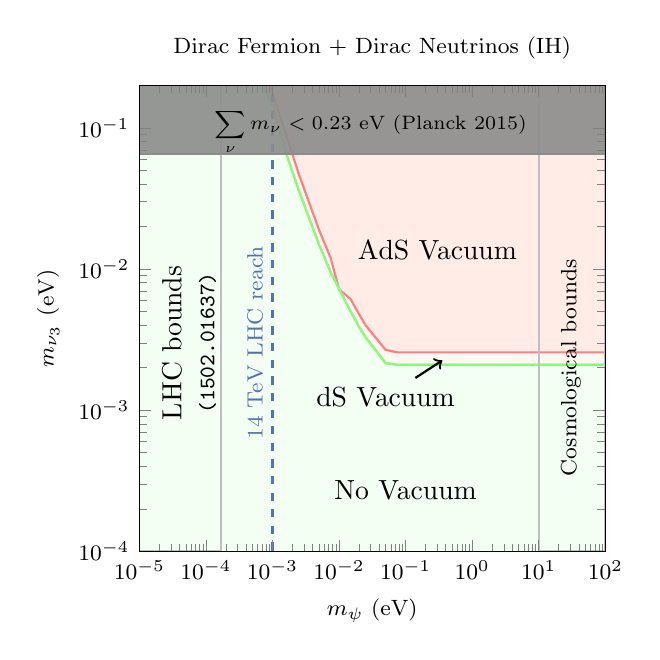
\begin{tikzpicture}
		\begin{loglogaxis}	[height=7.5cm,
				width=7.5cm, axis on top, ticklabel style = {font=\footnotesize},
        xmin=0.00001 ,   xmax=100,
		ymin=0.0001,   ymax=0.2,title={{\footnotesize Dirac Fermion + Dirac Neutrinos (IH)}},
				xlabel={\footnotesize $m_{\psi}$ (eV)},ylabel={\footnotesize $m_{\nu_3}$ (eV)},
				%xtick=\empty,
				%ytick=\empty  
				scaled y ticks=false,
				]
		\addplot[color=orange!50!white, fill=orange!50!white, fill opacity=0.1, thick, mark=none] coordinates {
(0.00017,1.15)
(0.00025,0.75)
(0.0005,0.325)
(0.00075,0.196)
(0.001,0.145)
(0.0017,  0.0612)
(0.0025,  0.036)
(0.005, 0.015)
(0.0075,   0.0095)
%(0.01,   0.0091)
(0.015,   0.005)
(0.0175,  0.0044)
(0.02,   0.0039)
(0.025,  0.0033)
(0.05,   0.00216)
(0.075,  0.0021)
(10.0,   0.0021)
		(100,     0.0021)
		(100,     10.2)
		(0.00017,  10.2)
		};
		\addplot[color=red!50!white, fill=red!50!white, fill opacity=0.1, thick, mark=none] coordinates {
(0.00017,1.5754)
%(0.00025,1.44837)
(0.0005,0.424)
(0.00075,0.2627)
(0.001,0.176)
(0.0017,  0.08175)
(0.0025,  0.0469)
(0.005, 0.019)
(0.0075,   0.01197)
(0.01,   0.0072)
(0.015,   0.00611)
(0.0175,   0.00536)
(0.02,   0.0048)
(0.025,  0.00401)
(0.050,  0.00268)
(0.075,  0.00257)
(10.0,   0.00257)
		(100,     0.00257)
		(100,     10.2)
		(0.00017,  10.2)
		};
		\addplot[color=green!50!white, fill=green!50!white, fill opacity=0.1, thick, mark=none] coordinates {
(0.00001,1.15)
(0.00025,0.75)
(0.0005,0.325)
(0.00075,0.196)
(0.001,0.145)
(0.0017,  0.0612)
(0.0025,  0.036)
(0.005, 0.015)
(0.0075,   0.0095)
%(0.01,   0.0091)
(0.015,   0.005)
(0.0175,  0.0044)
(0.02,   0.0039)
(0.025,  0.0033)
(0.05,   0.00216)
(0.075,  0.0021)
(100.0,   0.0021)
		(100,     0.00001)
		(100,     0.000001)
		(0.00001,  0.000001)
		};
		\addplot[color=gray!50!white, %fill=gray!50!white, fill opacity=0.5, 
		thick, mark=none] coordinates {
(0.00017,  10.0)
(0.00017,  0.0001)
(0.00001,  0.0001)
(0.00001,  10.1)
		};
		\addplot[color=gray!50!white, %fill=gray!50!white, fill opacity=0.9, 
		thick, mark=none] coordinates {
(10,  10.1)
(10,  0.0001)
(100,  0.0001)
(100,  10.1)
		};
		%\addplot[color=black, thick, dashed] coordinates {
		%(0.00017,10.1)
		%(0.00017,0.0001)
		%};
		%\addplot[color=black, thick, dashed] coordinates {
		%(0.000084,10.1)
		%(0.000084,0.0001)
		%};
		\addplot[color=myblue, thick, dashed] coordinates {
		(0.001,10.1)
		(0.001,0.0001)
		};
		\addplot[color=gray!90!white, fill=gray!90!white, fill opacity=0.9, thick, mark=none] coordinates {
		(0.00001,  10.1)
		(0.00001,  0.0655118)
		(100,  0.0655118)
		(100,  10.1)
		};
		\node[anchor=south, black, rotate=90] at (axis cs:60,0.002) {\footnotesize Cosmological bounds};
		\node[anchor=south, black, rotate=90] at (axis cs:0.00006,0.003) {LHC bounds};
		\node[anchor=south, black, rotate=90] at (axis cs:0.0002,0.003) {\footnotesize \tt (1502.01637)};
		\node[anchor=south, black, rotate=0] at (axis cs:0.03,0.055) {\scriptsize $\displaystyle \sum_{\nu} m_\nu < 0.23$ eV (Planck 2015)};
		\node[anchor=south, black, rotate=0] (source) at (axis cs:0.3,0.01) {AdS Vacuum};
		\node[anchor=south, black, rotate=0] (source) at (axis cs:0.1,0.0002) {No Vacuum};
		\node[anchor=south, black, rotate=0] (source) at (axis cs:0.05,0.0009) {dS Vacuum};
		\node (destination) at (axis cs:0.5,0.0025){};
		\draw[->, thick](source)--(destination);
		\node[anchor=south, myblue, rotate=90] at (axis cs:0.001,0.003) {\footnotesize 14 TeV LHC reach};
%		\addplot[color=myblue, thick, dashed] coordinates {
%		(0.00001,0.15)
%		(100,0.15)
%		};
		\end{loglogaxis}%
		\end{tikzpicture}%
		\caption{\footnotesize Dirac neutrinos + gravitino .}
		\label{fig:dirneugravitino}
	\end{center}
\end{figure}

\newpage

\begin{figure}[t]
	\begin{center}
		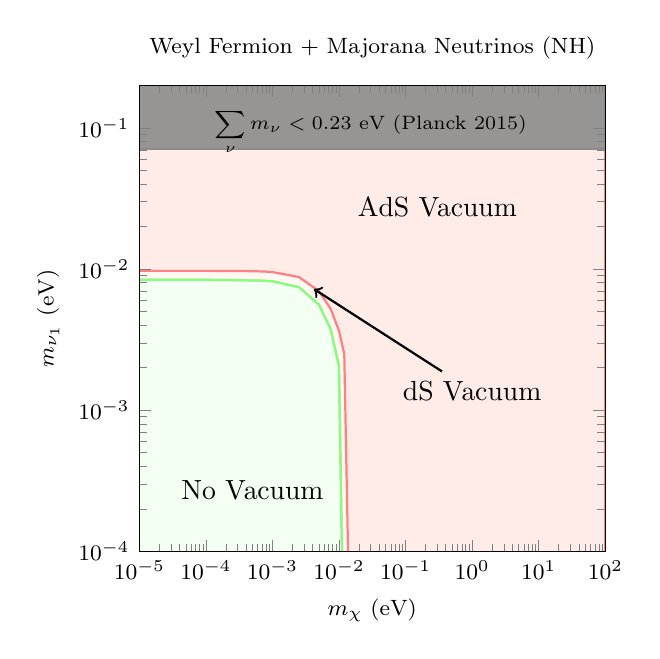
\begin{tikzpicture}
		\begin{loglogaxis}	[height=7.5cm,
		width=7.5cm, axis on top, ticklabel style = {font=\footnotesize},
        xmin=0.00001 ,   xmax=100,
		ymin=0.0001,   ymax=0.2,title={{\footnotesize Weyl Fermion + Majorana Neutrinos (NH)}},
		xlabel={\footnotesize $m_{\chi}$ (eV)},ylabel={\footnotesize $m_{\nu_1}$ (eV)},
		%xtick=\empty,
		%ytick=\empty  
		scaled y ticks=false,
		]
		\addplot[color=orange!50!white, fill=orange!50!white, fill opacity=0.1, thick, mark=none] coordinates {
(0.00001,0.0084)
(0.00005,0.0084)
(0.000075,0.0084)
(0.0001,0.0084)
(0.00025,0.00835)
(0.0005,0.00831)
(0.00075,0.00827)
(0.001,0.0082)
(0.0025,  0.00745)
(0.005, 0.0056)
(0.0075,  0.00375)
(0.01,   0.00205)
(0.012,  0.00001)
(0.015,  0.00001)
(0.0175,   0.00001)
(0.02,   0.00001)
(0.025,  0.00001)
(0.050,  0.00001)
(10.0,   0.00001)
		(100,     0.00001)
		(100,     10.2)
		(0.00001,  10.2)
		};
		\addplot[color=red!50!white, fill=red!50!white, fill opacity=0.1, thick, mark=none] coordinates {
(0.00001,0.00971)
(0.00005,0.00971)
(0.000075,0.00971)
(0.0001,0.00971)
(0.00025,0.0097)
(0.0005,0.00966)
(0.00075,0.00961)
(0.001,0.00953)
(0.0025,  0.00878)
(0.005, 0.00698)
(0.0075,   0.00522)
(0.01,   0.00365)
(0.012,   0.0025)
(0.015,   0.00001)
(0.0175,   0.00001)
(0.02,   0.00001)
(0.025,  0.00001)
(0.050,  0.00001)
(10.0,   0.00001)
		(100,     0.00001)
		(100,     10.2)
		(0.00001,  10.2)
		};
		\addplot[color=green!50!white, fill=green!50!white, fill opacity=0.1, thick, mark=none] coordinates {
(0.00001,0.0084)
(0.00005,0.0084)
(0.000075,0.0084)
(0.0001,0.0084)
(0.00025,0.00835)
(0.0005,0.00831)
(0.00075,0.00827)
(0.001,0.0082)
(0.0025,  0.00745)
(0.005, 0.0056)
(0.0075,  0.00375)
(0.01,   0.00205)
(0.012,  0.00001)
(0.015,  0.00001)
(0.0175,   0.00001)
(0.02,   0.00001)
(0.025,  0.00001)
(0.050,  0.00001)
(10.0,   0.00001)
		(100,     0.00001)
		(100,     0.000001)
		( 0.000001,  0.000001)
		};
%		\addplot[color=gray!50!white, fill=gray!50!white, fill opacity=0.5, thick, mark=none] coordinates {
%(0.00017,  10.0)
%(0.00017,  0.0001)
%(0.00001,  0.0001)
%(0.00001,  10.1)
%		};
%		\addplot[color=gray!50!white, fill=gray!50!white, fill opacity=0.9, thick, mark=none] coordinates {
%(10,  10.1)
%(10,  0.0001)
%(100,  0.0001)
%(100,  10.1)
%		};
		%\addplot[color=black, thick, dashed] coordinates {
		%(0.00017,10.1)
		%(0.00017,0.0001)
		%};
		%\addplot[color=black, thick, dashed] coordinates {
		%(0.000084,10.1)
		%(0.000084,0.0001)
		%};
%		\addplot[color=myblue, thick, dashed] coordinates {
%		(0.001,10.1)
%		(0.001,0.0001)
%		};
		\addplot[color=gray!90!white, fill=gray!90!white, fill opacity=0.9, thick, mark=none] coordinates {
		(0.00001,  10.1)
		(0.00001,  0.0711939)
		(100,  0.0711939)
		(100,  10.1)
		};
%		\node[anchor=south, black, rotate=90] at (axis cs:60,0.002) {\footnotesize Cosmological bounds};
%		\node[anchor=south, black, rotate=90] at (axis cs:0.00006,0.003) {LHC bounds};
%		\node[anchor=south, black, rotate=90] at (axis cs:0.0002,0.003) {\footnotesize \tt (1502.01637)};
		\node[anchor=south, black, rotate=0] at (axis cs:0.03,0.055) {\scriptsize $\displaystyle \sum_{\nu} m_\nu < 0.23$ eV (Planck 2015)};
		\node[anchor=south, black, rotate=0] (source) at (axis cs:0.3,0.02) {AdS Vacuum};
		\node[anchor=south, black, rotate=0] (source) at (axis cs:0.0005,0.0002) {No Vacuum};
		\node[anchor=south, black, rotate=0] (source) at (axis cs:1,0.001) {dS Vacuum};
		\node (destination) at (axis cs:0.003,0.008){};
		\draw[->, thick](source)--(destination);
%		\node[anchor=south, myblue, rotate=90] at (axis cs:0.001,0.003) {\footnotesize 14 TeV LHC reach};
%		\node[anchor=south, black] at (axis cs:0.005,0.0090) {$\rightarrow$};
%		\node[anchor=south, black] at (axis cs:0.000006,0.0090) {$\leftarrow$};
%		\node[anchor=south, black] at (axis cs:0.00016,0.0085) {{\footnotesize QCD axion}};
%		\node[anchor=south, black] at (axis cs:10,0.0085) {AdS Vacuum};
%		\node[anchor=south, black] at (axis cs:10,0.0067) {dS Vacuum};
%		\node[anchor=south, black] at (axis cs:10,0.0025) {No Vacuum};
		\end{loglogaxis}%
		\end{tikzpicture}%
		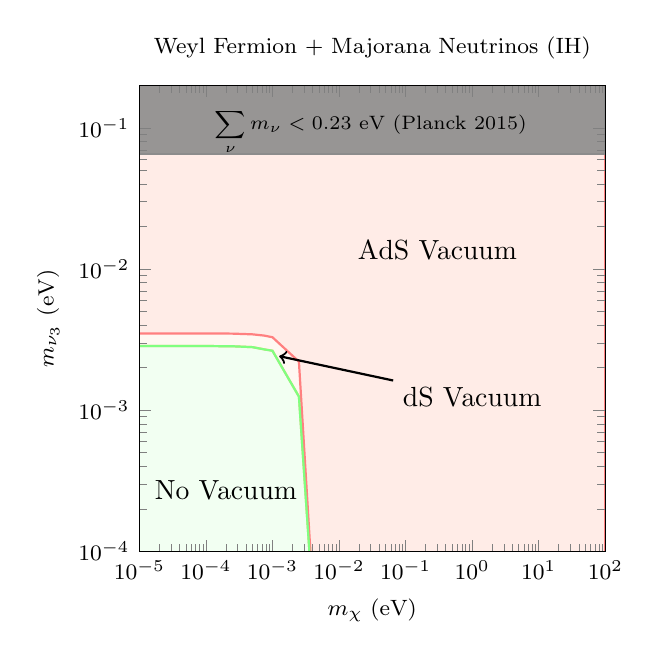
\begin{tikzpicture}
		\begin{loglogaxis}	[height=7.5cm,
				width=7.5cm, axis on top, ticklabel style = {font=\footnotesize},
        xmin=0.00001 ,   xmax=100,
		ymin=0.0001,   ymax=0.2,title={{\footnotesize Weyl Fermion + Majorana Neutrinos (IH)}},
				xlabel={\footnotesize $m_{\chi}$ (eV)},ylabel={\footnotesize $m_{\nu_3}$ (eV)},
				%xtick=\empty,
				%ytick=\empty  
				scaled y ticks=false,
				]
		\addplot[color=orange!50!white, fill=orange!50!white, fill opacity=0.1, thick, mark=none] coordinates {
(0.00001,0.00285)
(0.00005,0.00285)
(0.000075,0.00285)
(0.0001,0.00285)
(0.00025,0.00284)
(0.0005,0.0028)
(0.00075,0.0027)
(0.001,0.00264)
(0.0025,  0.00125)
(0.005, 0.00001)
(0.0075, 0.00001)
(0.01,   0.00001)
(0.012,  0.00001)
(0.015,  0.00001)
(0.0175,   0.00001)
(0.02,   0.00001)
(0.025,  0.00001)
(0.050,  0.00001)
(10.0,   0.00001)
		(100,     0.00001)
		(100,     10.2)
		(0.00001,  10.2)
		};
		\addplot[color=red!50!white, fill=red!50!white, fill opacity=0.1, thick, mark=none] coordinates {
(0.00001,0.0035)
(0.00005,0.0035)
(0.000075,0.0035)
(0.0001,0.0035)
(0.00025,0.00349)
(0.0005,0.00345)
(0.00075,0.00338)
(0.001,0.00329)
(0.0025,  0.00221)
(0.005, 0.00001)
(0.0075, 0.00001)
(0.01,   0.00001)
(0.012,  0.00001)
(0.015,  0.00001)
(0.0175,   0.00001)
(0.02,   0.00001)
(0.025,  0.00001)
(0.050,  0.00001)
(10.0,   0.00001)
		(100,     0.00001)
		(100,     10.2)
		(0.00001,  10.2)
		};
		\addplot[color=green!50!white, fill=green!50!white, fill opacity=0.1, thick, mark=none] coordinates {
(0.00001,0.00285)
(0.00005,0.00285)
(0.000075,0.00285)
(0.0001,0.00285)
(0.00025,0.00284)
(0.0005,0.0028)
(0.00075,0.0027)
(0.001,0.00264)
(0.0025,  0.00125)
(0.005, 0.00001)
(0.0075, 0.00001)
(0.01,   0.00001)
(0.012,  0.00001)
(0.015,  0.00001)
(0.0175,   0.00001)
(0.02,   0.00001)
(0.025,  0.00001)
(0.050,  0.00001)
(10.0,   0.00001)
		(100,     0.00001)
		(100,     0.000001)
		(0.00001,  0.000001)
		};
%		\addplot[color=gray!50!white, fill=gray!50!white, fill opacity=0.5, thick, mark=none] coordinates {
%(0.00017,  10.0)
%(0.00017,  0.0001)
%(0.00001,  0.0001)
%(0.00001,  10.1)
%		};
%		\addplot[color=gray!50!white, fill=gray!50!white, fill opacity=0.9, thick, mark=none] coordinates {
%(10,  10.1)
%(10,  0.0001)
%(100,  0.0001)
%(100,  10.1)
%		};
		%\addplot[color=black, thick, dashed] coordinates {
		%(0.00017,10.1)
		%(0.00017,0.0001)
		%};
		%\addplot[color=black, thick, dashed] coordinates {
		%(0.000084,10.1)
		%(0.000084,0.0001)
		%};
%		\addplot[color=myblue, thick, dashed] coordinates {
%		(0.001,10.1)
%		(0.001,0.0001)
%		};
		\addplot[color=gray!90!white, fill=gray!90!white, fill opacity=0.9, thick, mark=none] coordinates {
		(0.00001,  10.1)
		(0.00001,  0.0655118)
		(100,  0.0655118)
		(100,  10.1)
		};
%		\node[anchor=south, black, rotate=90] at (axis cs:60,0.002) {\footnotesize Cosmological bounds};
%		\node[anchor=south, black, rotate=90] at (axis cs:0.00006,0.003) {LHC bounds};
%		\node[anchor=south, black, rotate=90] at (axis cs:0.0002,0.003) {\footnotesize \tt (1502.01637)};
		\node[anchor=south, black, rotate=0] at (axis cs:0.03,0.055) {\scriptsize $\displaystyle \sum_{\nu} m_\nu < 0.23$ eV (Planck 2015)};
		\node[anchor=south, black, rotate=0] (source) at (axis cs:0.3,0.01) {AdS Vacuum};
		\node[anchor=south, black, rotate=0] (source) at (axis cs:0.0002,0.0002) {No Vacuum};
		\node[anchor=south, black, rotate=0] (source) at (axis cs:1,0.0009) {dS Vacuum};
		\node (destination) at (axis cs:0.0009,0.0025){};
		\draw[->, thick](source)--(destination);
%		\node[anchor=south, myblue, rotate=90] at (axis cs:0.001,0.003) {\footnotesize 14 TeV LHC reach};
%		\addplot[color=myblue, thick, dashed] coordinates {
%		(0.00001,0.15)
%		(100,0.15)
%		};
		\end{loglogaxis}%
		\end{tikzpicture}%
		\caption{\footnotesize Majorana neutrinos + axino .}
		\label{fig:majaxino}
	\end{center}
\end{figure}

\newpage

\begin{figure}[t]
	\begin{center}
		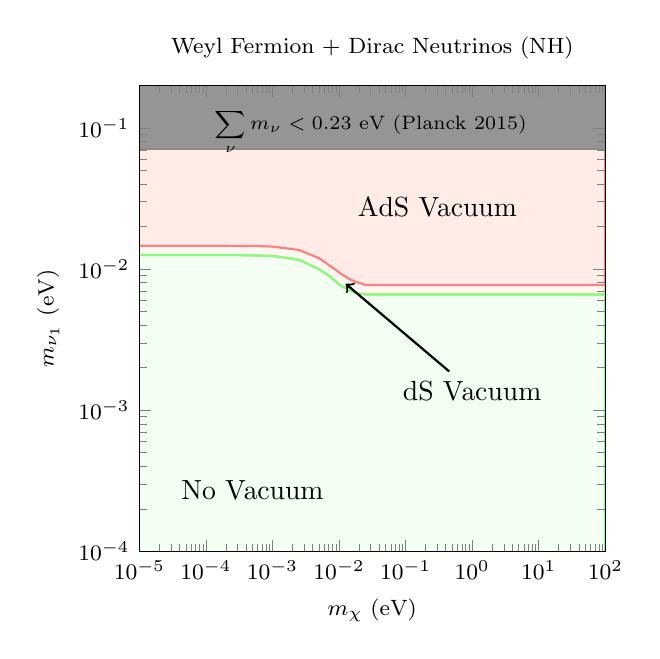
\begin{tikzpicture}
		\begin{loglogaxis}	[height=7.5cm,
		width=7.5cm, axis on top, ticklabel style = {font=\footnotesize},
        xmin=0.00001 ,   xmax=100,
		ymin=0.0001,   ymax=0.2,title={{\footnotesize Weyl Fermion + Dirac Neutrinos (NH)}},
		xlabel={\footnotesize $m_{\chi}$ (eV)},ylabel={\footnotesize $m_{\nu_1}$ (eV)},
		%xtick=\empty,
		%ytick=\empty  
		scaled y ticks=false,
		]
		\addplot[color=orange!50!white, fill=orange!50!white, fill opacity=0.1, thick, mark=none] coordinates {
(0.00001,0.0126)
(0.00005,0.0126)
(0.000075,0.0126)
(0.0001,0.0126)
(0.00025,0.0126)
(0.0005,0.0125)
(0.00075,0.01245)
(0.001,0.0124)
(0.0025,0.01165)
(0.005, 0.01)
(0.0075,  0.0088)
(0.01,   0.0078)
(0.012,  0.0074)
(0.015,  0.007)
(0.0175,   0.0068)
(0.02,   0.0067)
(0.025,  0.0066)
(0.050,  0.0066)
(10.0,   0.0066)
		(100,     0.0066)
		(100,     10.2)
		(0.00001,  10.2)
		};
		\addplot[color=red!50!white, fill=red!50!white, fill opacity=0.1, thick, mark=none] coordinates {
(0.00001,0.01463)
(0.00005,0.01463)
(0.000075,0.01463)
(0.0001,0.01463)
(0.00025,0.0146)
(0.0005,0.01458)
(0.00075,0.01451)
(0.001,0.01442)
(0.0025,  0.01367)
(0.005, 0.01195)
(0.0075,   0.01047)
(0.01,   0.00948)
(0.012,  0.00895)
(0.015,  0.00842)
(0.0175, 0.00815)
(0.02,   0.00799)
(0.025,  0.00772)
(0.050,  0.00772)
(10.0,   0.00772)
		(100,     0.00772)
		(100,     10.2)
		(0.00001,  10.2)
		};
		\addplot[color=green!50!white, fill=green!50!white, fill opacity=0.1, thick, mark=none] coordinates {
(0.00001,0.0126)
(0.00005,0.0126)
(0.000075,0.0126)
(0.0001,0.0126)
(0.00025,0.0126)
(0.0005,0.0125)
(0.00075,0.01245)
(0.001,0.0124)
(0.0025,0.01165)
(0.005, 0.01)
(0.0075,  0.0088)
(0.01,   0.0078)
(0.012,  0.0074)
(0.015,  0.007)
(0.0175,   0.0068)
(0.02,   0.0067)
(0.025,  0.0066)
(0.050,  0.0066)
(10.0,   0.0066)
		(100,     0.0066)
		(100,     0.000001)
		( 0.000001,  0.000001)
		};
%		\addplot[color=gray!50!white, fill=gray!50!white, fill opacity=0.5, thick, mark=none] coordinates {
%(0.00017,  10.0)
%(0.00017,  0.0001)
%(0.00001,  0.0001)
%(0.00001,  10.1)
%		};
%		\addplot[color=gray!50!white, fill=gray!50!white, fill opacity=0.9, thick, mark=none] coordinates {
%(10,  10.1)
%(10,  0.0001)
%(100,  0.0001)
%(100,  10.1)
%		};
		%\addplot[color=black, thick, dashed] coordinates {
		%(0.00017,10.1)
		%(0.00017,0.0001)
		%};
		%\addplot[color=black, thick, dashed] coordinates {
		%(0.000084,10.1)
		%(0.000084,0.0001)
		%};
%		\addplot[color=myblue, thick, dashed] coordinates {
%		(0.001,10.1)
%		(0.001,0.0001)
%		};
		\addplot[color=gray!90!white, fill=gray!90!white, fill opacity=0.9, thick, mark=none] coordinates {
		(0.00001,  10.1)
		(0.00001,  0.0711939)
		(100,  0.0711939)
		(100,  10.1)
		};
%		\node[anchor=south, black, rotate=90] at (axis cs:60,0.002) {\footnotesize Cosmological bounds};
%		\node[anchor=south, black, rotate=90] at (axis cs:0.00006,0.003) {LHC bounds};
%		\node[anchor=south, black, rotate=90] at (axis cs:0.0002,0.003) {\footnotesize \tt (1502.01637)};
		\node[anchor=south, black, rotate=0] at (axis cs:0.03,0.055) {\scriptsize $\displaystyle \sum_{\nu} m_\nu < 0.23$ eV (Planck 2015)};
		\node[anchor=south, black, rotate=0] (source) at (axis cs:0.3,0.02) {AdS Vacuum};
		\node[anchor=south, black, rotate=0] (source) at (axis cs:0.0005,0.0002) {No Vacuum};
		\node[anchor=south, black, rotate=0] (source) at (axis cs:1,0.001) {dS Vacuum};
		\node (destination) at (axis cs:0.009,0.009){};
		\draw[->, thick](source)--(destination);
%		\node[anchor=south, myblue, rotate=90] at (axis cs:0.001,0.003) {\footnotesize 14 TeV LHC reach};
%		\node[anchor=south, black] at (axis cs:0.005,0.0090) {$\rightarrow$};
%		\node[anchor=south, black] at (axis cs:0.000006,0.0090) {$\leftarrow$};
%		\node[anchor=south, black] at (axis cs:0.00016,0.0085) {{\footnotesize QCD axion}};
%		\node[anchor=south, black] at (axis cs:10,0.0085) {AdS Vacuum};
%		\node[anchor=south, black] at (axis cs:10,0.0067) {dS Vacuum};
%		\node[anchor=south, black] at (axis cs:10,0.0025) {No Vacuum};
		\end{loglogaxis}%
		\end{tikzpicture}%
		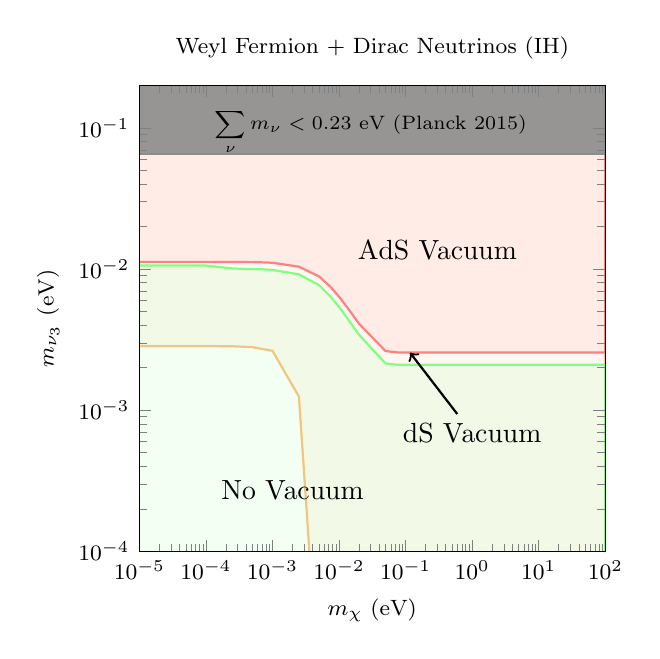
\begin{tikzpicture}
		\begin{loglogaxis}	[height=7.5cm,
				width=7.5cm, axis on top, ticklabel style = {font=\footnotesize},
        xmin=0.00001 ,   xmax=100,
		ymin=0.0001,   ymax=0.2,title={{\footnotesize Weyl Fermion + Dirac Neutrinos (IH)}},
				xlabel={\footnotesize $m_{\chi}$ (eV)},ylabel={\footnotesize $m_{\nu_3}$ (eV)},
				%xtick=\empty,
				%ytick=\empty  
				scaled y ticks=false,
				]
		\addplot[color=orange!50!white, fill=orange!50!white, fill opacity=0.1, thick, mark=none] coordinates {
(0.00001,0.00285)
(0.00005,0.00285)
(0.000075,0.00285)
(0.0001,0.00285)
(0.00025,0.00284)
(0.0005,0.0028)
(0.00075,0.0027)
(0.001,0.00264)
(0.0025,  0.00125)
(0.005, 0.00001)
(0.0075, 0.00001)
(0.01,   0.00001)
(0.012,  0.00001)
(0.015,  0.00001)
(0.0175,   0.00001)
(0.02,   0.00001)
(0.025,  0.00001)
(0.050,  0.00001)
(10.0,   0.00001)
		(100,     0.00001)
		(100,     10.2)
		(0.00001,  10.2)
		};
		\addplot[color=red!50!white, fill=red!50!white, fill opacity=0.1, thick, mark=none] coordinates {
(0.00001,0.01125)
(0.00005,0.01125)
(0.000075,0.01125)
(0.0001,0.01125)
(0.00025,0.01123)
(0.0005,0.0112)
(0.00075,0.01115)
(0.001,0.01109)
(0.0025,0.0104)
(0.005, 0.00888)
(0.0075,0.00746)
(0.01,0.00638)
(0.012,0.0057)
(0.015,0.00496)
(0.0175,0.00447)
(0.02,0.0041)
(0.050,0.002625)
(0.075,0.00257)
(0.1,0.002565)
(10.0,   0.002565)
		(100,     0.002565)
		(100,     10.2)
		(0.00001,  10.2)
		};
		\addplot[color=green!50!white, fill=green!50!white, fill opacity=0.1, thick, mark=none] coordinates {
(0.00001,0.0106)
(0.00005,0.0106)
(0.000075,0.0106)
(0.0001,0.0106)
(0.00025,0.0101)
(0.0005,0.01)
(0.00075,0.00995)
(0.001,0.00986)
(0.0025,0.00918)
(0.005,0.0077)
(0.0075,0.00637)
(0.01,0.0054)
(0.012,0.0048)
(0.015,0.00415)
(0.0175,0.00375)
(0.02,0.00343)
(0.050, 0.002145)
(0.075, 0.0021)
(10.0,  0.0021)
		(100,     0.0021)
		(100,     0.000001)
		(0.00001,  0.000001)
		};
%		\addplot[color=gray!50!white, fill=gray!50!white, fill opacity=0.5, thick, mark=none] coordinates {
%(0.00017,  10.0)
%(0.00017,  0.0001)
%(0.00001,  0.0001)
%(0.00001,  10.1)
%		};
%		\addplot[color=gray!50!white, fill=gray!50!white, fill opacity=0.9, thick, mark=none] coordinates {
%(10,  10.1)
%(10,  0.0001)
%(100,  0.0001)
%(100,  10.1)
%		};
		%\addplot[color=black, thick, dashed] coordinates {
		%(0.00017,10.1)
		%(0.00017,0.0001)
		%};
		%\addplot[color=black, thick, dashed] coordinates {
		%(0.000084,10.1)
		%(0.000084,0.0001)
		%};
%		\addplot[color=myblue, thick, dashed] coordinates {
%		(0.001,10.1)
%		(0.001,0.0001)
%		};
		\addplot[color=gray!90!white, fill=gray!90!white, fill opacity=0.9, thick, mark=none] coordinates {
		(0.00001,  10.1)
		(0.00001,  0.0655118)
		(100,  0.0655118)
		(100,  10.1)
		};
%		\node[anchor=south, black, rotate=90] at (axis cs:60,0.002) {\footnotesize Cosmological bounds};
%		\node[anchor=south, black, rotate=90] at (axis cs:0.00006,0.003) {LHC bounds};
%		\node[anchor=south, black, rotate=90] at (axis cs:0.0002,0.003) {\footnotesize \tt (1502.01637)};
		\node[anchor=south, black, rotate=0] at (axis cs:0.03,0.055) {\scriptsize $\displaystyle \sum_{\nu} m_\nu < 0.23$ eV (Planck 2015)};
		\node[anchor=south, black, rotate=0] (source) at (axis cs:0.3,0.01) {AdS Vacuum};
		\node[anchor=south, black, rotate=0] (source) at (axis cs:0.002,0.0002) {No Vacuum};
		\node[anchor=south, black, rotate=0] (source) at (axis cs:1,0.0005) {dS Vacuum};
		\node (destination) at (axis cs:0.09,0.003){};
		\draw[->, thick](source)--(destination);
%		\node[anchor=south, myblue, rotate=90] at (axis cs:0.001,0.003) {\footnotesize 14 TeV LHC reach};
%		\addplot[color=myblue, thick, dashed] coordinates {
%		(0.00001,0.15)
%		(100,0.15)
%		};
		\end{loglogaxis}%
		\end{tikzpicture}%
		\caption{\footnotesize Dirac neutrinos + axino .}
		\label{fig:diraxino}
	\end{center}
\end{figure}

\newpage

\section{2D stuff}
\subsection{Neutrinos}



\subsection{Axion}

\begin{figure}[t]
	\begin{center}
		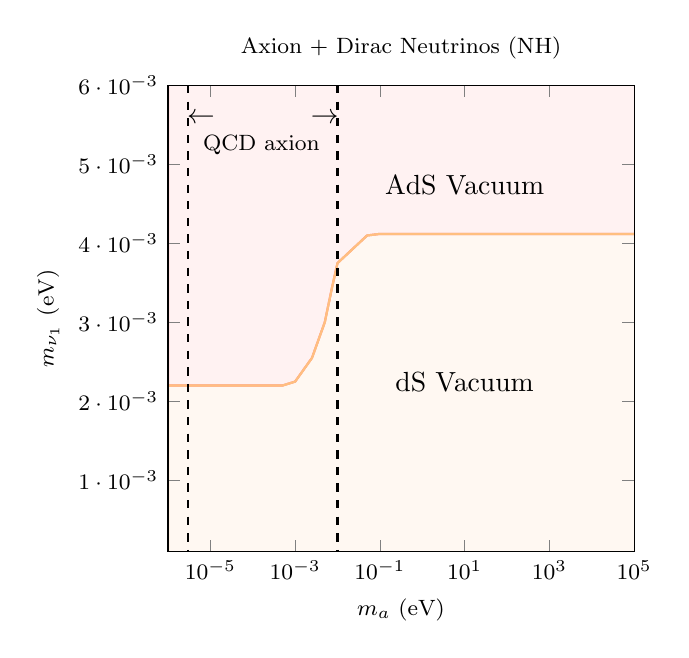
\begin{tikzpicture}
		\begin{semilogxaxis}	[height=7.5cm,
		width=7.5cm, axis on top, ticklabel style = {font=\footnotesize},
		 xmin=0.000001,   xmax=100000,
		ymin=0.0001,   ymax=0.006,title={{\footnotesize Axion + Dirac Neutrinos (NH)}},
		xlabel={\footnotesize $m_a$ (eV)},ylabel={\footnotesize $m_{\nu_1}$ (eV)},
		%xtick=\empty,
		%ytick=\empty  
		scaled y ticks=false,
		]
		\addplot[color=red!50!white, fill=red!50!white, fill opacity=0.1, thick, mark=none] coordinates {

(1e+6,       4.12e-3)		
(1e-1,       4.12e-3)
(5e-2,       4.1e-3)
(1e-2,       3.75e-3)
(7.5e-3,     3.45e-3)
(5e-3,       3.0e-3)
(2.5e-3,     2.55e-3)
(1e-3,       2.25e-3)
(5e-4,       2.2e-3)
(1e-4,       2.2e-3)
(1e-5,       2.2e-3)
(5e-5,       2.2e-3)
(1e-6,       2.2e-3)
(1e-6,       2.2e-1)
(1e+6,       2.2e-1)
		};
		\addplot[color=orange!50!white, fill=orange!50!white, fill opacity=0.1, thick, mark=none] coordinates {
(1e+6,       4.12e-3)		
(1e-1,       4.12e-3)
(5e-2,       4.1e-3)
(1e-2,       3.75e-3)
(7.5e-3,     3.45e-3)
(5e-3,       3.0e-3)
(2.5e-3,     2.55e-3)
(1e-3,       2.25e-3)
(5e-4,       2.2e-3)
(1e-4,       2.2e-3)
(1e-5,       2.2e-3)
(5e-5,       2.2e-3)
(1e-6,       2.2e-3)
(1e-6,       2.2e-5)
(1e+6,       2.2e-5)
		};
		\addplot[color=black, thick, dashed] coordinates {
		(0.01,0.01)
		(0.01,0.00001)
		};
		\addplot[color=black, thick, dashed] coordinates {
		(0.000003,0.01)
		(0.000003,0.00001)
		};
		\node[anchor=south, black] at (axis cs:0.005,0.0054) {$\rightarrow$};
		\node[anchor=south, black] at (axis cs:0.000006,0.0054) {$\leftarrow$};
		\node[anchor=south, black] at (axis cs:0.00016,0.005) {{\footnotesize QCD axion}};
		\node[anchor=south, black] at (axis cs:10,0.0045) {AdS Vacuum};
		\node[anchor=south, black] at (axis cs:10,0.002) {dS Vacuum};
		%\node[anchor=south, black] at (axis cs:10,0.0025) {No Vacuum};
		\end{semilogxaxis}%
		\end{tikzpicture}%
		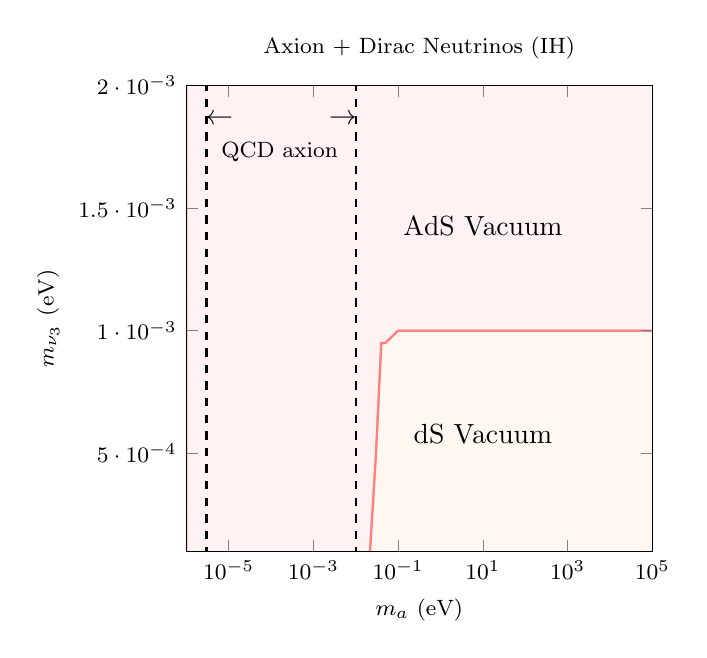
\begin{tikzpicture}
		\begin{semilogxaxis}	[height=7.5cm,
		width=7.5cm, axis on top, ticklabel style = {font=\footnotesize},
		 xmin=0.000001,   xmax=100000,
		ymin=0.0001,   ymax=0.002,title={{\footnotesize Axion + Dirac Neutrinos (IH)}},
		xlabel={\footnotesize $m_a$ (eV)},ylabel={\footnotesize $m_{\nu_3}$ (eV)},
		%xtick=\empty,
		%ytick=\empty 
		scaled y ticks=false,
		]
		\addplot[color=orange!50!white, fill=orange!50!white, fill opacity=0.1, thick, mark=none] coordinates {
(1e+6,   1.0e-3)
(1e-1,   1.0e-3)
(5e-2,   9.5e-4)
(4e-2,   9.5e-4)
(3e-2,   5.0e-4)
(2e-2,   1.0e-6)
(1e-2,   1.0e-6)
(5e-3,   1.0e-6)
(1e-3,   1.0e-6)
(5e-4,   1.0e-6)
(1e-4,   1.0e-6)
(1e-5,   1.0e-6)
(5e-5,   1.0e-6)
(1e-6,   1.0e-6)
(1e+6,   1.0e-6)
		};
		\addplot[color=red!50!white, fill=red!50!white, fill opacity=0.1, thick, mark=none] coordinates {
(1e+6,   1.0e-3)
(1e-1,   1.0e-3)
(5e-2,   9.5e-4)
(4e-2,   9.5e-4)
(3e-2,   5.0e-4)
(2e-2,   1.0e-6)
(1e-2,   1.0e-6)
(5e-3,   1.0e-6)
(1e-3,   1.0e-6)
(5e-4,   1.0e-6)
(1e-4,   1.0e-6)
(1e-5,   1.0e-6)
(5e-5,   1.0e-6)
(1e-6,   1.0e-6)
(1e-6,   1.0e-2)
(1e+6,   1.0e-2)
		};
		\addplot[color=black, thick, dashed] coordinates {
		(0.01,0.01)
		(0.01,0.00001)
		};
		\addplot[color=black, thick, dashed] coordinates {
		(0.000003,0.01)
		(0.000003,0.00001)
		};
		\node[anchor=south, black] at (axis cs:0.005,0.00180) {$\rightarrow$};
		\node[anchor=south, black] at (axis cs:0.000006,0.00180) {$\leftarrow$};
		\node[anchor=south, black] at (axis cs:0.00016,0.00165) {{\footnotesize QCD axion}};
		\node[anchor=south, black] at (axis cs:10,0.00135) {AdS Vacuum};
		\node[anchor=south, black] at (axis cs:10,0.0005) {dS Vacuum};
		%\node[anchor=south, black] at (axis cs:10,0.00135) {No Vacuum};
		\end{semilogxaxis}%
		\end{tikzpicture}%
		\caption{\footnotesize .}
		\label{fig:axion2D}
	\end{center}
\end{figure}



\newpage

\begin{figure}[t]
	\begin{center}
		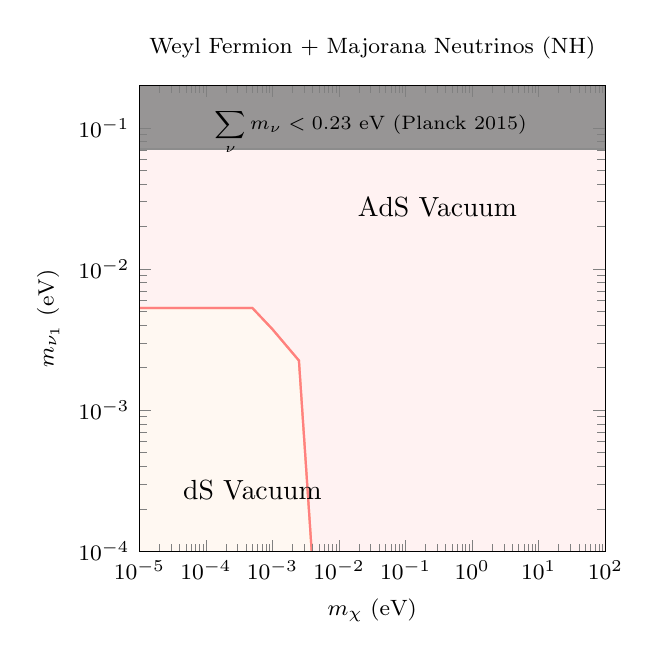
\begin{tikzpicture}
		\begin{loglogaxis}	[height=7.5cm,
		width=7.5cm, axis on top, ticklabel style = {font=\footnotesize},
        xmin=0.00001 ,   xmax=100,
		ymin=0.0001,   ymax=0.2,title={{\footnotesize Weyl Fermion + Majorana Neutrinos (NH)}},
		xlabel={\footnotesize $m_{\chi}$ (eV)},ylabel={\footnotesize $m_{\nu_1}$ (eV)},
		%xtick=\empty,
		%ytick=\empty  
		scaled y ticks=false,
		]
		\addplot[color=orange!50!white, fill=orange!50!white, fill opacity=0.1, thick, mark=none] coordinates {
(1e-1,   1.0e-5)
(5e-2,   1.0e-5)
(1e-2,   1.0e-5)
(5e-3,   1.7e-5)
(2.5e-3, 2.25e-3)
(1e-3,   3.75e-3)
(5e-4,   5.3e-3)
(1e-4,   5.3e-3)
(5e-5,   5.3e-3)
(1e-5,   5.3e-3)
(5e-6,   5.3e-3)
(1e-6,   5.3e-3)
(1e-6,   5.3e-5)
		};
		\addplot[color=red!50!white, fill=red!50!white, fill opacity=0.1, thick, mark=none] coordinates {
(1e-1,   1.0e-5)
(5e-2,   1.0e-5)
(1e-2,   1.0e-5)
(5e-3,   1.7e-5)
(2.5e-3, 2.25e-3)
(1e-3,   3.75e-3)
(5e-4,   5.3e-3)
(1e-4,   5.3e-3)
(5e-5,   5.3e-3)
(1e-5,   5.3e-3)
(5e-6,   5.3e-3)
(1e-6,   5.3e-3)
(1e-6,   5.3e-0)
(1e+3,   5.3e-0)
(1e+3,   1.0e-5)
		};
		\addplot[color=gray!90!white, fill=gray!90!white, fill opacity=0.9, thick, mark=none] coordinates {
		(0.00001,  10.1)
		(0.00001,  0.0711939)
		(100,  0.0711939)
		(100,  10.1)
		};
%		\node[anchor=south, black, rotate=90] at (axis cs:60,0.002) {\footnotesize Cosmological bounds};
%		\node[anchor=south, black, rotate=90] at (axis cs:0.00006,0.003) {LHC bounds};
%		\node[anchor=south, black, rotate=90] at (axis cs:0.0002,0.003) {\footnotesize \tt (1502.01637)};
		\node[anchor=south, black, rotate=0] at (axis cs:0.03,0.055) {\scriptsize $\displaystyle \sum_{\nu} m_\nu < 0.23$ eV (Planck 2015)};
		\node[anchor=south, black, rotate=0] (source) at (axis cs:0.3,0.02) {AdS Vacuum};
		\node[anchor=south, black, rotate=0] (source) at (axis cs:0.0005,0.0002) {dS Vacuum};
%		\node[anchor=south, myblue, rotate=90] at (axis cs:0.001,0.003) {\footnotesize 14 TeV LHC reach};
%		\node[anchor=south, black] at (axis cs:0.005,0.0090) {$\rightarrow$};
%		\node[anchor=south, black] at (axis cs:0.000006,0.0090) {$\leftarrow$};
%		\node[anchor=south, black] at (axis cs:0.00016,0.0085) {{\footnotesize QCD axion}};
%		\node[anchor=south, black] at (axis cs:10,0.0085) {AdS Vacuum};
%		\node[anchor=south, black] at (axis cs:10,0.0067) {dS Vacuum};
%		\node[anchor=south, black] at (axis cs:10,0.0025) {No Vacuum};
		\end{loglogaxis}%
		\end{tikzpicture}%
		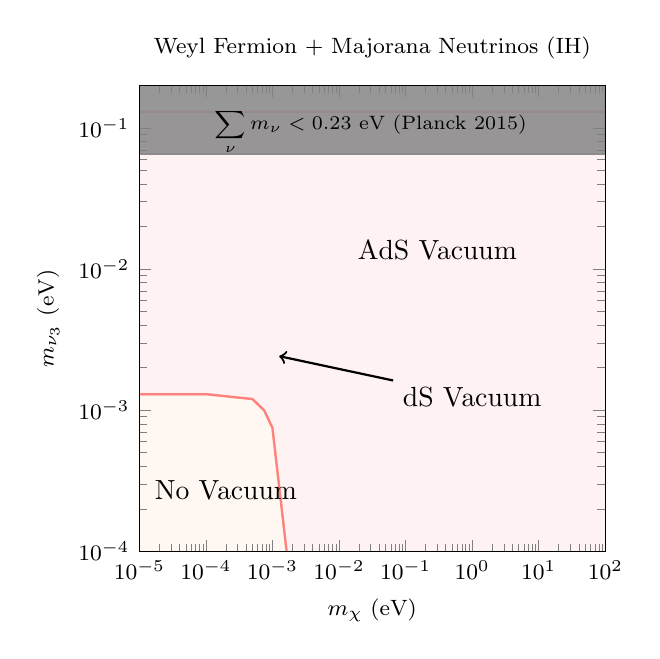
\begin{tikzpicture}
		\begin{loglogaxis}	[height=7.5cm,
				width=7.5cm, axis on top, ticklabel style = {font=\footnotesize},
        xmin=0.00001 ,   xmax=100,
		ymin=0.0001,   ymax=0.2,title={{\footnotesize Weyl Fermion + Majorana Neutrinos (IH)}},
				xlabel={\footnotesize $m_{\chi}$ (eV)},ylabel={\footnotesize $m_{\nu_3}$ (eV)},
				%xtick=\empty,
				%ytick=\empty  
				scaled y ticks=false,
				]
		\addplot[color=orange!50!white, fill=orange!50!white, fill opacity=0.1, thick, mark=none] coordinates {
(1e-1,   1.0e-6)
(5e-2,   1.0e-6)
(1e-2,   1.0e-6)
(5e-3,   1.0e-6)
(1e-3,   7.5e-4)
(7.5e-4, 1.0e-3)
(5e-4,   1.2e-3)
(1e-4,   1.3e-3)
(5e-5,   1.3e-3)
(1e-5,   1.3e-3)
(5e-6,   1.3e-3)
(1e-6,   1.3e-3)
(1e-6,   1.3e-6)
(1e-1,   1.3e-6)
		};
		\addplot[color=red!50!white, fill=red!50!white, fill opacity=0.1, thick, mark=none] coordinates {
(1e-1,   1.0e-6)
(5e-2,   1.0e-6)
(1e-2,   1.0e-6)
(5e-3,   1.0e-6)
(1e-3,   7.5e-4)
(7.5e-4, 1.0e-3)
(5e-4,   1.2e-3)
(1e-4,   1.3e-3)
(5e-5,   1.3e-3)
(1e-5,   1.3e-3)
(5e-6,   1.3e-3)
(1e-6,   1.3e-3)
(1e-6,   1.3e-1)
(1e+3,   1.3e-1)
(1e+3,   1.3e-6)
		};
		\addplot[color=gray!90!white, fill=gray!90!white, fill opacity=0.9, thick, mark=none] coordinates {
		(0.00001,  10.1)
		(0.00001,  0.0655118)
		(100,  0.0655118)
		(100,  10.1)
		};
%		\node[anchor=south, black, rotate=90] at (axis cs:60,0.002) {\footnotesize Cosmological bounds};
%		\node[anchor=south, black, rotate=90] at (axis cs:0.00006,0.003) {LHC bounds};
%		\node[anchor=south, black, rotate=90] at (axis cs:0.0002,0.003) {\footnotesize \tt (1502.01637)};
		\node[anchor=south, black, rotate=0] at (axis cs:0.03,0.055) {\scriptsize $\displaystyle \sum_{\nu} m_\nu < 0.23$ eV (Planck 2015)};
		\node[anchor=south, black, rotate=0] (source) at (axis cs:0.3,0.01) {AdS Vacuum};
		\node[anchor=south, black, rotate=0] (source) at (axis cs:0.0002,0.0002) {No Vacuum};
		\node[anchor=south, black, rotate=0] (source) at (axis cs:1,0.0009) {dS Vacuum};
		\node (destination) at (axis cs:0.0009,0.0025){};
		\draw[->, thick](source)--(destination);
%		\node[anchor=south, myblue, rotate=90] at (axis cs:0.001,0.003) {\footnotesize 14 TeV LHC reach};
%		\addplot[color=myblue, thick, dashed] coordinates {
%		(0.00001,0.15)
%		(100,0.15)
%		};
		\end{loglogaxis}%
		\end{tikzpicture}%
		\caption{\footnotesize Majorana neutrinos + weyl 2D .}
		\label{fig:weylmajorana}
	\end{center}
\end{figure}


\newpage

\begin{figure}[t]
	\begin{center}
		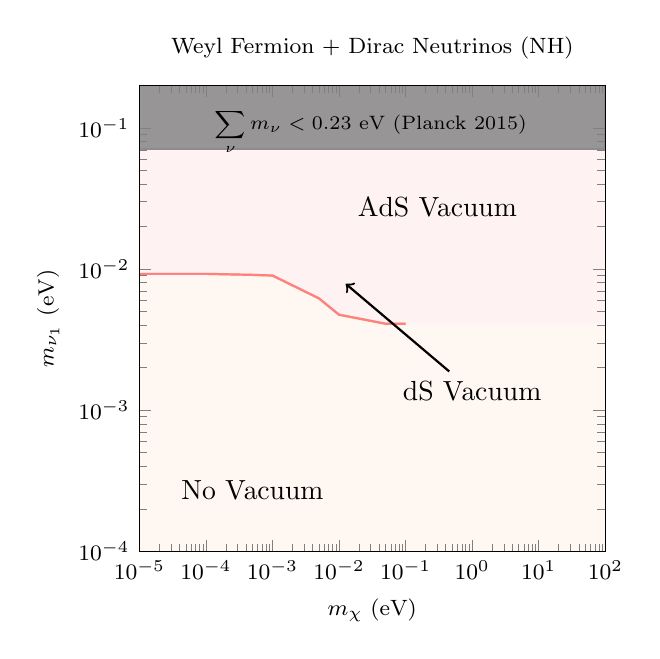
\begin{tikzpicture}
		\begin{loglogaxis}	[height=7.5cm,
		width=7.5cm, axis on top, ticklabel style = {font=\footnotesize},
        xmin=0.00001 ,   xmax=100,
		ymin=0.0001,   ymax=0.2,title={{\footnotesize Weyl Fermion + Dirac Neutrinos (NH)}},
		xlabel={\footnotesize $m_{\chi}$ (eV)},ylabel={\footnotesize $m_{\nu_1}$ (eV)},
		%xtick=\empty,
		%ytick=\empty  
		scaled y ticks=false,
		]
		\addplot[color=orange!50!white, fill=orange!50!white, fill opacity=0.1, thick, mark=none] coordinates {
(1e-1,   4.1e-3)
(5e-2,   4.1e-3)
(1e-2,   4.75e-3)
(5e-3,   6.2e-3)
(1e-3,   9.0e-3)
(5e-4,   9.1e-3)
(1e-4,   9.25e-3)
(5e-5,   9.25e-3)
(1e-5,   9.25e-3)
(5e-6,   9.25e-3)
(1e-6,   9.25e-3)
(1e-6,   9.25e-5)
(1e+3,   9.25e-5)
(1e+3,   4.1e-3)
		};
		\addplot[color=red!50!white, fill=red!50!white, fill opacity=0.1, thick, mark=none] coordinates {
(1e-1,   4.1e-3)
(5e-2,   4.1e-3)
(1e-2,   4.75e-3)
(5e-3,   6.2e-3)
(1e-3,   9.0e-3)
(5e-4,   9.1e-3)
(1e-4,   9.25e-3)
(5e-5,   9.25e-3)
(1e-5,   9.25e-3)
(5e-6,   9.25e-3)
(1e-6,   9.25e-3)
(1e-6,   9.25e-1)
(1e+3,   9.25e-1)
(1e+3,   4.1e-3)
		};
		\addplot[color=gray!90!white, fill=gray!90!white, fill opacity=0.9, thick, mark=none] coordinates {
		(0.00001,  10.1)
		(0.00001,  0.0711939)
		(100,  0.0711939)
		(100,  10.1)
		};
%		\node[anchor=south, black, rotate=90] at (axis cs:60,0.002) {\footnotesize Cosmological bounds};
%		\node[anchor=south, black, rotate=90] at (axis cs:0.00006,0.003) {LHC bounds};
%		\node[anchor=south, black, rotate=90] at (axis cs:0.0002,0.003) {\footnotesize \tt (1502.01637)};
		\node[anchor=south, black, rotate=0] at (axis cs:0.03,0.055) {\scriptsize $\displaystyle \sum_{\nu} m_\nu < 0.23$ eV (Planck 2015)};
		\node[anchor=south, black, rotate=0] (source) at (axis cs:0.3,0.02) {AdS Vacuum};
		\node[anchor=south, black, rotate=0] (source) at (axis cs:0.0005,0.0002) {No Vacuum};
		\node[anchor=south, black, rotate=0] (source) at (axis cs:1,0.001) {dS Vacuum};
		\node (destination) at (axis cs:0.009,0.009){};
		\draw[->, thick](source)--(destination);
%		\node[anchor=south, myblue, rotate=90] at (axis cs:0.001,0.003) {\footnotesize 14 TeV LHC reach};
%		\node[anchor=south, black] at (axis cs:0.005,0.0090) {$\rightarrow$};
%		\node[anchor=south, black] at (axis cs:0.000006,0.0090) {$\leftarrow$};
%		\node[anchor=south, black] at (axis cs:0.00016,0.0085) {{\footnotesize QCD axion}};
%		\node[anchor=south, black] at (axis cs:10,0.0085) {AdS Vacuum};
%		\node[anchor=south, black] at (axis cs:10,0.0067) {dS Vacuum};
%		\node[anchor=south, black] at (axis cs:10,0.0025) {No Vacuum};
		\end{loglogaxis}%
		\end{tikzpicture}%
		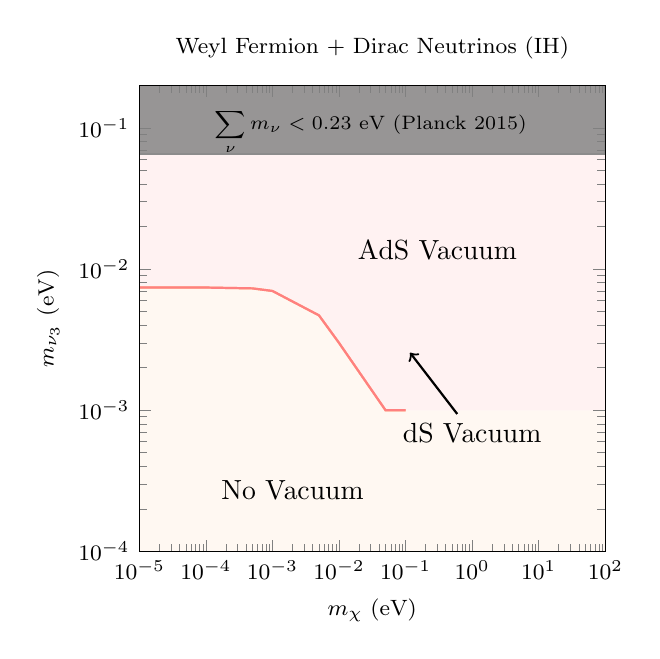
\begin{tikzpicture}
		\begin{loglogaxis}	[height=7.5cm,
				width=7.5cm, axis on top, ticklabel style = {font=\footnotesize},
        xmin=0.00001 ,   xmax=100,
		ymin=0.0001,   ymax=0.2,title={{\footnotesize Weyl Fermion + Dirac Neutrinos (IH)}},
				xlabel={\footnotesize $m_{\chi}$ (eV)},ylabel={\footnotesize $m_{\nu_3}$ (eV)},
				%xtick=\empty,
				%ytick=\empty  
				scaled y ticks=false,
				]
		\addplot[color=orange!50!white, fill=orange!50!white, fill opacity=0.1, thick, mark=none] coordinates {
(1e-1,   1.0e-3)
(5e-2,   1.0e-3)
(1e-2,   3.0e-3)
(5e-3,   4.7e-3)
(1e-3,   7.0e-3)
(5e-4,   7.3e-3)
(1e-4,   7.4e-3)
(5e-5,   7.4e-3)
(1e-5,   7.4e-3)
(5e-6,   7.4e-3)
(1e-6,   7.4e-3)
(1e-6,   7.4e-5)
(1e+3,   7.4e-5)
(1e+3,   1.0e-3)
		};
		\addplot[color=red!50!white, fill=red!50!white, fill opacity=0.1, thick, mark=none] coordinates {
(1e-1,   1.0e-3)
(5e-2,   1.0e-3)
(1e-2,   3.0e-3)
(5e-3,   4.7e-3)
(1e-3,   7.0e-3)
(5e-4,   7.3e-3)
(1e-4,   7.4e-3)
(5e-5,   7.4e-3)
(1e-5,   7.4e-3)
(5e-6,   7.4e-3)
(1e-6,   7.4e-3)
(1e-6,   7.4e-1)
(1e+3,   7.4e-1)
(1e+3,   1.0e-3)
		};
		\addplot[color=gray!90!white, fill=gray!90!white, fill opacity=0.9, thick, mark=none] coordinates {
		(0.00001,  10.1)
		(0.00001,  0.0655118)
		(100,  0.0655118)
		(100,  10.1)
		};
		\node[anchor=south, black, rotate=0] at (axis cs:0.03,0.055) {\scriptsize $\displaystyle \sum_{\nu} m_\nu < 0.23$ eV (Planck 2015)};
		\node[anchor=south, black, rotate=0] (source) at (axis cs:0.3,0.01) {AdS Vacuum};
		\node[anchor=south, black, rotate=0] (source) at (axis cs:0.002,0.0002) {No Vacuum};
		\node[anchor=south, black, rotate=0] (source) at (axis cs:1,0.0005) {dS Vacuum};
		\node (destination) at (axis cs:0.09,0.003){};
		\draw[->, thick](source)--(destination);
%		\node[anchor=south, myblue, rotate=90] at (axis cs:0.001,0.003) {\footnotesize 14 TeV LHC reach};
%		\addplot[color=myblue, thick, dashed] coordinates {
%		(0.00001,0.15)
%		(100,0.15)
%		};
		\end{loglogaxis}%
		\end{tikzpicture}%
		\caption{\footnotesize Dirac neutrinos + weyl 2D .}
		\label{fig:weyldirac}
	\end{center}
\end{figure}

\newpage

\begin{figure}[t]
	\begin{center}
		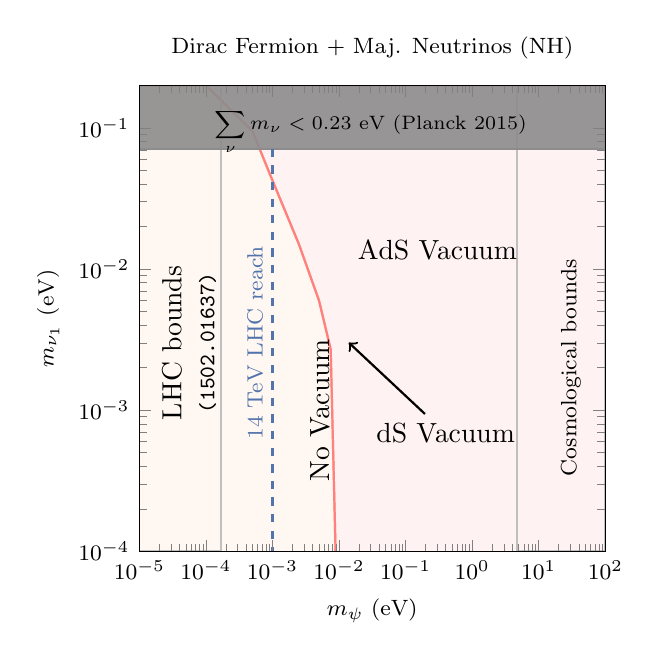
\begin{tikzpicture}
		\begin{loglogaxis}	[height=7.5cm,
		width=7.5cm, axis on top, ticklabel style = {font=\footnotesize},
		 xmin=0.00001 ,   xmax=100,
		ymin=0.0001,   ymax=0.2,title={{\footnotesize Dirac Fermion + Maj. Neutrinos (NH)}},
		xlabel={\footnotesize $m_{\psi}$ (eV)},ylabel={\footnotesize $m_{\nu_1}$ (eV)},
		%xtick=\empty,
		%ytick=\empty  
		scaled y ticks=false,
		]
		\addplot[color=orange!50!white, fill=orange!50!white, fill opacity=0.1, thick, mark=none] coordinates {
(1e-1,   1.0e-5)
(5e-2,   1.0e-5)
(1e-2,   1.0e-5)
(7.5e-3, 2.7e-3) 
(5e-3,   6.0e-3)
(2.5e-3, 1.5e-2)
(1e-3,   4.25e-2)
(5e-4,   9.5e-2)
(1e-4,   2.0e-1)
(5e-5,   2.0e-1)
(1e-5,   2.0e-1)
(5e-6,   2.0e-1)
(1e-6,   2.0e-1)
(1e-6,   2.0e-5)
		};
		\addplot[color=red!50!white, fill=red!50!white, fill opacity=0.1, thick, mark=none] coordinates {
(1e-1,   1.0e-5)
(5e-2,   1.0e-5)
(1e-2,   1.0e-5)
(7.5e-3, 2.7e-3) 
(5e-3,   6.0e-3)
(2.5e-3, 1.5e-2)
(1e-3,   4.25e-2)
(5e-4,   9.5e-2)
(1e-4,   2.0e-1)
(5e-5,   2.0e-1)
(1e-5,   2.0e-1)
(5e-6,   2.0e-1)
(1e-6,   2.0e-1)
(1e+2,   2.0e-1)
(1e+2,   2.0e-5)
		};
		\addplot[color=gray!50!white, %fill=gray!50!white, fill opacity=0.5,
		 thick, mark=none] coordinates {
(0.00017,  10.0)
(0.00017,  0.0001)
(0.00001,  0.0001)
(0.00001,  10.1)
		};
		\addplot[color=gray!50!white, %fill=gray!50!white, fill opacity=0.9, 
		thick, mark=none] coordinates {
(4.7,  10.1)
(4.7,  0.0001)
(100,  0.0001)
(100,  10.1)
		};
		\addplot[color=gray!90!white, fill=gray!90!white, fill opacity=0.9, thick, mark=none] coordinates {
		(0.00001,  10.1)
		(0.00001,  0.0711939)
		(100,  0.0711939)
		(100,  10.1)
		};
		\node[anchor=south, black, rotate=90] at (axis cs:60,0.002) {\footnotesize Cosmological bounds};
		\node[anchor=south, black, rotate=90] at (axis cs:0.00006,0.003) {LHC bounds};
		\node[anchor=south, black, rotate=90] at (axis cs:0.0002,0.003) {\footnotesize \tt (1502.01637)};
		\node[anchor=south, black, rotate=0] at (axis cs:0.03,0.055) {\scriptsize $\displaystyle \sum_{\nu} m_\nu < 0.23$ eV (Planck 2015)};
		\node[anchor=south, black, rotate=0] (source) at (axis cs:0.3,0.01) {AdS Vacuum};
		\node[anchor=south, black, rotate=90] (source) at (axis cs:0.01,0.001) {No Vacuum};
		\node[anchor=south, black, rotate=0] (source) at (axis cs:0.4,0.0005) {dS Vacuum};
		\node (destination) at (axis cs:0.01,0.0035){};
		\draw[->, thick](source)--(destination);
		%\addplot[color=black, thick, densely dashed] coordinates {
		%(0.00017,10.1)
		%(0.00017,0.0001)
		%};
		%\addplot[color=black, thick, dashed] coordinates {
		%(0.000084,10.1)
		%(0.000084,0.0001)
		%};
		\addplot[color=myblue, thick, dashed] coordinates {
		(0.001,0.0711939)
		(0.001,0.0001)
		};
		\node[anchor=south, myblue, rotate=90] at (axis cs:0.001,0.003) {\footnotesize 14 TeV LHC reach};
%		\node[anchor=south, black] at (axis cs:0.005,0.0090) {$\rightarrow$};
%		\node[anchor=south, black] at (axis cs:0.000006,0.0090) {$\leftarrow$};
%		\node[anchor=south, black] at (axis cs:0.00016,0.0085) {{\footnotesize QCD axion}};
%		\node[anchor=south, black] at (axis cs:10,0.0085) {AdS Vacuum};
%		\node[anchor=south, black] at (axis cs:10,0.0067) {dS Vacuum};
%		\node[anchor=south, black] at (axis cs:10,0.0025) {No Vacuum};
		\end{loglogaxis}%
		\end{tikzpicture}%
		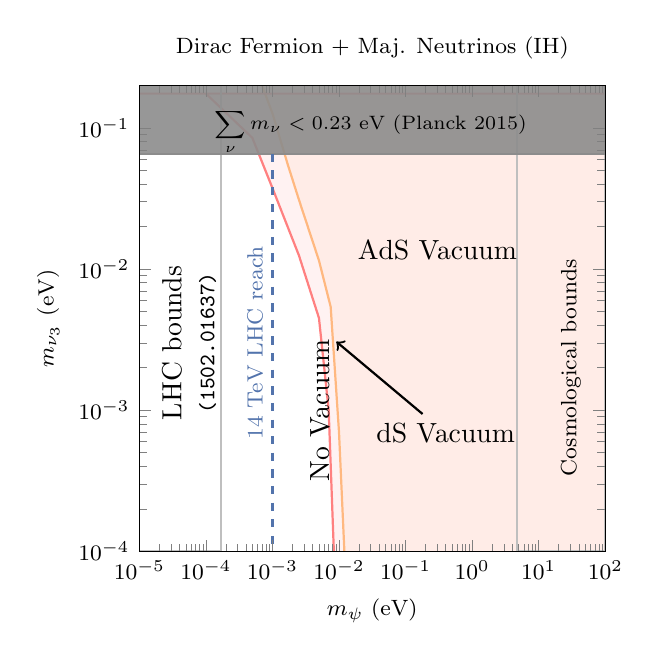
\begin{tikzpicture}
		\begin{loglogaxis}	[height=7.5cm,
				width=7.5cm, axis on top, ticklabel style = {font=\footnotesize},
				 xmin=0.00001 ,   xmax=100,
				 		ymin=0.0001,   ymax=0.2,title={{\footnotesize Dirac Fermion + Maj. Neutrinos (IH)}},
				xlabel={\footnotesize $m_{\psi}$ (eV)},ylabel={\footnotesize $m_{\nu_3}$ (eV)},
				%xtick=\empty,
				%ytick=\empty  
				scaled y ticks=false,
				]
		\addplot[color=orange!50!white, fill=orange!50!white, fill opacity=0.1, thick, mark=none] coordinates {
(0.00017,1.11)
(0.00025,0.73)
(0.0005,0.31)
(0.00075,0.182)
(0.001,0.127)
(0.0017,  0.055)
(0.0025,  0.031)
(0.005, 0.0115)
(0.0075,   0.0054)
(0.01,   0.0007)
(0.015,   0.00001)
(0.0175,   0.00001)
(0.02,   0.00001)
(10.0,   0.00001)
		(100,     0.00001)
		(100,     10.2)
		(0.00017,  10.2)
		};
		\addplot[color=red!50!white, fill=red!50!white, fill opacity=0.1, thick, mark=none] coordinates {
(1e-1,   1.0e-5)
(5e-2,   1.0e-5)
(1e-2,   1.0e-5)
(7.0e-3, 1.0e-3) 
(5e-3,   4.5e-3)
(2.5e-3, 1.25e-2)
(1e-3,   3.75e-2)
(5e-4,   8.5e-2)
(1e-4,   1.75e-1)
(5e-5,   1.75e-1)
(1e-5,   1.75e-1)
(5e-6,   1.75e-1)
(1e-6,   1.75e-1)
(1e+2,   1.75e-1)
(1e+2,   1.75e-5)
		};
		\addplot[color=gray!50!white, %fill=gray!50!white, fill opacity=0.5, 
		thick, mark=none] coordinates {
(0.00017,  10.0)
(0.00017,  0.0001)
(0.00001,  0.0001)
(0.00001,  10.1)
		};
		\addplot[color=gray!50!white, %fill=gray!50!white, fill opacity=0.9, 
		thick, mark=none] coordinates {
(4.7,  10.1)
(4.7,  0.0001)
(100,  0.0001)
(100,  10.1)
		};
		\addplot[color=gray!90!white, fill=gray!90!white, fill opacity=0.9, thick, mark=none] coordinates {
		(0.00001,  10.1)
		(0.00001,  0.0655118)
		(100,  0.0655118)
		(100,  10.1)
		};
		\node[anchor=south, black, rotate=90] at (axis cs:60,0.002) {\footnotesize Cosmological bounds};
		\node[anchor=south, black, rotate=90] at (axis cs:0.00006,0.003) {LHC bounds};
		\node[anchor=south, black, rotate=90] at (axis cs:0.0002,0.003) {\footnotesize \tt (1502.01637)};
		\node[anchor=south, black, rotate=0] at (axis cs:0.03,0.055) {\scriptsize $\displaystyle \sum_{\nu} m_\nu < 0.23$ eV (Planck 2015)};
		%\addplot[color=black, thick, dashed] coordinates {
		%(0.00017,10.1)
		%(0.00017,0.0001)
		%};
		%\addplot[color=black, thick, dashed] coordinates {
		%(0.000084,10.1)
		%(0.000084,0.0001)
		%};
		\addplot[color=myblue, thick, dashed] coordinates {
		(0.001,0.0655118)
		(0.001,0.0001)
		};
		\node[anchor=south, myblue, rotate=90] at (axis cs:0.001,0.003) {\footnotesize 14 TeV LHC reach};
		\node[anchor=south, black, rotate=0] (source) at (axis cs:0.3,0.01) {AdS Vacuum};
		\node[anchor=south, black, rotate=90] (source) at (axis cs:0.01,0.001) {No Vacuum};
		\node[anchor=south, black, rotate=0] (source) at (axis cs:0.4,0.0005) {dS Vacuum};
		\node (destination) at (axis cs:0.0065,0.0035){};
		\draw[->, thick](source)--(destination);	
		\end{loglogaxis}%
		\end{tikzpicture}%
		\caption{\footnotesize Majorana neutrinos + Dirac.}
		\label{fig:majdirac}
	\end{center}
\end{figure}

\newpage

\appendix
\section{Comparison with Arkani Hamed et al. \cite{ArkaniHamed:2007gg}}

In Ref.~\cite{ArkaniHamed:2007gg} Arkani Hamed et al. computed the effective potential when one spatial dimension is compactified in a circle. Here, we reproduce their calculations. Although in the paper they mention the approximation of the effective potential as in Eq.~\eqref{eq:effpotentialapprox}, for the calculations they used the complete expression of the potential in terms of Bessel functions of second order as in Eq.~\eqref{eq:casimirrho}. They assumed a value for the cosmological constant $\Lambda=3.1\cdot 10^{-47}$ GeV$^{4}$. The data they used for the masses of the neutrinos is,
\begin{eqnarray}
\Delta m_{\odot}^2 = (8.0\pm 0.5)\times 10^{-5}\,\, {\rm eV}^2,\\
\Delta m_{\rm atm}^2 = (1.9\div 3.0)\times 10^{-3}\,\, {\rm eV}^2.
\end{eqnarray}
They considered that for NH, $\Delta m_{12}^2=\Delta m^2_{\odot}$ and $\Delta m_{23}^2=\Delta m_{\rm atm}^2$, that means 
\begin{eqnarray}
m_{\nu_1},\quad m_{\nu_2}^2 = m_{\nu_1}^2 + \Delta m_\odot^2,\quad m_{\nu_3}^2= m_{\nu_2}^2 + \Delta m_{\rm atm}^2.
\end{eqnarray}
While for IH they have $\Delta m_{12}^2=\Delta m^2_{\rm atm}$ and $\Delta m_{23}^2=\Delta m_{\odot}^2$, that means 
\begin{eqnarray}
m_{\nu_1},\quad m_{\nu_2}^2 = m_{\nu_1}^2 + \Delta m_{\rm atm}^2,\quad m_{\nu_3}^2= m_{\nu_2}^2 + \Delta m_\odot^2.
\end{eqnarray}

\begin{table}
\begin{center}
\begin{tabular}{c | c | c |}
 & NH & IH \\
 \hline
No vacuum & $m_{\nu_1}< 7.1$ meV & $m_{\nu_1}< 2.5$ meV \\
dS$_3$ vacuum & 7.1 meV $<m_{\nu_1}< 8.3$ meV& 2.5 meV $<m_{\nu_1}<$ 3.1 meV \\
AdS$_3$ vacuum & $m_{\nu_1}> 8.3$ meV & $m_{\nu_1}> 3.1$ meV \\
\hline
\end{tabular}
\caption{Ranges of masses of Dirac neutrinos where different vacua configurations are shown.}
\label{tab:arkani}
\end{center}
\end{table}
We can now reproduce their results. In the left panel of Fig.~\ref{fig:arkani} the effective potential for Majorana neutrinos is shown when $m_{\nu_1}=0$ eV and NH. In the right panel of Fig.~\ref{fig:arkani} the Dirac neutrinos effective potential with NH is shown. Different colours represent different masses of the lightest neutrinos, $m_{\nu_1}=$ 6.5 meV (black), 7.0 meV (green), 7.5 meV (blue), 8.0 meV (brown), and 8.5 meV (red). We also obtained the same numbers for the masses where different vacua are found as it can be seen in Tab.~\ref{tab:arkani}.

Now the results coming from Ref.~\cite{ArkaniHamed:2007gg} can be improved since the data of neutrinos masses has changed. There is also a minor issue about how to defined the masses of the neutrinos according to the NH and IH that is not precise enough in Ref.~\cite{ArkaniHamed:2007gg}. This will be explained in the main text of Section~\ref{sec:neutrinos}.





\begin{figure}[t]
	\begin{center}
		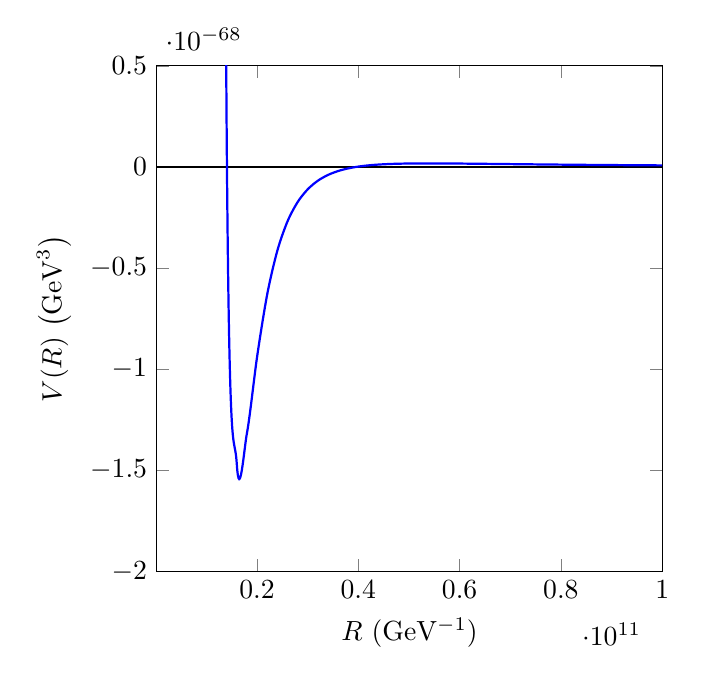
\begin{tikzpicture}
		\begin{axis}	[height=8cm,
		width=8cm,xmin=2.0e+8,   xmax=1.0e+11,
		ymin=-2.0e-68,   ymax=5.0e-69,title={},
		xlabel=$R$ (GeV$^{-1}$),ylabel=$V(R)$ $\left({\rm GeV}^3\right)$,
		%xtick=\empty,
		%ytick=\empty 
		]
		\addplot[color=black] coordinates {
			(2.0e+8,0.0)
			(200000000000,0.0)
		};
		\addplot[color=blue, thick,smooth] coordinates {
%        (10000000000,7.64882544192924e-67)
        (12000000000,1.1529167640889272e-67)
        (14000000000,1.659135412632026e-69)
        (16000000000,-1.4706728252461777e-68)
        (18000000000,-1.3166408335334332e-68)
        (20000000000,-9.398876374383338e-69)
        (22000000000,-6.305321889482771e-69)
        (24000000000,-4.1427881378518663e-69)
        (26000000000,-2.6968880955907055e-69)
        (28000000000,-1.7396725770516592e-69)
        (30000000000,-1.1043708290312178e-69)
        (32000000000,-6.798793514810832e-70)
        (34000000000,-3.9418695389542406e-70)
        (36000000000,-2.0078571800378056e-70)
        (38000000000,-6.944396922851199e-71)
        (40000000000,1.97021786156244e-71)
        (42000000000,7.986633711579006e-71)
        (44000000000,1.19949411758407e-70)
        (46000000000,1.460200978495545e-70)
        (48000000000,1.622628252232169e-70)
        (50000000000,1.7159235585366108e-70)
        (52000000000,1.7605747329741445e-70)
        (54000000000,1.7710958093025875e-70)
        (56000000000,1.757836532347453e-70)
        (58000000000,1.7282158815137163e-70)
        (60000000000,1.687572318857209e-70)
        (62000000000,1.6397559307802378e-70)
        (64000000000,1.587544773754902e-70)
        (66000000000,1.5329402008006318e-70)
        (68000000000,1.477378040005929e-70)
        (70000000000,1.4218807137879063e-70)
        (72000000000,1.367167545534087e-70)
        (74000000000,1.3137352240250276e-70)
        (76000000000,1.2619168093584937e-70)
        (78000000000,1.2119252020537737e-70)
        (80000000000,1.1638852913157922e-70)
        (82000000000,1.1178578064054272e-70)
        (84000000000,1.0738570551430314e-70)
        (86000000000,1.031864137163327e-70)
        (88000000000,9.918367929491799e-71)
        (90000000000,9.537167424495171e-71)
        (92000000000,9.174351444020952e-71)
        (94000000000,8.829166450938377e-71)
        (96000000000,8.500823661996511e-71)
        (98000000000,8.188520935358965e-71)
        (100000000000,7.891458635049884e-71)
        (102000000000,7.608850955772161e-71)
        (104000000000,7.339933829487408e-71)
        (106000000000,7.083970263378512e-71)
        (108000000000,6.840253754077868e-71)
        (110000000000,6.608110268288297e-71)
        (112000000000,6.386899162592398e-71)
        (114000000000,6.176013326049337e-71)
        (116000000000,5.974878761208825e-71)
        (118000000000,5.7829537672747766e-71)
        (120000000000,5.599727849460108e-71)
        (122000000000,5.424720448181291e-71)
        (124000000000,5.257479558449373e-71)
        (126000000000,5.097580291958737e-71)
        (128000000000,4.944623420689644e-71)
        (130000000000,4.798233930360833e-71)
        (132000000000,4.658059604055532e-71)
        (134000000000,4.52376965023247e-71)
        (136000000000,4.395053384688051e-71)
        (138000000000,4.271618972521526e-71)
        (140000000000,4.153192233513722e-71)
        (142000000000,4.039515512361728e-71)
        (144000000000,3.930346613762331e-71)
        (146000000000,3.825457801286334e-71)
        (148000000000,3.7246348582411395e-71)
        (150000000000,3.62767620820814e-71)
        (152000000000,3.5343920926087562e-71)
        (154000000000,3.4446038024547777e-71)
        (156000000000,3.3581429613415527e-71)
        (158000000000,3.2748508567204675e-71)
        (160000000000,3.19457781651987e-71)
        (162000000000,3.1171826282556385e-71)
        (164000000000,3.0425319978720955e-71)
        (166000000000,2.9705000456716874e-71)
        (168000000000,2.9009678368210005e-71)
        (170000000000,2.8338229440558595e-71)
        (172000000000,2.768959040345718e-71)
        (174000000000,2.706275519414226e-71)
        (176000000000,2.645677142146872e-71)
        (178000000000,2.5870737070462192e-71)
        (180000000000,2.530379743019744e-71)
        (182000000000,2.4755142229037682e-71)
        (184000000000,2.422400296239228e-71)
        (186000000000,2.370965039920836e-71)
        (188000000000,2.3211392254405132e-71)
        (190000000000,2.2728571015389852e-71)
        (192000000000,2.226056191166232e-71)
        (194000000000,2.18067710173236e-71)
        (196000000000,2.136663347705684e-71)
        (198000000000,2.0939611846846204e-71)
        (200000000000,2.0525194541347808e-71)
		};
		\end{axis}%
		\end{tikzpicture}%
		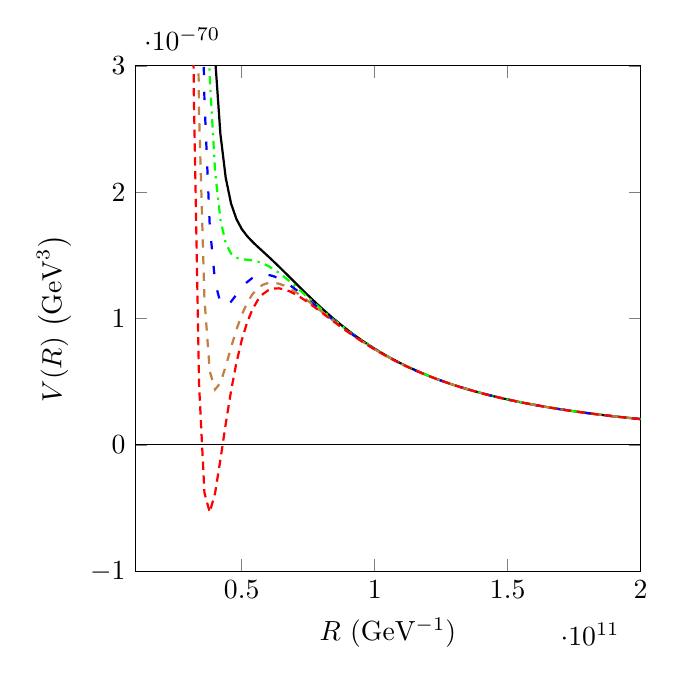
\begin{tikzpicture}
		\begin{axis}	[height=8cm,
		width=8cm,xmin=1.0e+10,   xmax=2.0e+11,
		ymin=-1.0e-70,   ymax=3.0e-70,title={},
		xlabel=$R$ (GeV$^{-1}$),ylabel=$V(R)$ $\left({\rm GeV}^3\right)$,
		%xtick=\empty,
		%ytick=\empty 
		]
		\addplot[color=black] coordinates {
			(10000000000,0.0)
			(200000000000,0.0)
		};
		\addplot[color=black, thick] coordinates {
        (34000000000,9.257224781007743e-70)
        (36000000000,5.974278538188654e-70)
        (38000000000,4.119762983662339e-70)
        (40000000000,3.065159425218237e-70)
        (42000000000,2.4621726629055663e-70)
        (44000000000,2.1148374651925127e-70)
        (46000000000,1.9116910132325966e-70)
        (48000000000,1.7889307923989737e-70)
        (50000000000,1.7099886579295796e-70)
        (52000000000,1.6540078956840087e-70)
        (54000000000,1.6092482180655224e-70)
        (56000000000,1.569267203053745e-70)
        (58000000000,1.5306899936211775e-70)
        (60000000000,1.491899299470214e-70)
        (62000000000,1.4522642903359953e-70)
        (64000000000,1.4116876172469105e-70)
        (66000000000,1.3703412908019884e-70)
        (68000000000,1.3285149850414006e-70)
        (70000000000,1.2865312280725008e-70)
        (72000000000,1.2447001947075149e-70)
        (74000000000,1.203297699916364e-70)
        (76000000000,1.162556528670906e-70)
        (78000000000,1.1226651857522093e-70)
        (80000000000,1.083770542257815e-70)
        (82000000000,1.045982308296332e-70)
        (84000000000,1.0093781421542467e-70)
        (86000000000,9.740087377935372e-71)
        (88000000000,9.39902550435752e-71)
        (90000000000,9.070700071523274e-71)
        (92000000000,8.755071567760222e-71)
        (94000000000,8.451987724698462e-71)
        (96000000000,8.161209502942291e-71)
        (98000000000,7.88243260018817e-71)
        (100000000000,7.615305075414428e-71)
        (102000000000,7.359441660525733e-71)
        (104000000000,7.1144352819315345e-71)
        (106000000000,6.87986625473369e-71)
        (108000000000,6.655309550489622e-71)
        (110000000000,6.440340480771869e-71)
        (112000000000,6.2345390853452445e-71)
        (114000000000,6.037493466647893e-71)
        (116000000000,5.848802271478873e-71)
        (118000000000,5.668076486002943e-71)
        (120000000000,5.4949406808090976e-71)
        (122000000000,5.329033818152625e-71)
        (124000000000,5.170009713020947e-71)
        (126000000000,5.017537222682634e-71)
        (128000000000,4.871300225359043e-71)
        (130000000000,4.730997437118654e-71)
        (132000000000,4.596342106621089e-71)
        (134000000000,4.4670616195786256e-71)
        (136000000000,4.342897038460655e-71)
        (138000000000,4.223602597791969e-71)
        (140000000000,4.1089451711820446e-71)
        (142000000000,3.9987037227974915e-71)
        (144000000000,3.892668753211597e-71)
        (146000000000,3.790641747316243e-71)
        (148000000000,3.692434630165721e-71)
        (150000000000,3.5978692351600894e-71)
        (152000000000,3.5067767878024543e-71)
        (154000000000,3.4189974073265536e-71)
        (156000000000,3.334379627744565e-71)
        (158000000000,3.2527799392743617e-71)
        (160000000000,3.1740623506411296e-71)
        (162000000000,3.0980979723864083e-71)
        (164000000000,3.0247646210386475e-71)
        (166000000000,2.9539464437872334e-71)
        (168000000000,2.8855335631436603e-71)
        (170000000000,2.8194217409582942e-71)
        (172000000000,2.7555120610805194e-71)
        (174000000000,2.693710629896711e-71)
        (176000000000,2.633928293948821e-71)
        (178000000000,2.5760803738216717e-71)
        (180000000000,2.5200864134855574e-71)
        (182000000000,2.465869944289395e-71)
        (184000000000,2.413358262815965e-71)
        (186000000000,2.3624822218327895e-71)
        (188000000000,2.3131760335982406e-71)
        (190000000000,2.265377084811399e-71)
        (192000000000,2.2190257625248475e-71)
        (194000000000,2.1740652903713216e-71)
        (196000000000,2.1304415744872148e-71)
        (198000000000,2.088103058547971e-71)
        (200000000000,2.047000587361913e-71)
		};
		\addplot[color=green, thick,dashdotted] coordinates {
		(34000000000,7.018560428954111e-70)
		(36000000000,4.342710609301919e-70)
		(38000000000,2.915383594569194e-70)
		(40000000000,2.165867393053811e-70)
		(42000000000,1.7836902554567334e-70)
		(44000000000,1.5981050849838034e-70)
		(46000000000,1.5147498991724766e-70)
		(48000000000,1.4815976004860716e-70)
		(50000000000,1.4703022490262407e-70)
		(52000000000,1.4658218838946135e-70)
		(54000000000,1.460576752840737e-70)
		(56000000000,1.4511335656672535e-70)
		(58000000000,1.4363155933372185e-70)
		(60000000000,1.4161261227695942e-70)
		(62000000000,1.3911393887262569e-70)
		(64000000000,1.362161324130145e-70)
		(66000000000,1.3300460919520047e-70)
		(68000000000,1.2956021421277554e-70)
		(70000000000,1.2595491326924701e-70)
		(72000000000,1.2225031323085725e-70)
		(74000000000,1.1849769512812261e-70)
		(76000000000,1.1473880029552283e-70)
		(78000000000,1.1100693750113512e-70)
		(80000000000,1.0732817211405464e-70)
		(82000000000,1.0372247146561129e-70)
		(84000000000,1.0020474605552844e-70)
		(86000000000,9.67857634218837e-71)
		(88000000000,9.347293187313907e-71)
		(90000000000,9.027096179319779e-71)
		(92000000000,8.718241702952756e-71)
		(94000000000,8.420817044575043e-71)
		(96000000000,8.13477775427892e-71)
		(98000000000,7.859978099713902e-71)
		(100000000000,7.596195753415927e-71)
		(102000000000,7.34315170306819e-71)
		(104000000000,7.100526227521982e-71)
		(106000000000,6.867971647868138e-71)
		(108000000000,6.64512244521782e-71)
		(110000000000,6.431603235490241e-71)
		(112000000000,6.227035005482281e-71)
		(114000000000,6.031039942277498e-71)
		(116000000000,5.8432451279020725e-71)
		(118000000000,5.663285321330021e-71)
		(120000000000,5.490805008881643e-71)
		(122000000000,5.3254598703249805e-71)
		(124000000000,5.166917780344392e-71)
		(126000000000,5.014859442429374e-71)
		(128000000000,4.868978733772135e-71)
		(130000000000,4.728982824702948e-71)
		(132000000000,4.594592123922392e-71)
		(134000000000,4.465540090801514e-71)
		(136000000000,4.34157294789702e-71)
		(138000000000,4.222449320225984e-71)
		(140000000000,4.107939822482841e-71)
		(142000000000,3.997826611031318e-71)
		(144000000000,3.891902913977981e-71)
		(146000000000,3.789972549779728e-71)
		(148000000000,3.691849442529953e-71)
		(150000000000,3.5973571402056792e-71)
		(152000000000,3.506328340658014e-71)
		(154000000000,3.4186044289230475e-71)
		(156000000000,3.3340350284648123e-71)
		(158000000000,3.2524775681914065e-71)
		(160000000000,3.1737968664729694e-71)
		(162000000000,3.0978647329063117e-71)
		(164000000000,3.0245595881911053e-71)
		(166000000000,2.953766102186898e-71)
		(168000000000,2.885374849992684e-71)
		(170000000000,2.819281985717943e-71)
		(172000000000,2.755388933485523e-71)
		(174000000000,2.6936020951134333e-71)
		(176000000000,2.633832573857599e-71)
		(178000000000,2.5759959135550302e-71)
		(180000000000,2.520011852481973e-71)
		(182000000000,2.465804091230642e-71)
		(184000000000,2.41330007390792e-71)
		(186000000000,2.362430781967564e-71)
		(188000000000,2.313130540001783e-71)
		(190000000000,2.2653368328371112e-71)
		(192000000000,2.218990133301832e-71)
		(194000000000,2.174033740056862e-71)
		(196000000000,2.1304136249081206e-71)
		(198000000000,2.088078289045335e-71)
		(200000000000,2.0469786276794763e-71)
		};
		\addplot[color=blue, thick, loosely dashed] coordinates {
        (32000000000,8.905939248729686e-70)
        (34000000000,4.8004757941253496e-70)
        (36000000000,2.7346697443619772e-70)
        (38000000000,1.7347028423316397e-70)
        (40000000000,1.28902409979195e-70)
        (42000000000,1.125748812360859e-70)
        (44000000000,1.099774298321279e-70)
        (46000000000,1.1340715181144953e-70)
        (48000000000,1.1885088391005486e-70)
        (50000000000,1.2430181833774776e-70)
        (52000000000,1.2883915069176802e-70)
        (54000000000,1.3212086550536653e-70)
        (56000000000,1.3410340534541837e-70)
        (58000000000,1.348872815401962e-70)
        (60000000000,1.3463308652235687e-70)
        (62000000000,1.3351696962913978e-70)
        (64000000000,1.3170817884802e-70)
        (66000000000,1.2935882311560077e-70)
        (68000000000,1.266002680947862e-70)
        (70000000000,1.2354299989214403e-70)
        (72000000000,1.202781762841144e-70)
        (74000000000,1.1687987954456661e-70)
        (76000000000,1.134075403509183e-70)
        (78000000000,1.0990826181303654e-70)
        (80000000000,1.0641891884245384e-70)
        (82000000000,1.0296798859997877e-70)
        (84000000000,9.957711042327896e-71)
        (86000000000,9.626239467394256e-71)
        (88000000000,9.303550883777258e-71)
        (90000000000,8.9904571485549e-71)
        (92000000000,8.687488354790495e-71)
        (94000000000,8.394952359955021e-71)
        (96000000000,8.112983050115922e-71)
        (98000000000,7.841579335717402e-71)
        (100000000000,7.580636558753992e-71)
        (102000000000,7.329971709927512e-71)
        (104000000000,7.0893436112682265e-71)
        (106000000000,6.858469013510111e-71)
        (108000000000,6.6370353849152915e-71)
        (110000000000,6.424711025105564e-71)
        (112000000000,6.2211530195400655e-71)
        (114000000000,6.026013453602123e-71)
        (116000000000,5.838944226274713e-71)
        (118000000000,5.65960073901832e-71)
        (120000000000,5.487644683106299e-71)
        (122000000000,5.322746106135849e-71)
        (124000000000,5.164584903905078e-71)
        (126000000000,5.012851855836848e-71)
        (128000000000,4.86724929941592e-71)
        (130000000000,4.727491520690754e-71)
        (132000000000,4.59330492296323e-71)
        (134000000000,4.4644280236895334e-71)
        (136000000000,4.340611319808607e-71)
        (138000000000,4.221617053767117e-71)
        (140000000000,4.107218906070632e-71)
        (142000000000,3.99720163497476e-71)
        (144000000000,3.891360679706746e-71)
        (146000000000,3.789501740190517e-71)
        (148000000000,3.6914403434847606e-71)
        (150000000000,3.5970014049113866e-71)
        (152000000000,3.5060187900510213e-71)
        (154000000000,3.4183348823318306e-71)
        (156000000000,3.3338001597722967e-71)
        (158000000000,3.252272783504187e-71)
        (160000000000,3.1736181999551673e-71)
        (162000000000,3.097708757976182e-71)
        (164000000000,3.024423341727928e-71)
        (166000000000,2.953647019770107e-71)
        (168000000000,2.885270710507611e-71)
        (170000000000,2.8191908639237066e-71)
        (172000000000,2.755309159359172e-71)
        (174000000000,2.6935322189677127e-71)
        (176000000000,2.633771336383546e-71)
        (178000000000,2.575942220069958e-71)
        (180000000000,2.5199647507722963e-71)
        (182000000000,2.465762752470788e-71)
        (184000000000,2.4132637762140793e-71)
        (186000000000,2.362398896210507e-71)
        (188000000000,2.313102517558417e-71)
        (190000000000,2.265312195007398e-71)
        (192000000000,2.2189684621575244e-71)
        (194000000000,2.17401467052235e-71)
        (196000000000,2.1303968379024362e-71)
        (198000000000,2.088063505538848e-71)
        (200000000000,2.0469656035396646e-71)
		};
		\addplot[color=brown, thick, dashed] coordinates {
        (32000000000,5.831594829386571e-70)
        (34000000000,2.6147123773562044e-70)
        (36000000000,1.158464543670796e-70)
        (38000000000,5.836008308105056e-71)
        (40000000000,4.3877862010296704e-71)
        (42000000000,4.912563522983561e-71)
        (44000000000,6.218597154582355e-71)
        (46000000000,7.710258334242128e-71)
        (48000000000,9.105690987013952e-71)
        (50000000000,1.0287056328862731e-70)
        (52000000000,1.1220451579869899e-70)
        (54000000000,1.1913006972738143e-70)
        (56000000000,1.2390044658136936e-70)
        (58000000000,1.2683136096478618e-70)
        (60000000000,1.2824088221258824e-70)
        (62000000000,1.2842137308744893e-70)
        (64000000000,1.2762852174757455e-70)
        (66000000000,1.2607920631519876e-70)
        (68000000000,1.2395365884957397e-70)
        (70000000000,1.2139947246547737e-70)
        (72000000000,1.1853615387846844e-70)
        (74000000000,1.1545956743599467e-70)
        (76000000000,1.1224597065509086e-70)
        (78000000000,1.0895553189860646e-70)
        (80000000000,1.0563531964983651e-70)
        (82000000000,1.0232180055574664e-70)
        (84000000000,9.904290313530772e-71)
        (86000000000,9.581970891917884e-71)
        (88000000000,9.26678301948359e-71)
        (90000000000,8.959852758363425e-71)
        (92000000000,8.661961359705928e-71)
        (94000000000,8.373618126116356e-71)
        (96000000000,8.095119041120954e-71)
        (98000000000,7.826593856137592e-71)
        (100000000000,7.568043838921296e-71)
        (102000000000,7.319371979546484e-71)
        (104000000000,7.080407112230807e-71)
        (106000000000,6.8509231340491004e-71)
        (108000000000,6.6306542753719475e-71)
        (110000000000,6.419307193082149e-71)
        (112000000000,6.2165705087564894e-71)
        (114000000000,6.0221222936595336e-71)
        (116000000000,5.835635905241757e-71)
        (118000000000,5.656784501460969e-71)
        (120000000000,5.4852444960474746e-71)
        (122000000000,5.320698166877222e-71)
        (124000000000,5.162835588527208e-71)
        (126000000000,5.0113560269450536e-71)
        (128000000000,4.865968907422982e-71)
        (130000000000,4.726394445480734e-71)
        (132000000000,4.5923640128303174e-71)
        (134000000000,4.463620296512682e-71)
        (136000000000,4.3399172979147105e-71)
        (138000000000,4.2210202091731e-71)
        (140000000000,4.106705197030641e-71)
        (142000000000,3.9967591181923595e-71)
        (144000000000,3.8909791853617334e-71)
        (146000000000,3.789172599201576e-71)
        (148000000000,3.691156158282682e-71)
        (150000000000,3.596755856513264e-71)
        (152000000000,3.5058064754675226e-71)
        (154000000000,3.4181511773590726e-71)
        (156000000000,3.3336411030582223e-71)
        (158000000000,3.2521349784701504e-71)
        (160000000000,3.1734987317236643e-71)
        (162000000000,3.0976051229271447e-71)
        (164000000000,3.0243333876965314e-71)
        (166000000000,2.953568895223009e-71)
        (168000000000,2.8852028213037414e-71)
        (170000000000,2.8191318364897646e-71)
        (172000000000,2.755257809296713e-71)
        (174000000000,2.693487524264546e-71)
        (176000000000,2.6337324145324632e-71)
        (178000000000,2.5759083085068275e-71)
        (180000000000,2.5199351901369745e-71)
        (182000000000,2.4657369722709886e-71)
        (184000000000,2.4132412825368042e-71)
        (186000000000,2.3623792611798704e-71)
        (188000000000,2.313085370284376e-71)
        (190000000000,2.2652972138084364e-71)
        (192000000000,2.2189553678728643e-71)
        (194000000000,2.1740032207567726e-71)
        (196000000000,2.1303868220700525e-71)
        (198000000000,2.08805474059188e-71)
        (200000000000,2.046957930285019e-71)
		};
	    \addplot[color=red, thick, densely dashed] coordinates {
        (30000000000,8.190769321741888e-70)
        (32000000000,2.8006926724815143e-70)
        (34000000000,4.712067164986832e-71)
        (36000000000,-3.790236597123538e-71)
        (38000000000,-5.331750230704275e-71)
        (40000000000,-3.816213777255676e-71)
        (42000000000,-1.175978902275616e-71)
        (44000000000,1.6580207203317829e-71)
        (46000000000,4.265244001949721e-71)
        (48000000000,6.4831689154533805e-71)
        (50000000000,8.276417364709607e-71)
        (52000000000,9.668787183553794e-71)
        (54000000000,1.0708250723146234e-70)
        (56000000000,1.1449346715714058e-70)
        (58000000000,1.1944751828915558e-70)
        (60000000000,1.2241657179023075e-70)
        (62000000000,1.238060749805339e-70)
        (64000000000,1.2395549303942851e-70)
        (66000000000,1.2314422325814508e-70)
        (68000000000,1.2159947239824385e-70)
        (70000000000,1.1950435517260242e-70)
        (72000000000,1.1700540110413622e-70)
        (74000000000,1.1421914854725633e-70)
        (76000000000,1.112377564021992e-70)
        (78000000000,1.0813368531821012e-70)
        (80000000000,1.0496355150125082e-70)
        (82000000000,1.017712711026971e-70)
        (84000000000,9.85906099794272e-71)
        (86000000000,9.544724237208949e-71)
        (88000000000,9.236040803576162e-71)
        (90000000000,8.934424325532259e-71)
        (92000000000,8.640884823546803e-71)
        (94000000000,8.356114205310872e-71)
        (96000000000,8.080554678149354e-71)
        (98000000000,7.814453443271866e-71)
        (100000000000,7.557906383026107e-71)
        (102000000000,7.310892920652338e-71)
        (104000000000,7.0733038020765854e-71)
        (106000000000,6.8449632029818504e-71)
        (108000000000,6.625646286235856e-71)
        (110000000000,6.415093111707048e-71)
        (112000000000,6.2130196218232424e-71)
        (114000000000,6.019126283156668e-71)
        (116000000000,5.8331048497632995e-71)
        (118000000000,5.6546436222565056e-71)
        (120000000000,5.483431503078317e-71)
        (122000000000,5.319161089486036e-71)
        (124000000000,5.161530998474088e-71)
        (126000000000,5.010247579868813e-71)
        (128000000000,4.8650261433065e-71)
        (130000000000,4.7255918002489455e-71)
        (132000000000,4.591680002421373e-71)
        (134000000000,4.4630368421294345e-71)
        (136000000000,4.339419167069626e-71)
        (138000000000,4.220594551886165e-71)
        (140000000000,4.106341160363568e-71)
        (142000000000,3.9964475253898444e-71)
        (144000000000,3.890712268368986e-71)
        (146000000000,3.788943775353599e-71)
        (148000000000,3.690959843607475e-71)
        (150000000000,3.5965873094320603e-71)
        (152000000000,3.5056616657693377e-71)
        (154000000000,3.418026676221252e-71)
        (156000000000,3.333533990617248e-71)
        (158000000000,3.252042766048004e-71)
        (160000000000,3.1734192963090403e-71)
        (162000000000,3.097536651917533e-71)
        (164000000000,3.0242743322425727e-71)
        (166000000000,2.9535179307935674e-71)
        (168000000000,2.8851588143193146e-71)
        (170000000000,2.819093816061729e-71)
        (172000000000,2.7552249432674467e-71)
        (174000000000,2.693459098874389e-71)
        (176000000000,2.6337078171483846e-71)
        (178000000000,2.5758870129384494e-71)
        (180000000000,2.519916744141299e-71)
        (182000000000,2.4657209869104457e-71)
        (184000000000,2.413227423108133e-71)
        (186000000000,2.3623672394756566e-71)
        (188000000000,2.3130749379862162e-71)
        (190000000000,2.2652881568418765e-71)
        (192000000000,2.218947501580467e-71)
        (194000000000,2.173996385767703e-71)
        (196000000000,2.1303808807631437e-71)
        (198000000000,2.0880495740647915e-71)
        (200000000000,2.0469534357552894e-71)
		};
		\end{axis}%
		\end{tikzpicture}%
		\caption{\footnotesize \underline{Left panel}: The effective potential for Majorana neutrinos assuming the lightest neutrino has zero mass and the other have difference in masses $\Delta m_{21}^2$ and $\Delta m_{32}^2$ respectively. In this case we see an AdS vacuum formed by the neutrinos. The increasing in mass makes the vacuum deeper so the possibility of having Majorana neutrinos imply the creation of an AdS vacuum. \underline{Right panel}: The effective potential for Dirac neutrinos assuming the lightest neutrino has a mass of 6.5 meV (black), 7.0 meV (green), 7.5 meV (blue), 8.0 meV (brown) and 8.5 meV (red).}
		\label{fig:arkani}
	\end{center}
\end{figure}

\begin{thebibliography}{99}


\bibitem{ArkaniHamed:2007gg}
  N.~Arkani-Hamed, S.~Dubovsky, A.~Nicolis and G.~Villadoro,
  ``Quantum Horizons of the Standard Model Landscape,''
  JHEP {\bf 0706} (2007) 078
  %doi:10.1088/1126-6708/2007/06/078
  [hep-th/0703067 [HEP-TH]].

\bibitem{Ooguri:2016pdq}
H.~Ooguri and C.~Vafa,
``Non-supersymmetric AdS and the Swampland,''
arXiv:1610.01533 [hep-th].

\bibitem{Olive:2016xmw}
  C.~Patrignani {\it et al.} [Particle Data Group],
  ``Review of Particle Physics,''
  Chin.\ Phys.\ C {\bf 40} (2016) no.10,  100001.

\bibitem{diCortona:2015ldu}
  G.~Grilli di Cortona, E.~Hardy, J.~Pardo Vega and G.~Villadoro,
  ``The QCD axion, precisely,''
  JHEP {\bf 1601} (2016) 034
  [arXiv:1511.02867 [hep-ph]].

\bibitem{Maltoni:2015twa}
  F.~Maltoni, A.~Martini, K.~Mawatari and B.~Oexl,
  ``Signals of a superlight gravitino at the LHC,''
  JHEP {\bf 1504} (2015) 021
  [arXiv:1502.01637 [hep-ph]].
\end{thebibliography}
\end{document} 


\begin{figure}[t]
	\begin{center}
		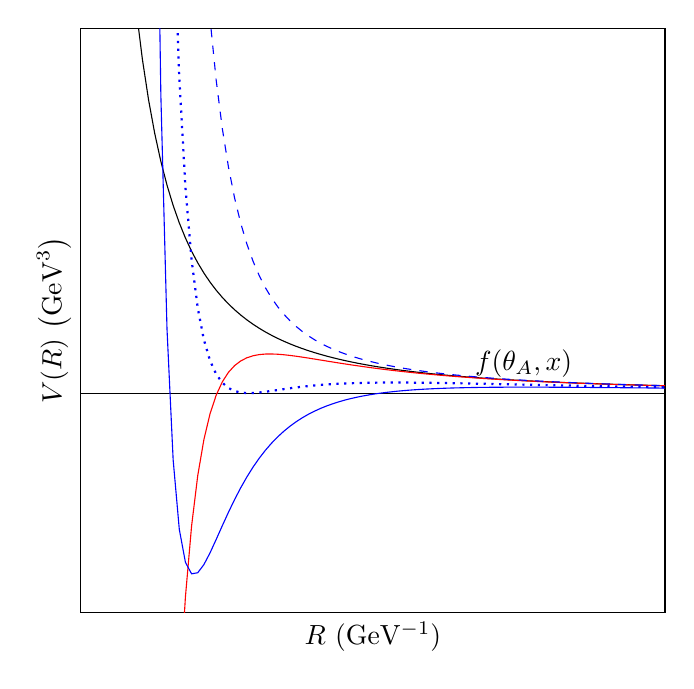
\begin{tikzpicture}
		\begin{axis}	[height=9cm,
		width=9cm,xmin=1.0e+10,   xmax=2.0e+11,
		ymin=-0.6e-69,   ymax=10e-70,title={},
		xlabel=$R$ (GeV$^{-1}$),ylabel=$V(R)$ $\left({\rm GeV}^3\right)$,
		xtick=\empty,
		ytick=\empty 
		]
		\addplot[color=black] coordinates {
			(10000000000,0.0)
			(200000000000,0.0)
		};
		\addplot[color=black] coordinates {
			(10000000000,8.232346170939944e-69)
			(12000000000,5.716907063152738e-69)
			(14000000000,4.2001766178265015e-69)
			(16000000000,3.215760223023416e-69)
			(18000000000,2.5408475836234396e-69)
			(20000000000,2.058086542734986e-69)
			(22000000000,1.7008979692024676e-69)
			(24000000000,1.4292267657881845e-69)
			(26000000000,1.2178026880088674e-69)
			(28000000000,1.0500441544566254e-69)
			(30000000000,9.147051301044382e-70)
			(32000000000,8.03940055755854e-70)
			(34000000000,7.121406722266387e-70)
			(36000000000,6.352118959058599e-70)
			(38000000000,5.701070755498576e-70)
			(40000000000,5.145216356837465e-70)
			(42000000000,4.6668629086961134e-70)
			(44000000000,4.252244923006169e-70)
			(46000000000,3.890522765094491e-70)
			(48000000000,3.5730669144704614e-70)
			(50000000000,3.292938468375977e-70)
			(52000000000,3.0445067200221684e-70)
			(54000000000,2.8231639818038214e-70)
			(56000000000,2.6251103861415634e-70)
			(58000000000,2.4471897059869036e-70)
			(60000000000,2.2867628252610954e-70)
			(62000000000,2.1416093056555525e-70)
			(64000000000,2.009850139389635e-70)
			(66000000000,1.8898866324471865e-70)
			(68000000000,1.7803516805665968e-70)
			(70000000000,1.6800706471306005e-70)
			(72000000000,1.5880297397646498e-70)
			(74000000000,1.5033502868772723e-70)
			(76000000000,1.425267688874644e-70)
			(78000000000,1.3531140977876304e-70)
			(80000000000,1.2863040892093663e-70)
			(82000000000,1.2243227499910684e-70)
			(84000000000,1.1667157271740284e-70)
			(86000000000,1.1130808776284401e-70)
			(88000000000,1.0630612307515423e-70)
			(90000000000,1.0163390334493759e-70)
			(92000000000,9.726306912736227e-71)
			(94000000000,9.31682454837024e-71)
			(96000000000,8.932667286176153e-71)
			(98000000000,8.571789015972455e-71)
			(100000000000,8.232346170939943e-71)
			(102000000000,7.91267413585154e-71)
			(104000000000,7.611266800055421e-71)
			(106000000000,7.32675878510141e-71)
			(108000000000,7.0579099545095536e-71)
			(110000000000,6.803591876809872e-71)
			(112000000000,6.5627759653539085e-71)
			(114000000000,6.334523061665084e-71)
			(116000000000,6.117974264967259e-71)
			(118000000000,5.9123428403762886e-71)
			(120000000000,5.7169070631527385e-71)
			(122000000000,5.531003877277577e-71)
			(124000000000,5.354023264138881e-71)
			(126000000000,5.1854032318845706e-71)
			(128000000000,5.0246253484740875e-71)
			(130000000000,4.8712107520354695e-71)
			(132000000000,4.724716581117966e-71)
			(134000000000,4.584732775083506e-71)
			(136000000000,4.450879201416492e-71)
			(138000000000,4.322803072327213e-71)
			(140000000000,4.200176617826501e-71)
			(142000000000,4.082694986580016e-71)
			(144000000000,3.9700743494116244e-71)
			(146000000000,3.862050183402113e-71)
			(148000000000,3.758375717193181e-71)
			(150000000000,3.658820520417753e-71)
			(152000000000,3.56316922218661e-71)
			(154000000000,3.4712203453111587e-71)
			(156000000000,3.382785244469076e-71)
			(158000000000,3.297687137854488e-71)
			(160000000000,3.2157602230234157e-71)
			(162000000000,3.1368488686709125e-71)
			(164000000000,3.060806874977671e-71)
			(166000000000,2.9874967959573027e-71)
			(168000000000,2.916789317935071e-71)
			(170000000000,2.848562688906555e-71)
			(172000000000,2.7827021940711003e-71)
			(174000000000,2.7190996733187815e-71)
			(176000000000,2.6576530768788556e-71)
			(178000000000,2.598266055718957e-71)
			(180000000000,2.5408475836234396e-71)
			(182000000000,2.485311608181362e-71)
			(184000000000,2.431576728184057e-71)
			(186000000000,2.3795658951728362e-71)
			(188000000000,2.32920613709256e-71)
			(190000000000,2.28042830219943e-71)
			(192000000000,2.2331668215440383e-71)
			(194000000000,2.187359488505671e-71)
			(196000000000,2.1429472539931137e-71)
			(198000000000,2.099874036052429e-71)
			(200000000000,2.0580865427349858e-71)
		};
		\addplot[color=red] coordinates {
			%(24000000000,-3.5876075813752953e-68)
			%(26000000000,-2.186018457390031e-68)
			%(28000000000,-1.3744099417958538e-68)
			(30000000000,-8.864656109306795e-69)
			(32000000000,-5.835602322292362e-69)
			(34000000000,-3.9027829191950403e-69)
			(36000000000,-2.639876396399536e-69)
			(38000000000,-1.7976461527862974e-69)
			(40000000000,-1.2259945614673249e-69)
			(42000000000,-8.321136935399501e-70)
			(44000000000,-5.5725152582750364e-70)
			(46000000000,-3.63420906649998e-70)
			(48000000000,-2.2558866135828415e-70)
			(50000000000,-1.2697203114837279e-70)
			(52000000000,-5.614287896511409e-71)
			(54000000000,-5.208499909529122e-72)
			(56000000000,3.135254529516941e-71)
			(58000000000,5.74481749103206e-71)
			(60000000000,7.587376316030903e-71)
			(62000000000,8.864817044702165e-71)
			(64000000000,9.724216428196013e-71)
			(66000000000,1.027356246161868e-70)
			(68000000000,1.0592698694069595e-70)
			(70000000000,1.0741025264044755e-70)
			(72000000000,1.0762971940919317e-70)
			(74000000000,1.0691923960478897e-70)
			(76000000000,1.0553062469471198e-70)
			(78000000000,1.0365436278025937e-70)
			(80000000000,1.0143484334045114e-70)
			(82000000000,9.898162403103084e-71)
			(84000000000,9.637782296100345e-71)
			(86000000000,9.368640779379205e-71)
			(88000000000,9.095493529190234e-71)
			(90000000000,8.821914169965468e-71)
			(92000000000,8.55056756404959e-71)
			(94000000000,8.283418746391493e-71)
			(96000000000,8.021893297417825e-71)
			(98000000000,7.767000884637237e-71)
			(100000000000,7.519430736586863e-71)
			(102000000000,7.279625632227168e-71)
			(104000000000,7.047839376668966e-71)
			(106000000000,6.824181535212077e-71)
			(108000000000,6.608652301244067e-71)
			(110000000000,6.4011696997845935e-71)
			(112000000000,6.201590819542991e-71)
			(114000000000,6.00972838013749e-71)
			(116000000000,5.825363646704181e-71)
			(118000000000,5.6482564787248725e-71)
			(120000000000,5.478153126643675e-71)
			(122000000000,5.314792256148537e-71)
			(124000000000,5.157909576453673e-71)
			(126000000000,5.007241368453904e-71)
			(128000000000,4.86252714588502e-71)
			(130000000000,4.723511633559251e-71)
			(132000000000,4.589946208260885e-71)
			(134000000000,4.461589917620549e-71)
			(136000000000,4.338210168422799e-71)
			(138000000000,4.219583156941829e-71)
			(140000000000,4.105494098963044e-71)
			(142000000000,3.995737305294653e-71)
			(144000000000,3.890116139150262e-71)
			(146000000000,3.7884428842806675e-71)
			(148000000000,3.690538546751089e-71)
			(150000000000,3.5962326084855213e-71)
			(152000000000,3.5053627468854344e-71)
			(154000000000,3.417774531780912e-71)
			(156000000000,3.333321108533914e-71)
			(158000000000,3.251862874163495e-71)
			(160000000000,3.173267151803907e-71)
			(162000000000,3.097407867561185e-71)
			(164000000000,3.0241652328400523e-71)
			(166000000000,2.9534254344213125e-71)
			(168000000000,2.885080333940697e-71)
			(170000000000,2.819027177921456e-71)
			(172000000000,2.7551683191194566e-71)
			(174000000000,2.6934109496303904e-71)
			(176000000000,2.6336668459675246e-71)
			(178000000000,2.5758521261317346e-71)
			(180000000000,2.519887018552685e-71)
			(182000000000,2.4656956426721704e-71)
			(184000000000,2.4132058008608283e-71)
			(186000000000,2.3623487813019813e-71)
			(188000000000,2.313059171436642e-71)
			(190000000000,2.265274681538079e-71)
			(192000000000,2.2189359779696895e-71)
			(194000000000,2.1739865256739654e-71)
			(196000000000,2.130372439441001e-71)
			(198000000000,2.088042343510792e-71)
			(200000000000,2.046947239073219e-71)
		};
		\addplot[color=blue, dotted, thick] coordinates {
			(22000000000,9.823741326099609e-68)
			(24000000000,5.5408268632344526e-68)
			(26000000000,3.239474649043029e-68)
			(28000000000,1.950192728966029e-68)
			(30000000000,1.202273928430828e-68)
			(32000000000,7.5550692388265e-69)
			(34000000000,4.819730022503122e-69)
			(36000000000,3.110017953597945e-69)
			(38000000000,2.022826441624199e-69)
			(40000000000,1.3217034272745273e-69)
			(42000000000,8.645027516143315e-70)
			(44000000000,5.639005892689935e-70)
			(46000000000,3.6521588249723394e-70)
			(48000000000,2.3362469127483543e-70)
			(50000000000,1.466163959389648e-70)
			(52000000000,8.94483538495701e-71)
			(54000000000,5.235473225280627e-71)
			(56000000000,2.88027746504637e-71)
			(58000000000,1.4386266704076694e-71)
			(60000000000,6.113300969046415e-72)
			(62000000000,1.941872245320592e-72)
			(64000000000,4.73489938858586e-73)
			(66000000000,7.48875951093137e-73)
			(68000000000,2.1104157531575054e-72)
			(70000000000,4.108746211842502e-72)
			(72000000000,6.438825178589507e-72)
			(74000000000,8.895878547007926e-72)
			(76000000000,1.1344864110596188e-71)
			(78000000000,1.3699198573339058e-71)
			(80000000000,1.590587741244748e-71)
			(82000000000,1.793503458372313e-71)
			(84000000000,1.9772602975551453e-71)
			(86000000000,2.1415150960126265e-71)
			(88000000000,2.286625243616647e-71)
			(90000000000,2.4133941146384556e-71)
			(92000000000,2.5228933580400663e-71)
			(94000000000,2.6163397566449457e-71)
			(96000000000,2.6950108525498655e-71)
			(98000000000,2.7601880960511947e-71)
			(100000000000,2.8131194967050146e-71)
			(102000000000,2.8549960411658738e-71)
			(104000000000,2.886937771282651e-71)
			(106000000000,2.9099865806168264e-71)
			(108000000000,2.925103622869286e-71)
			(110000000000,2.9331698262834966e-71)
			(112000000000,2.9349884407153265e-71)
			(114000000000,2.9312888560808025e-71)
			(116000000000,2.9227311560474577e-71)
			(118000000000,2.9099110332552283e-71)
			(120000000000,2.893364809366715e-71)
			(122000000000,2.873574387341073e-71)
			(124000000000,2.8509720235261627e-71)
			(126000000000,2.8259448500120737e-71)
			(128000000000,2.7988391079390252e-71)
			(130000000000,2.7699640735643973e-71)
			(132000000000,2.7395956733903205e-71)
			(134000000000,2.707979794376468e-71)
			(136000000000,2.6753353015574433e-71)
			(138000000000,2.6418567792324133e-71)
			(140000000000,2.6077170140131494e-71)
			(142000000000,2.573069238927385e-71)
			(144000000000,2.53804915785673e-71)
			(146000000000,2.5027767691169807e-71)
			(148000000000,2.4673580061611387e-71)
			(150000000000,2.4318862123432365e-71)
			(152000000000,2.39644346552413e-71)
			(154000000000,2.361101767098606e-71)
			(156000000000,2.325924108824204e-71)
			(158000000000,2.2909654296679835e-71)
			(160000000000,2.2562734737783068e-71)
			(162000000000,2.221889559646665e-71)
			(164000000000,2.18784926955581e-71)
			(166000000000,2.1541830675171915e-71)
			(168000000000,2.1209168530822553e-71)
			(170000000000,2.088072457666053e-71)
			(172000000000,2.055668089344252e-71)
			(174000000000,2.0237187314716707e-71)
			(176000000000,1.9922364999171957e-71)
			(178000000000,1.9612309632117466e-71)
			(180000000000,1.930709429457956e-71)
			(182000000000,1.9006772034481033e-71)
			(184000000000,1.871137817076175e-71)
			(186000000000,1.842093235806766e-71)
			(188000000000,1.8135440436742217e-71)
			(190000000000,1.7854896090264578e-71)
			(192000000000,1.757928232996302e-71)
			(194000000000,1.7308572824760012e-71)
			(196000000000,1.7042733091853582e-71)
			(198000000000,1.6781721562583084e-71)
			(200000000000,1.6525490536247017e-71)
		};
		\addplot[color=blue, dashed] coordinates {
			(24000000000,7.603983192487046e-68)
			(26000000000,4.737377721182723e-68)
			(28000000000,3.0638331299286955e-68)
			(30000000000,2.04734276089269e-68)
			(32000000000,1.4083024811852285e-68)
			(34000000000,9.941987855069995e-69)
			(36000000000,7.185388480516651e-69)
			(38000000000,5.305613532222168e-69)
			(40000000000,3.9955540299858893e-69)
			(42000000000,3.064286259688734e-69)
			(44000000000,2.390176528556858e-69)
			(46000000000,1.8939986428283433e-69)
			(48000000000,1.5230973970577067e-69)
			(50000000000,1.2418256028095388e-69)
			(52000000000,1.0256377739368786e-69)
			(54000000000,8.573661943602047e-70)
			(56000000000,7.248280252521302e-70)
			(58000000000,6.1926056197543e-70)
			(60000000000,5.342813212577106e-70)
			(62000000000,4.651864508026225e-70)
			(64000000000,4.0847071325297024e-70)
			(66000000000,3.614947405017824e-70)
			(68000000000,3.222515302885871e-70)
			(70000000000,2.8920068885828505e-70)
			(72000000000,2.6114948311100856e-70)
			(74000000000,2.3716660685360374e-70)
			(76000000000,2.1651905727296923e-70)
			(78000000000,1.986255037757704e-70)
			(80000000000,1.8302154008190763e-70)
			(82000000000,1.6933357693525884e-70)
			(84000000000,1.5725907223020162e-70)
			(86000000000,1.4655144770094796e-70)
			(88000000000,1.37008498641658e-70)
			(90000000000,1.284634266355034e-70)
			(92000000000,1.20777856101095e-70)
			(94000000000,1.1383636152327735e-70)
			(96000000000,1.075421526369281e-70)
			(98000000000,1.0181365278642892e-70)
			(100000000000,9.658177039646098e-71)
			(102000000000,9.178771143100286e-71)
			(104000000000,8.738121646828329e-71)
			(106000000000,8.331913284880078e-71)
			(108000000000,7.956425261040526e-71)
			(110000000000,7.608436230860429e-71)
			(112000000000,7.285146256975742e-71)
			(114000000000,6.984112424720271e-71)
			(116000000000,6.703195501493414e-71)
			(118000000000,6.440515563679121e-71)
			(120000000000,6.194414936170865e-71)
			(122000000000,5.963427119535657e-71)
			(124000000000,5.746250639509298e-71)
			(126000000000,5.541726958745904e-71)
			(128000000000,5.348821753652223e-71)
			(130000000000,5.166608988987907e-71)
			(132000000000,4.994257326832128e-71)
			(134000000000,4.83101849000942e-71)
			(136000000000,4.67621726740388e-71)
			(138000000000,4.5292429030979794e-71)
			(140000000000,4.389541655553416e-71)
			(142000000000,4.2566103491507426e-71)
			(144000000000,4.1299907699343486e-71)
			(146000000000,4.009264781645003e-71)
			(148000000000,3.894050058077363e-71)
			(150000000000,3.783996344282217e-71)
			(152000000000,3.678782172788961e-71)
			(154000000000,3.578111972371652e-71)
			(156000000000,3.4817135163394e-71)
			(158000000000,3.3893356652364743e-71)
			(160000000000,3.300746365462433e-71)
			(162000000000,3.2157308708903673e-71)
			(164000000000,3.1340901592529087e-71)
			(166000000000,3.0556395190292833e-71)
			(168000000000,2.980207285923819e-71)
			(170000000000,2.907633710876753e-71)
			(172000000000,2.8377699439743877e-71)
			(174000000000,2.7704771206955636e-71)
			(176000000000,2.7056255387015176e-71)
			(178000000000,2.6430939148934023e-71)
			(180000000000,2.582768713764949e-71)
			(182000000000,2.5245435391997457e-71)
			(184000000000,2.468318582830514e-71)
			(186000000000,2.414000122914546e-71)
			(188000000000,2.361500068404396e-71)
			(190000000000,2.3107355435221326e-71)
			(192000000000,2.261628508692736e-71)
			(194000000000,2.214105414169082e-71)
			(196000000000,2.1680968830973392e-71)
			(198000000000,2.123537421135703e-71)
			(200000000000,2.080365150058519e-71)
		};
		%	\addplot[color=blue] coordinates {
		%	(22000000000,9.047695309092423e-68)
		%	(24000000000,4.992886578946152e-68)
		%	(26000000000,2.8416563046222386e-68)
		%	(28000000000,1.654428210666305e-68)
		%	(30000000000,9.7783758798634e-69)
		%	(32000000000,5.821351933070549e-69)
		%	(34000000000,3.459342846223839e-69)
		%	(36000000000,2.0276667747568584e-69)
		%	(38000000000,1.1509723478862599e-69)
		%	(40000000000,6.115728188368905e-70)
		%	(42000000000,2.8027654262722267e-70)
		%	(44000000000,7.887182863950335e-71)
		%	(46000000000,-4.080359767194038e-71)
		%	(48000000000,-1.0883798640535206e-70)
		%	(50000000000,-1.4425310127709137e-70)
		%	(52000000000,-1.591881114134239e-70)
		%	(54000000000,-1.6144303146888994e-70)
		%	(56000000000,-1.5605004928686377e-70)
		%	(58000000000,-1.4625836725332057e-70)
		%	(60000000000,-1.3415941180875843e-70)
		%	(62000000000,-1.2108824547806846e-70)
		%	(64000000000,-1.0788384167088824e-70)
		%	(66000000000,-9.505927429670745e-71)
		%	(68000000000,-8.291378276429772e-71)
		%	(70000000000,-7.1606970472886845e-71)
		%	(72000000000,-6.120812349897839e-71)
		%	(74000000000,-5.172906101262543e-71)
		%	(76000000000,-4.314601674802501e-71)
		%	(78000000000,-3.541417728107954e-71)
		%	(80000000000,-2.8477285614904836e-71)
		%	(82000000000,-2.2273920579159344e-71)
		%	(84000000000,-1.6741535086142845e-71)
		%	(86000000000,-1.181898502790635e-71)
		%	(88000000000,-7.448045103176678e-72)
		%	(90000000000,-3.5742490319472877e-72)
		%	(92000000000,-1.4728393017273983e-73)
		%	(94000000000,2.878904717424712e-72)
		%	(96000000000,5.546191170486912e-72)
		%	(98000000000,7.892458666486188e-72)
		%	(100000000000,9.951851391046624e-72)
		%	(102000000000,1.175505700080339e-71)
		%	(104000000000,1.332959863388939e-71)
		%	(106000000000,1.470012295778907e-71)
		%	(108000000000,1.5888675996086846e-71)
		%	(110000000000,1.691496199072e-71)
		%	(112000000000,1.7796582911070304e-71)
		%	(114000000000,1.854925777391989e-71)
		%	(116000000000,1.918702193813724e-71)
		%	(118000000000,1.9722407158484763e-71)
		%	(120000000000,2.0166603545054334e-71)
		%	(122000000000,2.0529604762754906e-71)
		%	(124000000000,2.082033787754981e-71)
		%	(126000000000,2.10467792533663e-71)
		%	(128000000000,2.1216057853781075e-71)
		%	(130000000000,2.1334547224911324e-71)
		%	(132000000000,2.1407947343415668e-71)
		%	(134000000000,2.14413574148223e-71)
		%	(136000000000,2.143934060823349e-71)
		%	(138000000000,2.1405981617396052e-71)
		%	(140000000000,2.1344937847335908e-71)
		%	(142000000000,2.1259484941406786e-71)
		%	(144000000000,2.11525572862193e-71)
		%	(146000000000,2.102678406158437e-71)
		%	(148000000000,2.08845213391343e-71)
		%	(150000000000,2.0727880676320564e-71)
		%	(152000000000,2.055875460157747e-71)
		%	(154000000000,2.0378839341093578e-71)
		%	(156000000000,2.018965509734088e-71)
		%	(158000000000,1.9992564153785857e-71)
		%	(160000000000,1.9788787048573547e-71)
		%	(162000000000,1.9579417032001265e-71)
		%	(164000000000,1.936543299787795e-71)
		%	(166000000000,1.9147711057033253e-71)
		%	(168000000000,1.892703490196666e-71)
		%	(170000000000,1.8704105094613672e-71)
		%	(172000000000,1.8479547394190482e-71)
		%	(174000000000,1.8253920228822913e-71)
		%	(176000000000,1.802772140296301e-71)
		%	(178000000000,1.7801394122261485e-71)
		%	(180000000000,1.7575332408433823e-71)
		%	(182000000000,1.734988596858853e-71)
		%	(184000000000,1.712536457635091e-71)
		%	(186000000000,1.6902042015803603e-71)
		%	(188000000000,1.6680159633678169e-71)
		%	(190000000000,1.6459929540283876e-71)
		%	(192000000000,1.624153749527479e-71)
		%	(194000000000,1.6025145510468122e-71)
		%	(196000000000,1.5810894198476972e-71)
		%	(198000000000,1.559890489285715e-71)
		%	(200000000000,1.5389281562746797e-71)
		%	};
		\addplot[color=blue] coordinates {
			(22000000000,8.180349760672628e-68)
			(24000000000,4.3804827318004045e-68)
			(26000000000,2.3970358020342963e-68)
			(28000000000,1.3238678666842605e-68)
			(30000000000,7.26996972195442e-69)
			(32000000000,3.8836678854609575e-69)
			(34000000000,1.9389101197940527e-69)
			(36000000000,8.179801631109374e-70)
			(38000000000,1.765471842967984e-70)
			(40000000000,-1.821025670639985e-70)
			(42000000000,-3.726821615348406e-70)
			(44000000000,-4.63219139122869e-70)
			(46000000000,-4.9459007550807654e-70)
			(48000000000,-4.915903908714445e-70)
			(50000000000,-4.693425393420953e-70)
			(52000000000,-4.370759255308879e-70)
			(54000000000,-4.003934732754917e-70)
			(56000000000,-3.626502642756416e-70)
			(58000000000,-3.258023699115884e-70)
			(60000000000,-2.909347966780699e-70)
			(62000000000,-2.585924946983266e-70)
			(64000000000,-2.2898909464648776e-70)
			(66000000000,-2.021389716324847e-70)
			(68000000000,-1.7794082816615937e-70)
			(70000000000,-1.562304185322902e-70)
			(72000000000,-1.3681353672684842e-70)
			(74000000000,-1.1948634640280385e-70)
			(76000000000,-1.0404758947236635e-70)
			(78000000000,-9.030559735366497e-71)
			(80000000000,-7.808199723371037e-71)
			(82000000000,-6.721334105532208e-71)
			(84000000000,-5.75514540962718e-71)
			(86000000000,-4.896301936747224e-71)
			(88000000000,-4.132873058832493e-71)
			(90000000000,-3.4542226290082837e-71)
			(92000000000,-2.850893879493125e-71)
			(94000000000,-2.314494023148529e-71)
			(96000000000,-1.8375834108643845e-71)
			(98000000000,-1.4135719191542587e-71)
			(100000000000,-1.0366238488016124e-71)
			(102000000000,-7.01571739956433e-72)
			(104000000000,-4.038389748452117e-72)
			(106000000000,-1.3937072845171e-72)
			(108000000000,9.542733831742395e-73)
			(110000000000,3.037433216003287e-72)
			(112000000000,4.88406947427169e-72)
			(114000000000,6.519317482691977e-72)
			(116000000000,7.96552177199551e-72)
			(118000000000,9.242562434526953e-72)
			(120000000000,1.0368141990722374e-71)
			(122000000000,1.1358037521433694e-71)
			(124000000000,1.222632230128367e-71)
			(126000000000,1.2985560683464293e-71)
			(128000000000,1.3646979542806104e-71)
			(130000000000,1.4220619183504248e-71)
			(132000000000,1.4715466259929597e-71)
			(134000000000,1.5139570941298456e-71)
			(136000000000,1.5500150270617133e-71)
			(138000000000,1.5803679421888197e-71)
			(140000000000,1.60559723436232e-71)
			(142000000000,1.6262253087908307e-71)
			(144000000000,1.6427218959477423e-71)
			(146000000000,1.6555096475577115e-71)
			(148000000000,1.6649691002248156e-71)
			(150000000000,1.6714430823666191e-71)
			(152000000000,1.6752406306306138e-71)
			(154000000000,1.67664047370961e-71)
			(156000000000,1.6758941342804292e-71)
			(158000000000,1.6732286935257299e-71)
			(160000000000,1.6688492572398203e-71)
			(162000000000,1.6629411577598778e-71)
			(164000000000,1.6556719218117777e-71)
			(166000000000,1.6471930307348869e-71)
			(168000000000,1.63764149638336e-71)
			(170000000000,1.6271412732326015e-71)
			(172000000000,1.6158045247967613e-71)
			(174000000000,1.60373276034122e-71)
			(176000000000,1.5910178560141245e-71)
			(178000000000,1.5777429728893035e-71)
			(180000000000,1.5639833829800347e-71)
			(182000000000,1.5498072130238081e-71)
			(184000000000,1.5352761147303503e-71)
			(186000000000,1.5204458692096709e-71)
			(188000000000,1.5053669324371294e-71)
			(190000000000,1.4900849278540738e-71)
			(192000000000,1.4746410915329116e-71)
			(194000000000,1.459072674743601e-71)
			(196000000000,1.4434133082350176e-71)
			(198000000000,1.4276933320810519e-71)
			(200000000000,1.4119400945305375e-71)
		};
		\node[anchor=south] at (axis cs:154000000000,1.67664047370961e-71) {$f(\theta_A, x)$};
		\end{axis}%
		\end{tikzpicture}%
		\caption{\footnotesize .}
		\label{fig:}
	\end{center}
\end{figure}